\documentclass{report}
\usepackage{hyperref}
\usepackage[ngerman]{babel}
\usepackage{amsmath}
\usepackage{amsfonts}
\usepackage{amsthm}
\usepackage{tcolorbox}
\usepackage[a4paper, total={7in, 9in}]{geometry}
\usepackage[font={scriptsize,it}]{caption}
\usepackage{scrextend}
\usepackage{graphicx}
\usepackage{caption}
\usepackage{subcaption}
\usepackage[utf8]{inputenc}
\usepackage[T1]{fontenc}
\DeclareUnicodeCharacter{2212}{-}
\usepackage{verbatim}
\usepackage{tikz}

\tikzset{
  treenode/.style = {shape=rectangle, rounded corners,
                     draw, align=center,
                     top color=white, bottom color=blue!20},
  root/.style     = {treenode, font=\Large, bottom color=red!30},
  env/.style      = {treenode, font=\ttfamily\normalsize},
  dummy/.style    = {circle,draw}
}

\tikzstyle{level 1}=[level distance=3.5cm, sibling distance=3.5cm]
\tikzstyle{level 2}=[level distance=3.5cm, sibling distance=2cm]

% floating figure for column
\newenvironment{Figure}
	{\par\medskip\noindent\minipage{\linewidth}}
	{\endminipage\par\medskip}

\theoremstyle{definition}
\newtheorem{definition}{Definition}

\theoremstyle{example}
\newtheorem*{example}{Example}

\begin{document}

\begin{titlepage}
   \vspace*{\stretch{1.0}}
   \begin{center}
      \Large\textbf{ITS - FS20}\\
      \large\textit{Pascal Brunner - brunnpa7}
   \end{center}
   \vspace*{\stretch{2.0}}
\end{titlepage}


\tableofcontents

\newpage

\chapter{Vorlesung 1 - Einführung Crypto}

\section{Sie können den Unterschied zwischen Kryptographie und Kryptoanalyse benennen und die Ziele, die grundlegende Terminologie und die grundlegenden Eigenschaften verstehen}
Der Zweig der Mathematik, der sowohl die Kryptographie als auch die Kryptoanalyse umfasst, ist die Kryptologie und ihre Praktiker sind Kryptologen. \\
Moderne Kryptologen sind im Allgemeinen in theoretischer Mathematik ausgebildet - sie müssen
	\subsection{Kryptographie}
Die Kunst und die Wissenschaft wie man Nachrichten sichert ist \textbf{Kryptographie} und wird von Kryptographen ausgeführt. Es stammt aus dem Griechischen \textit{versteckt / sicher} (crypto) \textit{schreiben} (graphy)\\
		\subsubsection{Ziele der Kryptographie}
Die Ziele der Kryptographie lässt sich als Dreieck von 'CIA' darstellen, welche nachfolgende beschrieben sind:
\begin{itemize}
	\item \textbf{Confidentiality / Vertraulichkeit} $\rightarrow$ Eine Nachricht kann nur von den vorgesehen Parteien (bspw. Sender und Empfänger) gelesen werden (bspw. durch Transformation der Nachricht mit einem Key) $\Rightarrow$ Ist die Vertraulichkeit einmal verloren, so kann diese nicht wieder hergestellt werden.
	\item \textbf{Integrity / Integrität} $\rightarrow$ Der Empfänger der Nachricht kann verifizieren, dass die Nachricht nicht verändert wurde
	\item \textbf{Authenticity / Echtheit} $\rightarrow$ Der Empfänger einer Nachricht kann ihren Ursprung feststellen, ein Angreifer sollte sich nicht als jemand anderes ausgeben können. $\Rightarrow$ ist eine zentrale Eigenschaft
	\item \textit{Freshness / Frische} (manchmal relevant) $\rightarrow$ Eine Nachricht ist neu und keine Wiederholung von früheren Nachrichten
	\item \textit{Non-Repudiation / Nicht-Abstreitbarkeit} $\rightarrow$ rechtlicher-Natur, nicht technischer, Der Absender kann später nicht abschreiten, dass er die Nachricht gesendet hat. $\Rightarrow$ echte Nichtabstreitbarkeit ist unterschiedlich hart, und kein heute weit verbreitetes System bietet sie tatsächlich an.
	\item \textit{Anonymity / Anonymität} $\rightarrow$ weiteres Ziel $\Rightarrow$ nicht relevant
\end{itemize}

		\subsubsection{Fachbegriffe}
\begin{itemize}
	\item Das Hauptziel von Secret Key Cryptograhy ist eine Vertraulichkeit herzustellen.
	\item Eine Nachricht ist in Plaintext $P$ (oder Cleartext) $\rightarrow$ Der Prozess der Transformation wird \textbf{Encryption} genannt.
	\item Eine verschlüsselte Nachricht wird \textbf{Ciphertext} genannt.
	\item Der Prozess der Entschlüssung wird \textbf{decryption} genannt.
	\item Die mathematische Funktion für das Verschlüsseln bzw. Entschlüsseln ist ein kryptologischer Algorithmus welcehr \textbf{cipher} genannt wird
	\item Die moderne Kryptologie basiert auf \textbf{Secret Keys}, welcher einen grossen Wert annimmt. $\Rightarrow$ Die Range des Keys wird \textbf{keyspace} genannt.
	\item Sowohl die Verschlüsselung (Encryption), als auch die Entschlüsselung (Descyrption) ist abhängig vom Key $K$ mit den Funktionen $E_K(P) = C$ und $D_K(C) = P$
\end{itemize}

		\subsubsection{Eigenschaften}
\begin{Figure}
\centering
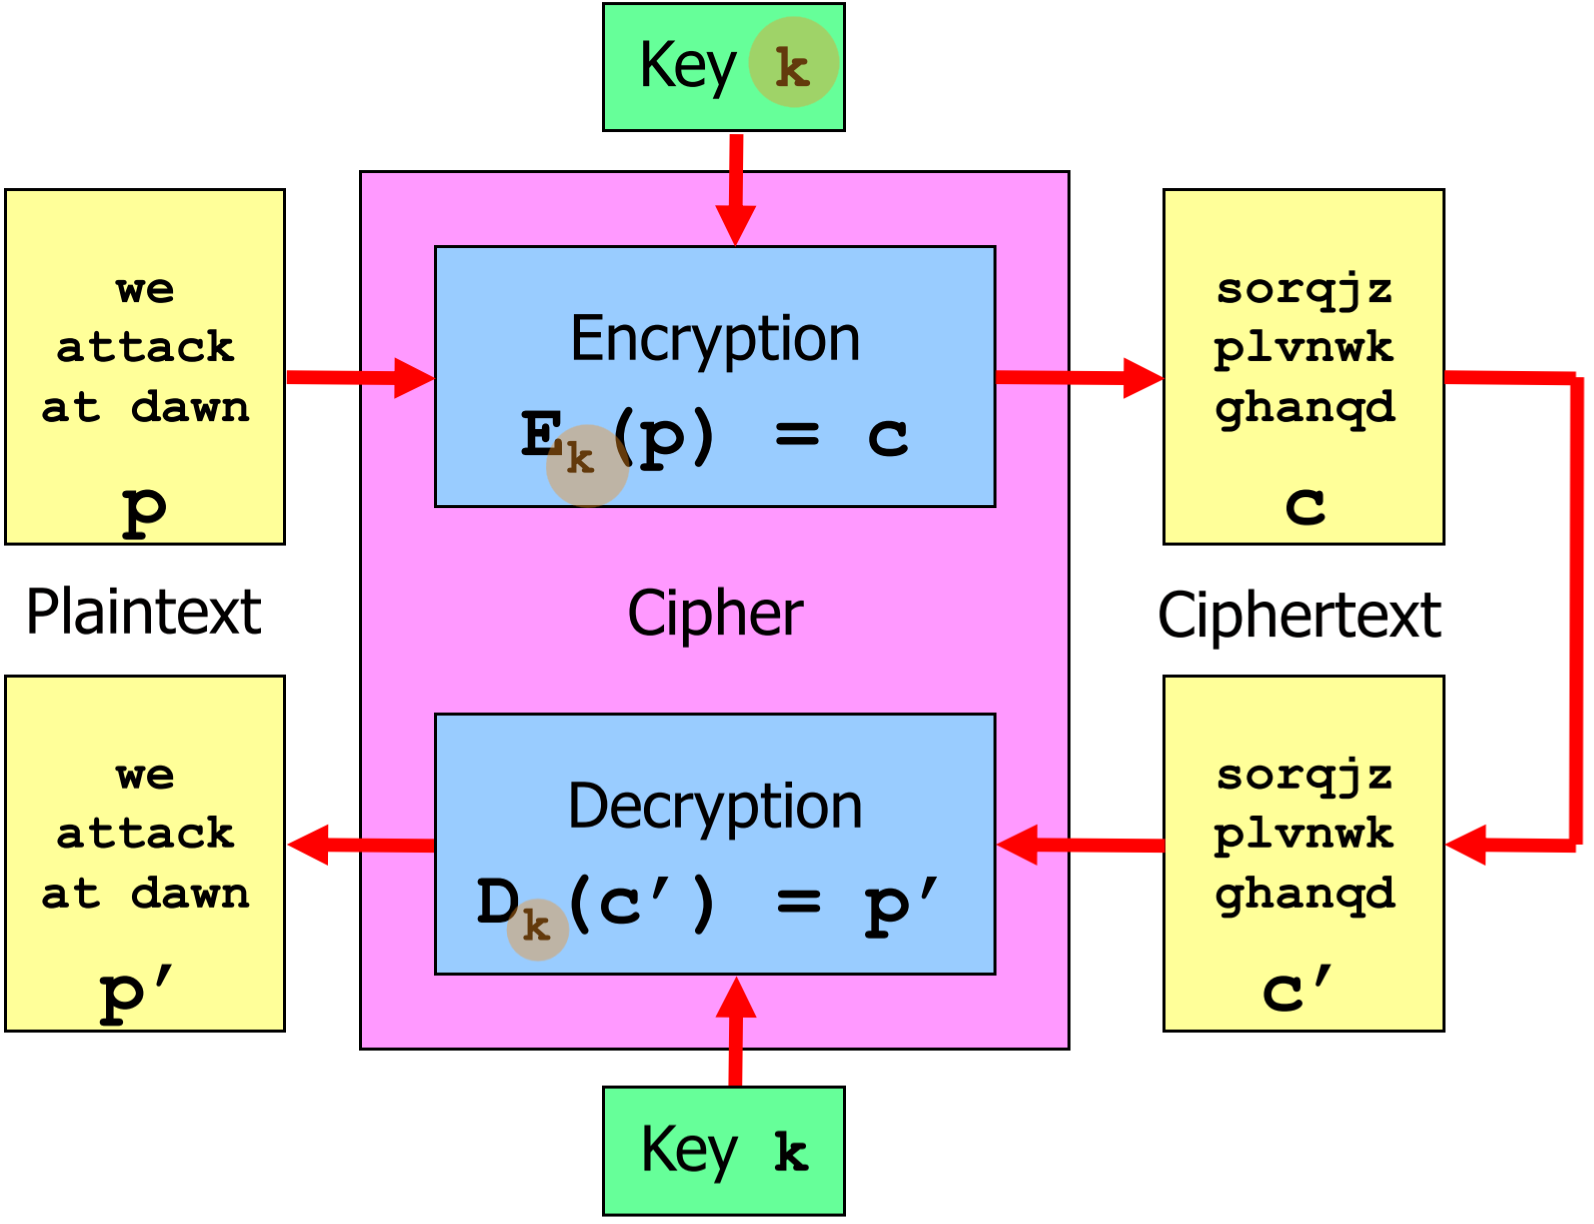
\includegraphics[width=150px]{img/BasicTerminologySecKeyCrypto.png}
	\captionof{figure}{Basic Terminology basierend auf Secret Key Cryptography}
	\label{fig:Basic Terminology}
\end{Figure}
\begin{itemize}
	\item Die Verschlüsselung ist eine Transformation von $P$ (Set von Plaintexte) zu $C$ (Set von Ciphertexts) unter der Anwendung von $K$ (Set von Keys)
	\item Grundidee ist, dass man nicht einen einzigen Key hat, jedoch eine Vielzahl von Transformationen, wobei jeder Key einen andere Transformation nachvollzieht
	\item $c = E(k,p)$ oder $E_K(P)$
	\item $p = D(k,c)$ oder $D_K(c)$
	\item Jede Transformation (jede Wahl des Schlüssels) muss reversibel (injektiv) sein. $\Rightarrow$ $|C|$ kann nicht kleiner sein wie $|P|$, meistens gilt $P = C$
\end{itemize}

	
	\subsection{Kryptoanalyse}
Hingegen befassen sich Kryptoanalysten mit der Kryptoanalyse, welches die Kunst und die Wissenschaft rund um das Entschlüsseln von \textit{Ciphertext} ist.

\section{Sie können Shannons grundlegende Konzepte definieren: Information, Entropie, vollkommene Geheimhaltung und sein Modell eines Kryptosystems mit geheimen Schlüssel}
Claude Shannon: \textit{"Um das Problem mathematisch lenkbar zu machen, gehen wir davon aus, dass der Feind das verwendete System kennt. Das heißt, er kennt die Familie der Transformationen [E(k, p) und D(k, c)] und die Wahrscheinlichkeiten der Wahl verschiedener Schlüssel.}
\begin{Figure}
\centering
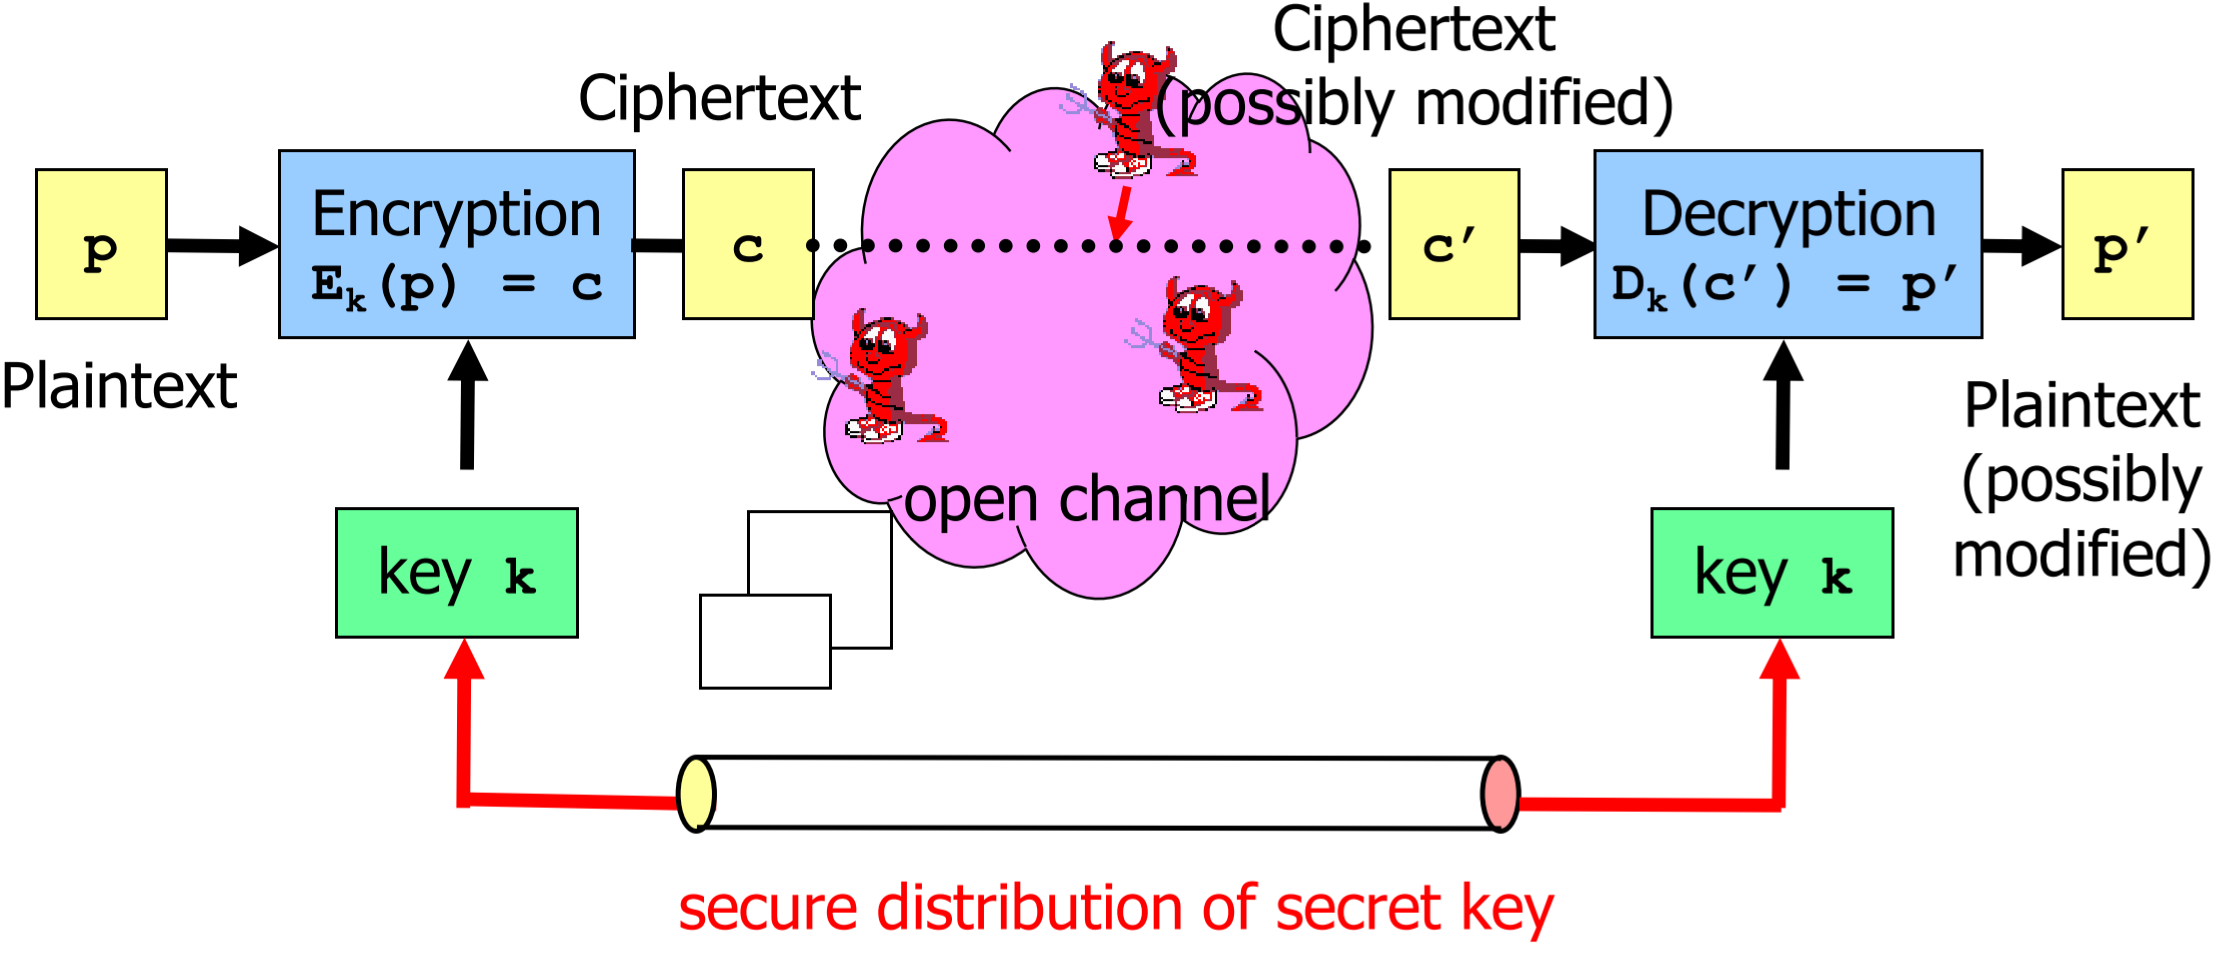
\includegraphics[width=150px]{img/ShannonsModel.png}
	\captionof{figure}{Shannon's Model von einem Secret Key Cryptosystem}
	\label{fig:Basic Terminology}
\end{Figure}
\begin{itemize}
	\item Der gleiche Key / Schlüssel wird für das Verschlüsseln und Entschlüsseln verwendet
	\item Der Key muss absolut geheim sein
	\item \textbf{Schlüssel-Verteil-Problem} $\rightarrow$ Der Schlüssel muss über einen vertraulichen und authentifzierten Kannel erfolgen
\end{itemize}
Problem dabei ist, dass der Kanal nicht sicher ist, Encyrpt und Decrypt hat denselben Key und die Verteilung des Schlüssel muss sicher erfolgen.

	\subsection{Entropy - Informationsgehalt messen}
Wenn die Schlüssel nicht mit der gleichen Wahrscheinlichkeit gewählt wurden, und der Angreifer das weiss, dann macht das das Leben des Angreifers um einiges einfacher.

		\subsubsection{Definition}
Nehmen wir eine zufällig endlich gewählte Variable $X$ mit $n$ Ergebnisse, wobei $p(i) = P(X=i)$ die Wahrscheinlichkeit des Ergebnisses $i$ ist. Wenn die Wahrscheinlichkeit $P(i)$ gross bzw. klein ist, ist das Ergebnis (nicht) überraschend. $\Rightarrow$ $\log_2 \frac{1}{p(i)}$ definiert aus diesem Grund den Überraschungsfaktor.\\
\textbf{Formel} Die Entropy(H) von X, wird in Bits gemessen und ist die durchschnittliche Überraschung des Ergebnis\\
\begin{equation}
	H = \sum_{i=1}^n p(i) \log_2(\frac{1}{p(i)}
\end{equation}
\textbf{Maximale Entropy}: wird erreicht wenn alle Ergebnisse gleich wahrscheinlich sind. $\rightarrow$ In diesem Fall ist es am schwierigsten das Ergebnis im Vorfeld zu erraten\\
\textbf{unabhängige Ereignisse}: Wenn die Experimente unabhängig sind, dann ist die Entropy additive. $\rightarrow$ Durch $\log_2$ liefert $n+1$ bits immer zweimal so viel Informationen wie $n$ Bits. Wobei 4 Bits nicht zweimal so viel Information wie 2 Bits liefern, jedoch $\frac{2^4}{2^2} = \frac{16}{4} = 4$ so viel Information

		\subsubsection{Fairer Münzwurf}
Die Entropy eines fairen Münzwurfs ($\rightarrow$ $p_{heads} = p_{tails} = 0.5$) wird wie folgt berechnet
\begin{equation}
	H = 0.5 * \log_2(2) + 0.5 * \log_2(2) = 2 * 0.5 *\log_2(2) = 1 Bit
\end{equation}
$\Rightarrow$ Ein fairer Münzwurf liefert 1 bit Information

		\subsubsection{Unfairer Münzwurf}
Die Entropy eines unfairen Münzwurfs ($\rightarrow$ $p_{heads} = 0.25 p_{tails} = 0.75$) wird wie folgt berechnet
\begin{equation}
	H = 0.25 * \log_2(4) + 0.75 * \log_2(2) = 2 * 0.5 *\log_2(\frac{4}{3}) \approx 0.81 Bit
\end{equation}
$\Rightarrow$ Ein unfairer Münzwurf liefert 0.81 bit Information $\rightarrow$ liefert weniger Information als ein fairer Münzwurf, da beim unfairen Wurf das Ergebnis einfacher zu erraten ist. Wäre es ein komplett unfairer Wurf und es kommt immer Kopf, so würde es 0 Bit Information liefern.

		\subsubsection{Entropy für Passwörter}
Die Auswahl eines Passworts kann ebenfalls als ein Resultat eines zufälligen Experiments betrachtet werden.\\
\\
\begin{itemize}
	\item \textit{Ein Passwort beinhaltet 8 zufällige Hexadezimal Zeichen (0-9, A-F)} $\rightarrow$ $2^4$ Möglichkeiten pro Zeichen $\rightarrow$ $(2^4)^8 = 2^{32}$ gesamtmögliche Anzahl Passwörter
	\item \textit{Der konstante String '0000 0000'} $\rightarrow$ nur ein Passwort: $H = \log_2(1) = 0 bits entropy$, wobei es nicht nur 00000 ist, sondern dass es einen konstanter String ist. Sprich bspw. nur ABCD oder 010101 wäre ebenfalls mit 0 Bit Entropy betitelt.
\end{itemize}

	\subsection{Security of cryptosystems}
\begin{itemize}
	\item Muss resistent gegen die Angriffe sein 
	\item Braucht einen genügend grossen Workfactor
	\item Should reveal as little as possible about the plaintext
	\item By construction, a plainttext letter could never be enciphered to itself
\end{itemize}

	\subsection{vollkommene Geheimhaltung}
\begin{itemize}
	\item Ein System auf welches die Eigenschaften eines sicheres Cryptosystem zutrifft, wird \textbf{Information-theoretically secure} genannt (oder nach Shannon (\textit{has perfect secrecy})
	\item Es gibt genau ein Sytem, welcher diese Anforderungen erfüllt und das ist ein One-Time-Pad
\end{itemize}
		
\section{Sie können einen kryptografischen Arbeitsfaktor definieren und verstehen, warum $2^128$ (manchmal $2^256$) ein guter Arbeitsfaktor (work factor) ist}
$\rightarrow$ work factor $=$ average number of keys to try
	\subsection{Work Factor / Arbeitsfaktor}
\begin{itemize}
	\item Manchmal ist bei einem gegeben C, nur ein K sinnvoll, so dass $p = D(k,c)$ gilt und alle andere Keys keinen Sinn ergeben $\Rightarrow$ in einem solchen Fall kann man den Schlüssel durch einfaches Ausprobieren (Brute-Force) und sehen, wann der Plaintext Sinn ergibt. $\rightarrow$ Dafür muss man die Länge des Keys in etwas abschätzen können
	\item Die durchschnittliche Dauer / Anzahl welche es benötigt, bis der richtige Key gefunden wird, wird als \textbf{work factor / Arbeitsfaktor} betitelt 
	\item Wenn wir von einer dreistelligen Zahl (0,..,9) ausgehen gibt es $10^3 = 1'000$ Kombinationsmöglichkeiten $\rightarrow$ unter der Annahme, dass alle Zahlen gleich wahrscheinlich sind, beträgt der work factor $= 500.5$ $\Rightarrow$ bei 4 Zahlen ($10^4 = 10'000$) beträgt der work factor $=5000.5$
	\item Wenn man eine Zahl hinzufügt, steigt der Aufwand exponential $\rightarrow$ Mein Aufwand steigt um eins, der von der Drittperson um den Faktor 10
	\item Falls es keine Shortcuts gibt, ist die Vergrössung des secrets eine gute Idee
	\item Wenn alle Keys gleichwahrscheinlich sind, ist der work factor $\approx$ $0.5*$key space size
	\item Der work factor ist normalerweise gegeben in bits: $\log_2$(\textit{key space size})
\end{itemize}

	\subsection{Was bedeutet gross genug?}
Annahme: \textit{Angreifer kann 1 key  in 1ps ($10^{-12}$) auf einem Computer ausprobieren. Wobei der Angreifer 1 Milliarde Computers hat}\\
\textbf{32 Bits genügend?} $\rightarrow$ $2^{32} = 4*10^9$ entsprechend braucht der Angreifer $0.5*4*10^9$keys$10^{-12}$s/(keys/computer)/1 computer $=2$ms mit einem Computer\\
\textbf{64 Bits genügend?} $\rightarrow$ $2^{64} = 1.8*10^{19}$ entsprechend braucht der Angreifer $0.5*1.8*10^{19}$keys$10^{-12}$s/(keys/computer)/$10^{19}$ computer $=0.01$s mit allen Computer\\
\textbf{128 Bits:} $\rightarrow$ braucht $0.5*10^{17.5}$s $=5*10^9$ Jahren $\Rightarrow$ gross genug\\
\textbf{256 Bits:} $\rightarrow$ braucht $0.5*10^{56}$s $=10^{48}$ Jahren $\Rightarrow$ gross genug

	\subsection{Beziehung zwischen Entropy und work factor}
\textbf{Ergänzen mit zusätzlichen Slides vom OLAT}
Der Workfactor muss nicht 0.5-Entropie sein! $\rightarrow$ Die Aussage, dass der Workfactor der Hälfte der Entropy ist, stimmt nicht in jedem Fall, dies ist abhängig von der Strategie wie man Brute-Force durchführen wird.

\section{Sie können ein One-Time-Pad definieren und seine Eigenschaften benennen}
\begin{itemize}
	\item Ist ein \textbf{Informatino-theoretically secure}
	\item Auch Vernam Cipher genannt
	\item jedes Bit hat die gleiche Wsk
	\item jedes Bit ist unabhängig vom anderen
	\item Schlüssel ist gleich lang wie der Plaintext
	\item Verschlüssung ist eindeutig $\Rightarrow$ Die Menge aller Klartexte (P) und die Menge aller Verschlüsselungen (C) sind injektiv. Dies bedeutet, dass jedes Element in P genau ein Element in C hat
	\item Des Weiteren gilt die Surjektivität, sprich jedes Element in C hat genau eine Abbildung in P.
	\item Daraus folgt $|P| = |C|$
	\item wir brauchen so viele Schlüssel wie wir Text haben
	\item Dies erfolgt durch eine XOR-Verknüpfung
	\item \textbf{WICHTIG} Für jeden Plaintext wird ein neuer Key verwendet. Dies gilt für alle jemals erstellten und alle welche in Zukunft erstellt werden. $\rightarrow$ Andernfalls würde die Bedingung der eindeutigen Abbildung nicht mehr gelten. Ein Key darf nicht wiederverwendet werden.
	\item Der Schlüssel ist im Vorfeld bekannt und beide Seiten kennen diesen Schlüssel.
\end{itemize}

\begin{Figure}
\centering
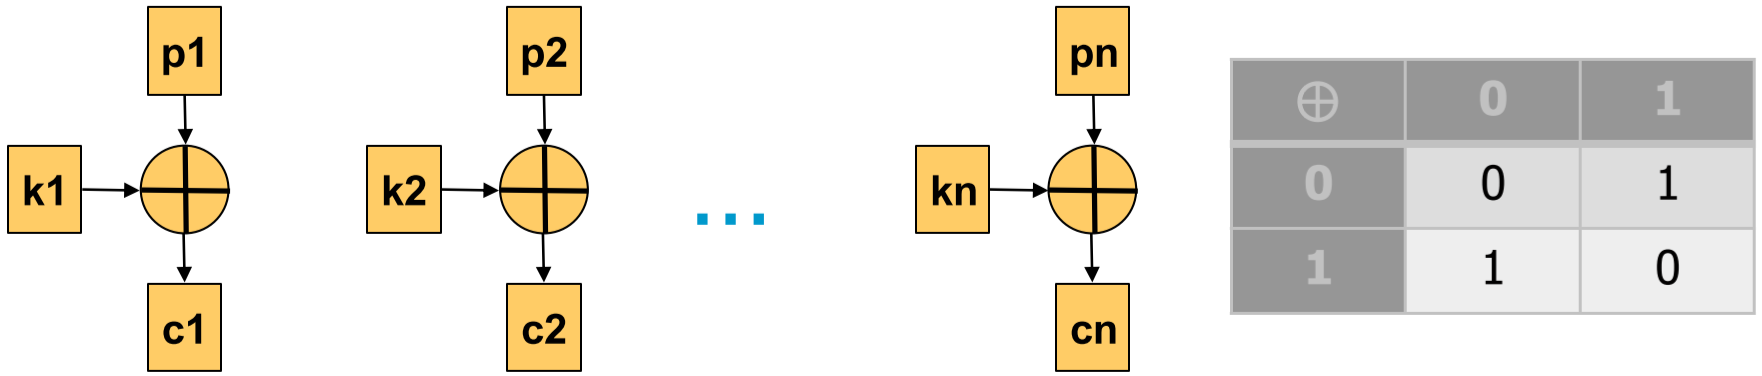
\includegraphics[width=150px]{img/OneTimePad.png}
	\captionof{figure}{One Time Pad}
	\label{fig:One Time Pad}
\end{Figure}

Da One-Time Pad nicht immer praktikabel ist, werden die Eigenschaften etwas abgeschwächt. 
\begin{itemize}
	\item Gleicher Key für encrypt und decrypt
	\item Falsche Keys geben eine hohe Entropy als Ergebnis $\rightarrow$ can usually tell when correct key used
	\item guter moderner cipher $\rightarrow$ key entropy $\approx$ work factor
	\item Design-Parameter block-size und key-size
	\item Heute AES (Advanced Encryption Standard) standard
\end{itemize}

Nach Information-theoretically Secure, folgt \textit{computational security (work factor $\approx$ key entropy}. Problematik dabei ist, dass es keinen Beweis gibt, dass der Algorithmus computationally secure sicher ist.\\
\textit{Hinweis:} Hashing-Verschlüsselungen sind am Altern, unteranderem weil man immer mehr Computer-Power hat

\section{Sie können das Zufallsorakel-Modell der Secret-Key Ciphers definieren und seine Konsequenzen benennen}
\textbf{Prüfungsrelevant}\\
Das Random-Oracle Model ist ein allgemeines Model

\textbf{Vorbedingungen:}
\begin{itemize}
	\item P entspricht einem Set von allen Plaintexten
	\item C entspricht einem Set aller Ciphertexts
	\item K entspricht einem Set von allen Keys
	\item Wir nehmen an, dass $P=C$
\end{itemize}

\textbf{Eigenschaften:}
\begin{itemize}
	\item TBD
\end{itemize}

\textbf{Vorgehen:}
\begin{itemize}
	\item TBD
\end{itemize}

\chapter{Vorlesung 2 - Secret Key Cryptography}

\section{Sie verstehen das Konzept der Block- und Stream-Cipher und wissen, wie sie in der Praxis eingesetzt werden}
Wenn wir das Prinzip des Secret Key Cryptography von Shannon hervornehmen, erinnern wir uns, dass derselbe Schlüssel für die encryption, sowie für die decryption verwendet wird (dieser muss absolut geheim sein). Der gleiche Key kann für mehrere Nachrichten verwendet werden, dieser Key sollte jedoch periodisch ausgewechslet werde $\rightarrow$ Verteilungsproblem
	
	\subsection{Block-Ciphers}
\begin{Figure}
\centering
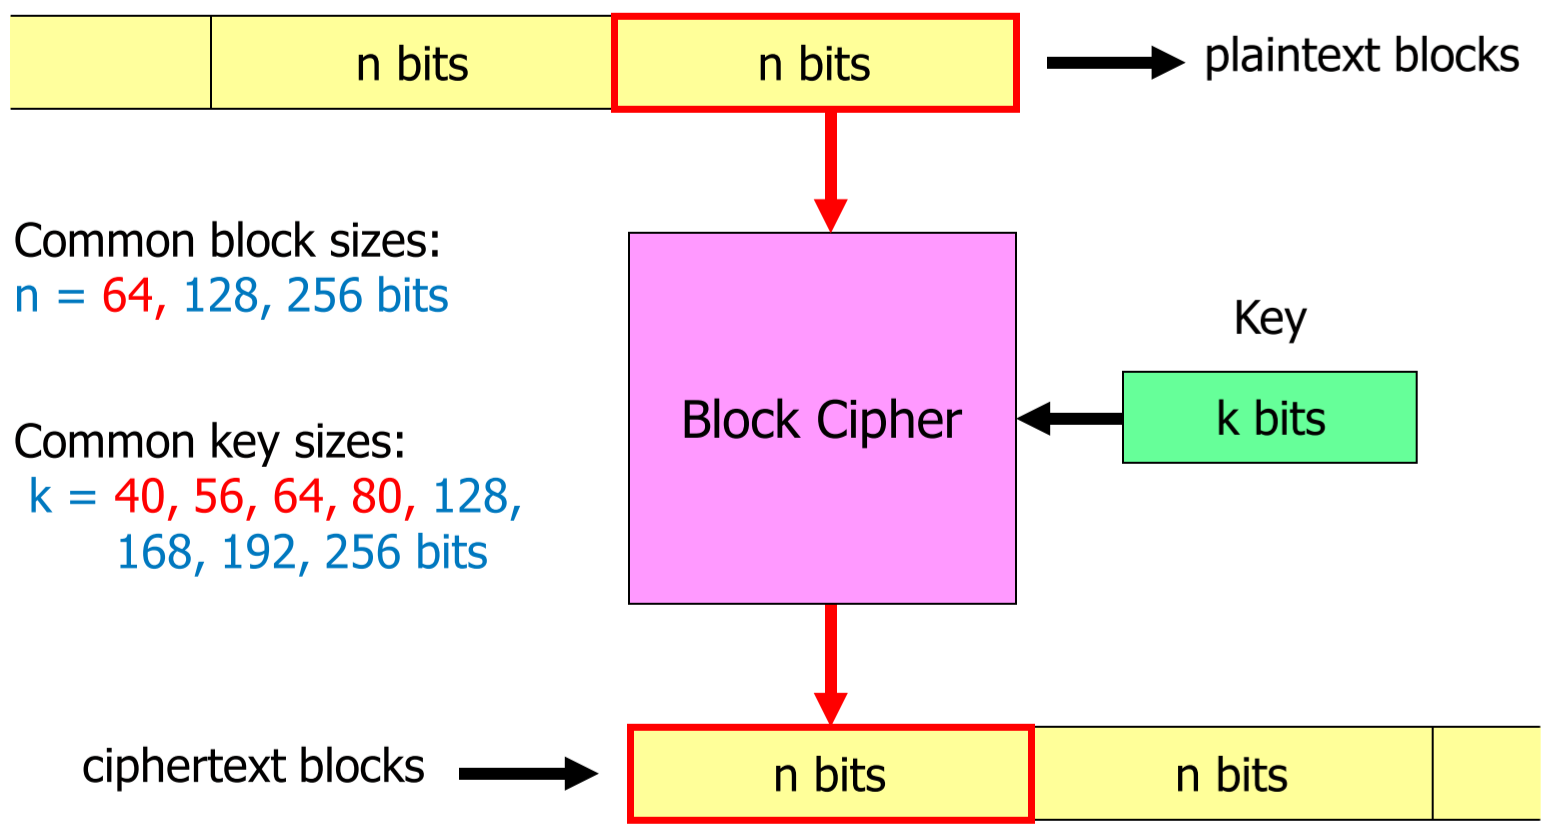
\includegraphics[width=150px]{img/BlockCiphers.png}
	\captionof{figure}{Block Ciphers}
	\label{fig:Block Ciphers}
\end{Figure}

\begin{itemize}
	\item Block-Ciphers schneidet einen Klartext beliebiger Länge in eine Reihe von Blöcken mit konstanten Grösse von n Bit auf
	\item Anschliessend wird jeweils einen Klartextblock verschlüsselt und entsprechend als Block-Cipher dargestellt.
	\item Jeder Schlüssel muss von einem Klartextblock zu einem Ciphertextblock führen (1:1 Abbildung), andernfalls könnte ein Ciphertextblock nicht eindeutig entschlüsselt werden.
	\item Die Feistel-Chipher ist eine gängige Art von Block Ciphers, welche diese Eigenschaften per Design erfüllen.
\end{itemize}

		\subsubsection{Common Block Sizes}
\begin{itemize}
	\item Bis Mitte 90er Jahre war 64Bit die gebräuchliche Länge
	\item Ab 2011 128 als Mindestschlüssellänge angenommen um Brute-Force-Angriffe zu verhindern
	\item 8, 16, 32 Bit Blockgrössen sind nicht sicher $\rightarrow$ ANgreifer lernt die Paare indem er bspw. eine Tabelle führt $\Rightarrow$ bei 16 Bit sind dies bspw. nur $2^{16}$ Paar-Möglichkeiten
	\item Bei 64-Bit-Blöcken hätte diese Tabelle bereits $2^{64}$ Einträge (=16 exa-Einträge). Es ist sehr unwahrscheinlich, dass ein Angreifer so viele Klartext-Chiphertext-Paare, die den gleichen Schlüssel verwenden, sowohl akkumulieren als auch speichern kann
\end{itemize}

		\subsubsection{Common Key Sizes}
Schlüsselgrössen mit 40, 56 und 64 Bit sind eindeutig unsicher und sollten nicht mehr verwendet werden. Verwenden Sie sicherheitshalber eine Schlüsselgrösse von 128 Bit oder mehr.

		\subsubsection{Randomness of the mapping}
\begin{itemize}
	\item Ein guter Block-Cipher hat die Eigenschaft, dass die Zuordnung von Plaintext-Block zu einem generierten Ciphertext-Block bei einem beliebigen Schlüssel zufällig aussieht $\rightarrow$ als ob die Bits des Ciphertext-Block durch das Werfen einer fairen Münze erzeugt wurde
	\item Wenn die Abbildung eine gute Zufallseigenschaft hat, ist es für den Angreifer sehr schwierig, Informationen über einen Plaintext-Block durch Betrachtung des entsprechenden Geheimtextblocks abzuleiten
	\item Aus mathematischer-Sicht sind dann der Plaintext-Block und der Ciphertext-Block \textit{so unabhängig wie möglich} $\rightarrow$ Änderungen eines einzelnen Bits in einem Plaintext-Block führen zu einem völlig anderen Ciphertext-Block $\Rightarrow$ Dies erreicht man in dem jedes der n Bits des Chiffrierblocks eine Funktion aller n Bits des Klartextblocks und der k Bits des geheimen Schlüssels sein. DES erreicht dies beispielsweise durch geschickte Verwechslungs- und Diffusionsoperationen 
\end{itemize}

\section{Sie kennen die wichtigsten Block- und Stream-Cipher und können anhand der Schlüssellänge eine Aussage über deren kryptographische Stärke machen}

	\subsection{Data Encryption Standard (DES)}
	
	\subsection{Triple DES}
	
		\subsubsection{Meet in the Middle Attack (Known-Plaintext Attack}
\begin{itemize}
	\item Triple DES wird in zwei Teilen unterteilt
	\item Sämtliche $2^112$ Varianten werden in einer Tabelle dargestellt
	\item Ebenso wird eine Tabelle für $2^56$ erstellt
	\item Danach werden in den beiden Tabellen nach Paaren gesucht, bei Übereinstimmung hat man den Key
\end{itemize}

\begin{Figure}
\centering
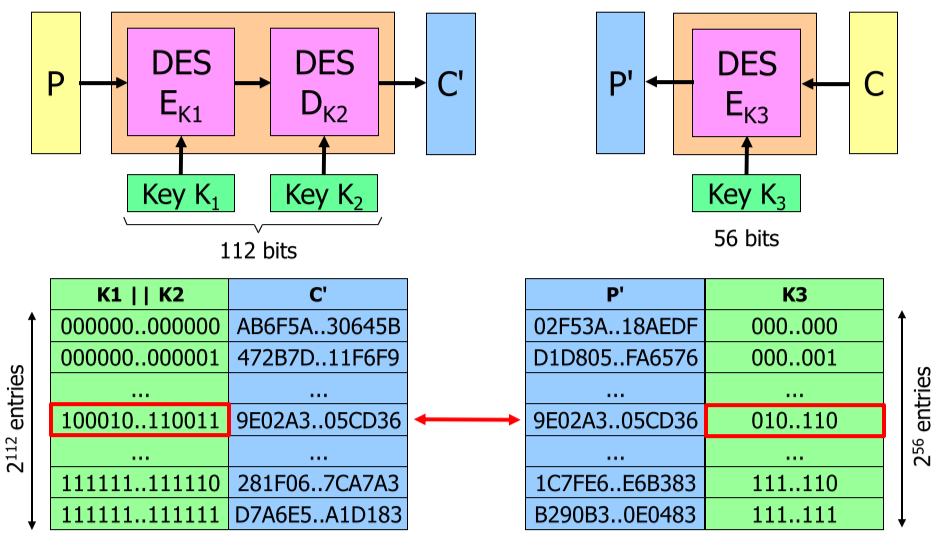
\includegraphics[width=150px]{img/MeetInTheMiddleAttack.png}
	\captionof{figure}{Meet in the Middle Attack}
	\label{fig:Meet in the Middle Attack}
\end{Figure}

	\subsection{Advanced Encryption Standard (AES)}
\begin{itemize}
	\item Stand jetzt ist die beste Möglichkeit einen AES zu knacken, ist mit dem Brute-Force Vorgehen
\end{itemize}

\textbf{Requirements}\\
\begin{itemize}
	\item Sollte ein symmetrischer Block Cipher sein
\end{itemize}



\section{Sie verstehen die verschiedenen Blockchiffriermodi, ihre Stärken und Schwächen und kennen ihre Anwendungen}

	\section{Block Cipher Mode}
\textbf{Electronics Code Book Mode (ECB)}\\
$\Rightarrow$ 
\begin{Figure}
\centering
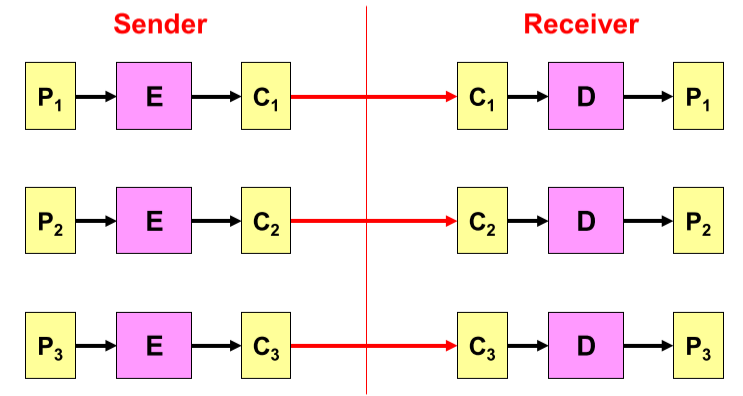
\includegraphics[width=150px]{img/ECB.png}
	\captionof{figure}{Electronic Code Book Mode}
	\label{fig:Meet in the Middle Attack}
\end{Figure}

		\subsubsection{Cipher Block Chaining Mode (CBC)}
\begin{itemize}
	\item XOR-Verknüpfung mit dem vorherigen CipherBlock
	\item Das Inverse der XOR-Verknüpfung ist wiederum die XOR-Verknüpfung	
	\item es entsteht eine Abhängigkeit 
	
\end{itemize}

	\section{Stream Cipher}


\chapter{Vorlesung 4 - Data Integrity and Authentication}

\section{Sie kennen das prinzipielle Konzept einer Einweg Hash-Funktion}
\begin{itemize}
	\item Die Hash-Funktion mappt eine variable-Länge von bit strings als Input (Nachricht) zu einer fixen Grösse als Output-String (Der Hash oder message digest) $\rightarrow$ many-to-one-mapping
	\item Typische Hash-Länge sind: 128, 160, 256, 512
	\item Alle Eigenschaften erfüllt: In der Praxis erzeugt eine Nachricht einen eindeutigen Hash, und ein Hash gehört zu einer bestimmten Nachricht $\rightarrow$ Verwendung des Hash als Stellvertreter für die Nachricht selbst
\end{itemize}

\textbf{Wichtige Eigenschaften}\\
\begin{itemize}
	\item Der Hash kann effizient berechnet werden, auch wenn die Länge der Nachricht mehrere Gigabytes gross ist $\rightarrow$ Da das Dokument in der Regel viel grösser als der Hash-Wert ist, ist die Abbildung eine many-to-one Funktion. Für jeden spezifischen Hash-Wert gibt es potenziell viele Dokumente, die diesen Fingerabdruck besitzen. 
	\item Das Mapping sollte pseudo-zufällig passieren $\rightarrow$ Es gibt keine Verbindung zwischen der Nachricht und ihrem Hash. Der Hashwert der Nachricht sollte von jedem Bit entsprechenden Nachricht abhängen. Wenn ein einzelnes Bit der Originalnachricht seinen Wert änder oder ein Bit hinzugefügt oder gelöscht wird, dann sollten etwa 50 Prozent der Digest-Bits ihre Werte in zufälliger Weise ändern.
	\item Wenn man einen Hash gegeben hat, ist es praktisch unmöglich die Nachricht zu finden, welchen diesen Hash produziert (\textbf{preimage resistance})
	\item Es ist praktisch unmöglich zwei Nachrichten zu finden, welchen zum gleichen Hash-Wert mappen (\textbf{collision resistance}
\end{itemize}

	\subsection{Hashes / Message Digests}
Ein Hash mit einer fixen Grössen agiert als eindeutiger Fingerabdruck für eine Nachricht (Dokument etc.) mit willkürlicher Grösse. Mit einer gewöhnlichen Verwertungsgrösse (digests-size) von 128 .. 256, gibt es $10^{38}$ .. $10^{77}$ verschiedene Fingerabdruckmöglichkeiten. 

	\subsection{Populäre Hash-Funktionen}
\begin{itemize}
	\item MD5 $\rightarrow$ Message Digest Number 5 $\Rightarrow$ geknackt
	\item SHA 1 $\rightarrow$ Secure Hash Algorithm Number 1 $\Rightarrow$ geknackt
	\item SHA 2 $\rightarrow$ Secure Hash Alogrithm Number 2 $\Rightarrow$ wird als sicher angesehen
\end{itemize}

	\subsection{Merkle-Damgard Construction of hash Functions}
\textit{Vorlesung 4 - Slide 9 evtl ergänzen}
\textit{Vorlesung 4 - Slide 13 evtl ergänzen}


\section{Sie wissen wie man Integrität und Authentizität einer Nachricht / Dokument mittels message authentication codes und digitalen Signaturen schützt}


	\subsection{Message Authentication Codes}	
Ein digitaler "message digest" selbst bietet noch keinen Schutz gegenüber unauthorisierter Änderungen eines Dokuments oder Nachricht. Nach jeder Änderung an einem Dokument gibt es einen neuen gültigen Hashwert welcher auf den neuen Inhalt berechnet wird. \\
Einzig mit der Einführung eines \textit{secret keys} in Form eines berechneten Fingerabdrucks kann ein Dokument gegen unbefugte Veränderungen gesichert werden. Nur der Eigentümer dieses Keys kann die Nachricht entsprechend auswerten $\rightarrow$ \textbf{Message Authetnication Code (MAC)}. Dabei muss natürlich der Empfänger des sicheren Dokuments im Besitz des secret Keys sein. Dies um die Nachricht entsprechend zu verifizieren und validieren, dies wird mittels Berechnung und Vergleich des \textbf{Message Authentication Codes (MAC)-Werts}. $\Rightarrow$ Manchmal wird MAC auch als \textbf{Message Integrity Check (MIC)}

	\subsection{Digital Signatures}
Die ursprüngliche Idee von digitalen Siganturen war, dass man etwas identisches zur handgeschriebenen Signatur zur Unterzeichnung von digitalen. Entsprechend sollten auch deren Eigenschaften sein:\\

\begin{itemize}
	\item Die Signatur sollte nicht einfach zu fälschen sein
	\item Jeder kann die Gültigkeit der Signatur validieren
	\item Die Signatur ist zu einem Dokument gebunden
	\item Die Unterschrift kann nicht zurückgewiesen werden, $\rightarrow$ der Unterzeichner kann sich später nicht darauf berufen, dass er das Dokument nicht unterschrieben hat.
\end{itemize}	
Eine Möglichkeit dies umzusetzen ist mit \textit{public key cryptography}

		\subsubsection{digitale Signaturen mittels public Key Cryptography}
Um eine Dokument oder Nachricht zu \textit{unterschreiben}, wird ein \textbf{private key} verwendet $\rightarrow$ Nur der Eigentümer des private key kann die Signatur erstellen\\
Um eine Signatur zur \textit{verifizieren}, wird ein \textbf{public key} verwendet $\rightarrow$ jeder kann die Signatur verifizieren\\
\textbf{Notation}
\begin{equation}
\begin{split}
	Signatur \Rightarrow S_{K_Priv} (M) &= Sig_M\\
	Verify \Rightarrow V_{K_Pub} (M, Sig_M) &= true / false
\end{split}
\end{equation}

	\subsubsection{Vorgehen}
\begin{Figure}
\centering
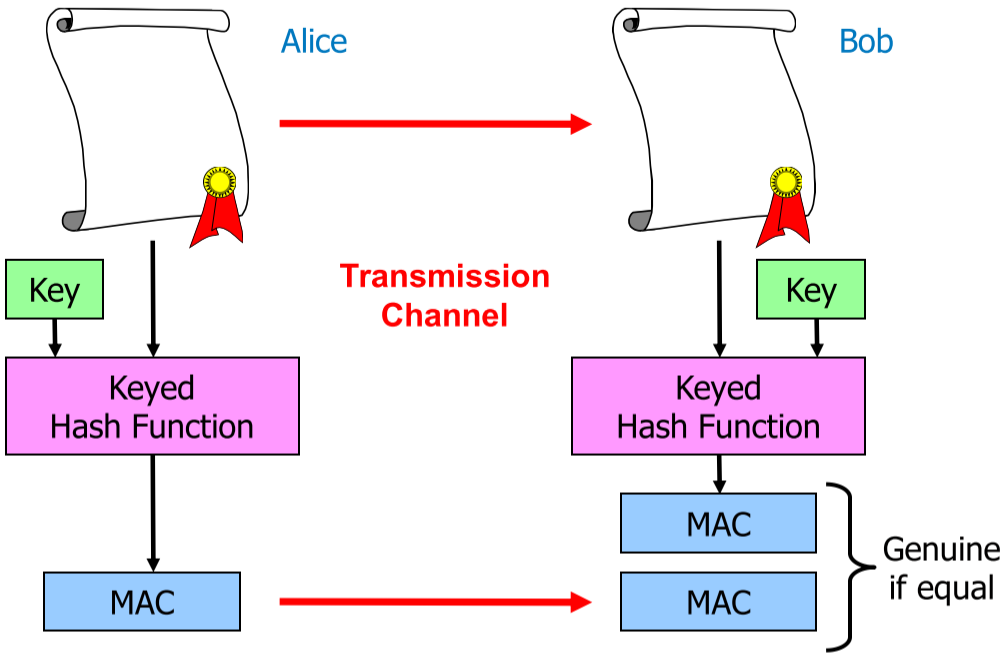
\includegraphics[width=150px]{img/MessageAuthenticationCodes.png}
	\captionof{figure}{Message Integrity / Authenticity with Message Authentication Codes}
	\label{fig:Message Integrity / Authenticity}
\end{Figure}
\begin{enumerate}
	\item Alice berechnet mittels der Hash-Funktion den Hash-value zusammen mit dem Private-Key entsteht die Signatur
	\item Bob kann die Berechnung nicht von oben nach unten durchführen, denn ihm fehlt die Information des private Keys. 
	\item Jedoch kann Bob den Hash berechnen
	\item Bob kann die Signatur mittels dem Public Keys zurück berechnen und erhält einen neuen Hash-Wert
	\item Bob vergleicht nun die beiden Hash-values
\end{enumerate}
	
\section{Sie verstehen wie schwierig es ist eine Nachricht zu fälschen oder zu kollisionen}
	\subsection{Fälschung}
Ziel ist es durch einen zufälligen Text und der Hash-Function den gleichen Hash-value zu haben. Denn der Hash-value ist repräsentativ für das Dokument. Gelingt einem dies, so können wir dies entsprechend fälschen ohne, dass es bemerkt wird.\\
Wenn der Hash-value m bits lang ist, braucht man im Durchschnitt $2^{m-1}$ (halb so viele) Versuche um das Dokument zu verfälschen.\\

$\Rightarrow$ Das Birthday-Paradox-Beispiel ist das gleiche Problem, wie ein Dokument zu finden mit dem identischen Hash

	\subsection{Kollision}
Eine Kollision ist, dass irgendwelche zwei Dokumente denselben Hash-Wert haben. Dies ist im Vergleich zur Fälschung um einiges einfacher, als bei einem gegegeben Dokument mit einem gegegebenen Hash-value, einen identischen Hash-Value zu finden
		\subsubsection{Birthday Attacks}
Birthday Attacken kann man auch gegen Hash-Funktionen anwenden. Man fügt dem original Dokument und dem gefälschten Dokument neuen zufälligen Text hinzu und überprüft ob die Hash-Werte identisch sind.
$\Rightarrow$ Alleine aus diesem Grund sind MD5 und SHA-1 nicht mehr sicher. Aus diesem Grund muss die Kryptographie Kollision resistent sein

	\subsection{MD5-Security}
\begin{itemize}
	\item ist nicht kollissionsfrei 
	\item Ab 2007 war es sehr einfach solche Dokumente mit dieser Hash-Funktion zu kollidieren
	\item nicht trivial, braucht man $\approx 2^{50}$ MD5-Berechnungen
	\item Selbst wenn MD5 eine vernünftige Länge hätte, sollte MD5 nicht verwendet werden
\end{itemize}

	\subsection{SHA-1 Security}
\begin{itemize}
	\item Nicht viel besser
	\item Work-factor inkl. möglichen Abkürzungen braucht man $2^{63}$ Berechnungen für eine Kollissino
	\item Ist kompromentiert $\Rightarrow$ nicht mehr verwenden
\end{itemize}

	\subsection{SHA-2 und SHA-3}
\begin{itemize}
	\item Für SHA-2 gibt es keine bessere Möglichkeit als mit Brute-Force anzugehen
	\item die NSA war bei der Erstellung dieser Hash-Funktion mitbeteiligt
	\item Trotzdem kann man diese ohne Sorgen verwenden
	\item noch nicht klar ob SHA-3 die dominante Hash-Funktion sein wird. $\rightarrow$ grundsätzlich sollte man momentan auf SHA-2 bleiben, jedoch SHA-3 im Hinterkopf behalten
\end{itemize}

\section{Sie wissen wie Verschlüsselung und Integritäts-Schutz kombiniert werden sollen, um sich vor Angriffen zu schützen}
Wir haben festgestellt, dass reine Verschlüsselung uns nicht den vollständigen Schutz bietet, da man durch andere Attacken trotzdem das Dokument nicht vollständig schützen kann. Aus diesem Grund sollte man immer sowohl eine Verschlüsselung anwenden, wie auch einen Integritätsschutz. Dafür hat man zwei Möglichkeiten:
\begin{enumerate}
	\item Berechnung des MAC mittels Plaintext und hängt den MAC an den Plainttext und verschlüsselt den Plaintext und MAC $\rightarrow$ \textit{MAC then encrypt}
	\item Verschlüsselung Plainttext, Berechnung eines MAC mittels Ciphertext und hängt diesen an den Ciphertext an $\rightarrow$ \textit{Encyrpt then MAC}
\end{enumerate}

In der Theorie sind beide Möglichkeiten gleich sicher. Dies sieht jedoch in der Praxis anders aus, in der Praxis funktiontiert \textit{Encrypt then MAC} besser. 

	\subsection{Handlungsempfehlung}
\begin{enumerate}
	\item Niemals nur Verschlüsselung, sondern immer noch Integritätsschutz miteinbauen
	\item Falls das nicht geht, sollte man im Minimum MAC, zusammen mit encyrpt-then-MAC verwenden
	\item Bei der Entschlüsselung, sollte man bei einer Fehlermeldung immer alles bereits entschlüsselte Wegwerfen und nicht an den Benutzer aushändigen
\end{enumerate}

	\subsection{Galois/Counter Mode}
	\textbf{Vorteile}
	\begin{itemize}
		\item Performanter
		\item offizieler NIST-Standard
		\item Es ist eine integrierte Lösung von Verschlüsselung und Integritätsschutz
		\item Es folgt dem encrypt-then-MAC-Prinzip
	\end{itemize}

\section{Sie wissen wie Passwörter für die Authentifizierung verwendet wird und kennen die best-practice Ansätze vor dem Gebrauch von Passwörtern}
Passwörter sind grundsätzlich sehr populär und einfach zu implementieren.\\

Prinzipien:\\
\begin{itemize}
	\item Jeder Benutzer hat eine eindeutige user id und ein Passwort
	\item Der Server speichert alle user ids und deren Passwörter in einem Passwort-File
	\item Um sich zu authentifzieren gibt der User seine User Id und das Passwort zum Server, dieser vergleicht es mit den gespeicherten Daten
\end{itemize}

	\subsection{Sicherheitsproblem 1: Sniffing}
Wenn Passwörter im Klartext versendet werden, können diese sehr einfach mittels Man-in-the-middle Attacken gesnifft werden. \\


\textbf{Lösung:} Man sollte solche Passwörter nur mittels vergeschützten Links versenden (bspw. mittels TLS)

	\subsection{Sicherheitsproblem 2: Phising}
Man gaukelt einem user eine Fake-Login-Maske vor und welchem man seine ID und Passwort abfragt

	\subsection{Sicherheitsproblem 3: Online Attacks}
Der Angreifer ratet verschiedene Passwörter

\textbf{Lösung:} Das Zielsystem lässt nur eine gewisse Anzahl von Versuche zu. Des Weiteren kann man anhand der IP-Addresse weitere Einschränkungen zu machen (bspw. max. 10 Passwortversuche pro Minute) 

	\subsection{Sicherheitsproblem 4: Offline Attacks}
Der Angreifer hat Zugriff auf den Computer und klaut die Passwörter vom Password file oder Datenbank\\
\textbf{Lösung:} Dies kann umgangen werden, in dem man die Passwörter nicht im Plaintext abspeichert

	\subsection{Sicherheitsproblem 5: Password Re-use}
Viele Passwörter werden von den Usern oftmals mehrfach verwendet \\
\textbf{Lösung:} Passwort-Manager verwenden


\section{Sie verstehen, dass die Authentifzierung bassierend eines challenge-response protocol ist, welche shared secret oder digital Signatures verwenden}
Bei einem Challenge-Response Protocol wird das Passwort nie über das Netzwerk versendet - dies kann ebenfalls für digitale Signaturen verwenden.\\

\textbf{Grundprinzip}:
\begin{itemize}
	\item Der Server sendet dem Client eine challenge
	\item Der Client transformiert die Challenge in einem Weg welcher nur möglich ist wenn mann das Passwort (oder private key) kennt $\rightarrow$ response
	\item Die Antwort wird dem Server gesendet, welcher überprüft ob die Antwort korrekt ist
	\item $\Rightarrow$ Somit kann man beweisen, dass man im Besitz des Passwortes oder private keys ist $\rightarrow$ wird auch \textit{Zero Knowledge Proof} genannt
\end{itemize}

\begin{Figure}
\centering
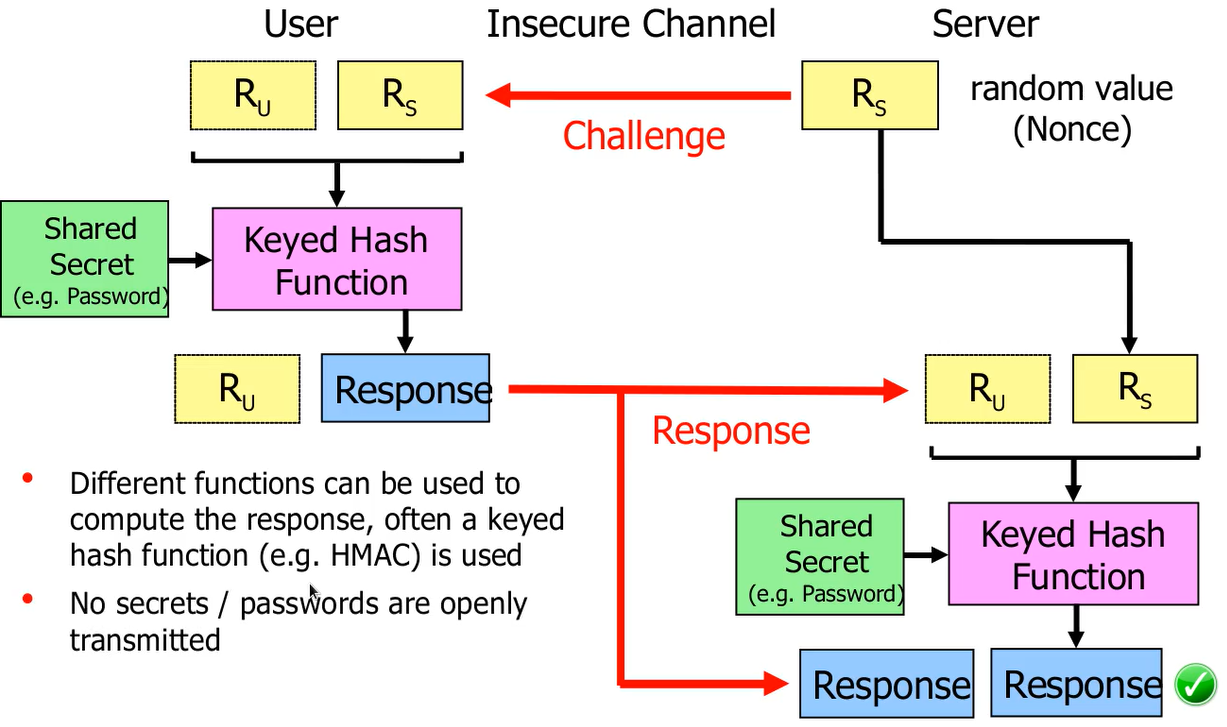
\includegraphics[width=150px]{img/CRPSharedSecret.png}
	\captionof{figure}{Challenge-Response Protocols with Shared Secrets}
	\label{fig:Challenge-Response Protocols with Shared Secrets}
\end{Figure}

\begin{Figure}
\centering
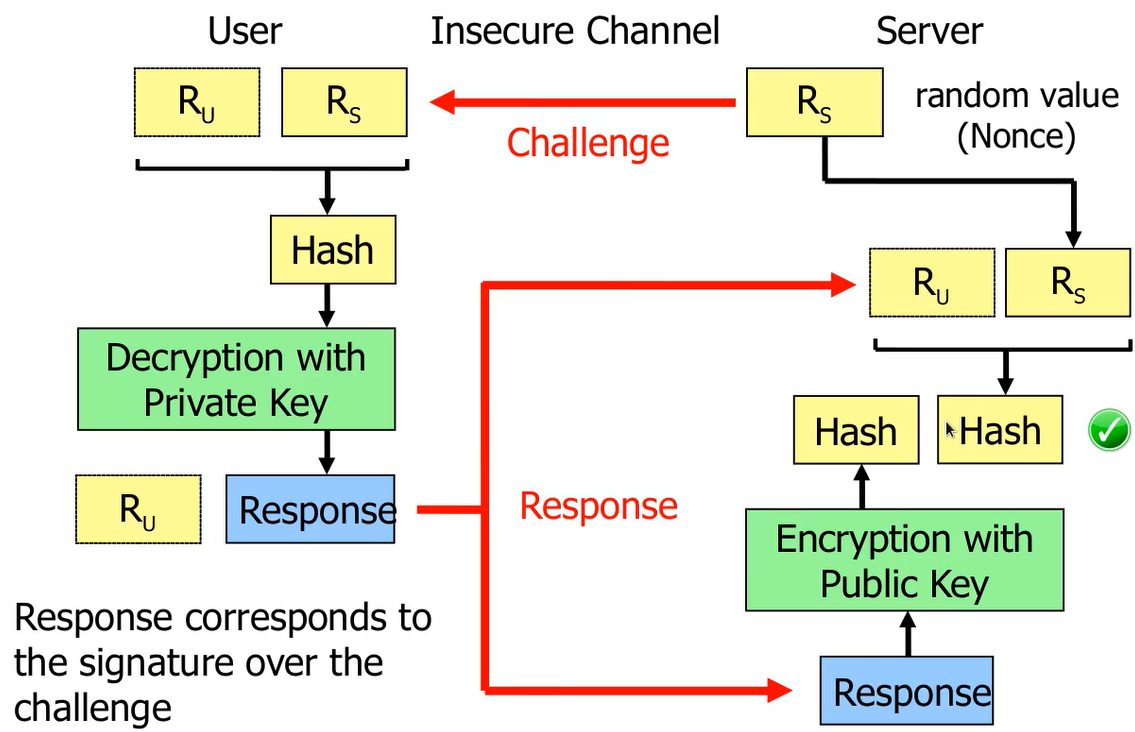
\includegraphics[width=150px]{img/CRPDigitalSignature.png}
	\captionof{figure}{Challenge-Response Protocols with Digital Signature}
	\label{fig:Challenge-Response Protocols with Digital Signature}
\end{Figure}

	\subsection{Cracking Password used in Challenge-Response Protocol}
\begin{itemize}
	\item \textbf{Online Attack}: Der Angreifer probiert unterschiedliche Passwörter direkt beim Service aus, was jedoch sehr unwahrscheinlich ist, da es immer eine neue Challenge gibt
	\item \textbf{Offline Attack}: Ich zeichne erfolgreiche Authentifikationen auf und probiere nun vers. Passwörter in die keyed hash function zu stecken um die korrekte Response zu erhalten.
\end{itemize}
$\Rightarrow$ Auch hier kann Key-Streching ausgeführt werden um das Leben des Angreifers zu erschweren

\chapter{Vorlesung 6 - Sichere Kommunikation mit Fokus auf Layer 2}

\section{Sie kennen was mit sicheren Kommunikationsprotokoll erreicht und nicht erreicht werden kann}
	\subsection{Grundlegendes}
Die fundementalen Internet Protokollen (IP, TCP, etc) stellen keine Sicherheitsmassnahmen zur Verfügung\\
Daraus resultieren verschiedene Gefahren in der Internet-Kommunikation
\begin{itemize}
	\item Eavesdropping $\rightarrow$ Lesen von Daten bei der Übermittlung
	\item Manipulating Data $\rightarrow$ Ändern von Daten bei der Übermittlung
	\item Injecting Data $\rightarrow$ Hinzufügen von Daten bei einer bestehenden Kommunikationsbeziehung
	\item Replaying Data $\rightarrow$ Wiederversenden von bereits gesendeten Daten
	\item Getting unauthorised access $\rightarrow$ die Verwendung eines Systems ohne Privilegien, z.B. nach der Erlangung von Berechtigungsnachweisen durch Lauschangriff
	\item Masquerading $\rightarrow$ Vorgaukeln, dass man eine andere Person oder System ist
\end{itemize}

	\subsection{Hauptziel der sicheren Kommunikation}
	Um diese Ziele zu erreichen, werden kryptografische Protokolle eingesetzt
	\begin{itemize}
		\item Confidentiality $\rightarrow$ Nur der Empfänger der Kommunikation kann die Daten Lesen
		\item Integrity $\rightarrow$ Der Empfänger kann feststellen, falls Daten manipuliert wurden
		\item Authenticity $\rightarrow$ Das Vorgaukeln, dass man jemand anders ist, kann nicht passieren
	\end{itemize}
		\subsubsection{Minor Goals - werden selten gefordert}
	\begin{itemize}
		\item Non-Repudiation $\rightarrow$ Der Empfänger kann nicht vernein, dass er Daten erhalten bzw. versendet hat
		\item Anonymity $\rightarrow$ Der Empfänger (oder auch Sender) können sich gegenseitig nicht identifzieren
	\end{itemize}

	\subsection{Limitationen von Sicherheitsprotokollen}
	\begin{itemize}
		\item Software Schwachstellen werden dadurch nicht geschützt
		\item Schützt einem nicht vor Malware
		\item Schützt einem nicht vor DoS Attacken
	\end{itemize}
	$\Rightarrow$ Da die Sicherheitsprotokolle zunehmend komplexer werden (Implementation oder Protokoll Unschönheiten), sind diese insicher jenachdem unsicher $\rightarrow$ in der Regel sollten keine eigenen Sicherheitsprotokolle geschrieben werden

\section{Sie verstehen weshalb die sichere Kommunikation auf verschiedenen OSI-Layer stattfindet und haben einen Überblick über die verschiedenen Protokollen auf den verschiedenen Layern}


	\begin{itemize}
		\item Die Protokolle kommen auf allen unterschiedlichen Layern zum Einsatz, je nach Anwendungsgebiet
		\item Typerischerweise ist die Implementation auf den höheren Layern einfacher, je höher im Layer, desto spezifischer für einen konkreten Anwendungsfall
		\item Auf den tieferen Layern, braucht man häufig noch die Absicherung von Hardware-Geräten, kann viel allgemeiner eingesetzt werden
	\end{itemize}

\begin{Figure}
\centering
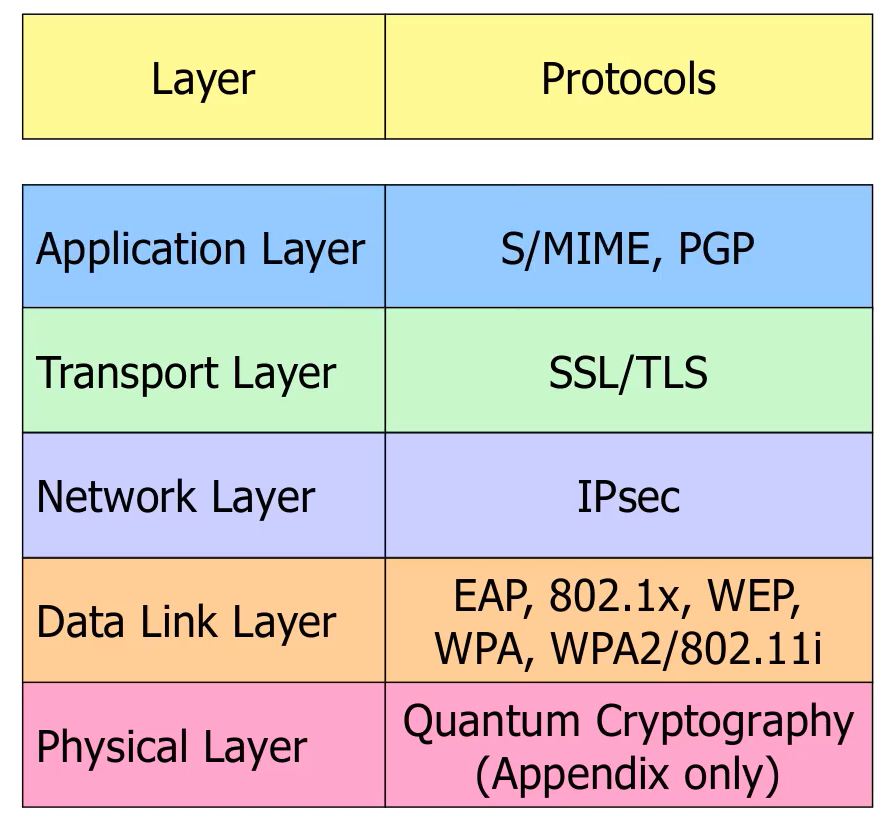
\includegraphics[width=150px]{img/ProtocolPerLayer.png}
	\captionof{figure}{Überblick über die verschiedenen Protokollen pro Layer}
	\label{fig:Überblick über die verschiedenen Protokollen pro Layer}
\end{Figure}


\section{Sie verstehen die erweiterbare Authenifzierungsprotokolle und wie diese nach dem IEEE 802.1x Standard funktionieren, allen vor an für Portbasierte Netzwerkzugriffskontrolle aktivieren}
\begin{itemize}
	\item Die Verschlüsselung auf Layer 2 haben bei draht-Verbindungen haben fast keine Singifikanz
	\item Jedoch ist eine hohe Singifikanz spannend bei der draht- / sowie drahtlosen Verbindung betrf. der Authentifikation $\rightarrow$ Exentsible Authentication Protocol (EAP), wobei EAP weder eine Authentifikation, noch eine erweiterbare Möglichkeit anbieten (hat daher eine falschen Namen erhalten)
\end{itemize}

	\subsection{EAP}
\textbf{Wichtig:} EAP ist weder ein Protokoll noch erweiterbar $\rightarrow$ es ist mehr eine Art und Weise wie Nachrichten verpackt werden
\begin{itemize}
	\item Ein EAP-Paket packt andere Protokolle ein
	\item ist mehr ein Standard
	\item hat 50 unterschiedliche Authentifkation Methoden $\rightarrow$ wird im Type-Field festgelegt
\end{itemize}

	Darauf aufbauend gibt es nun \textit{IEEE802.1x: Port-based Network Access Control} $\rightarrow$ eines der wichtigsten Anwendungen von EAP\\
	\begin{itemize}
		\item LAN-Ports sind nicht per Default nicht offen
		\item Bevor dieser Port geöffnet wird, muss diese Connection authenifiziert werden
		\item Dabei wird EAP als Authentifizierungsprotokoll verwendet
		\item IEEE 802.1x definiert wie EAP die Nachricht enkapsuliert innerhalb des Ethernet / WLAN-Frames $\rightarrow$ EAP over LAN (EAPOL)
	\end{itemize}
\begin{Figure}
\centering
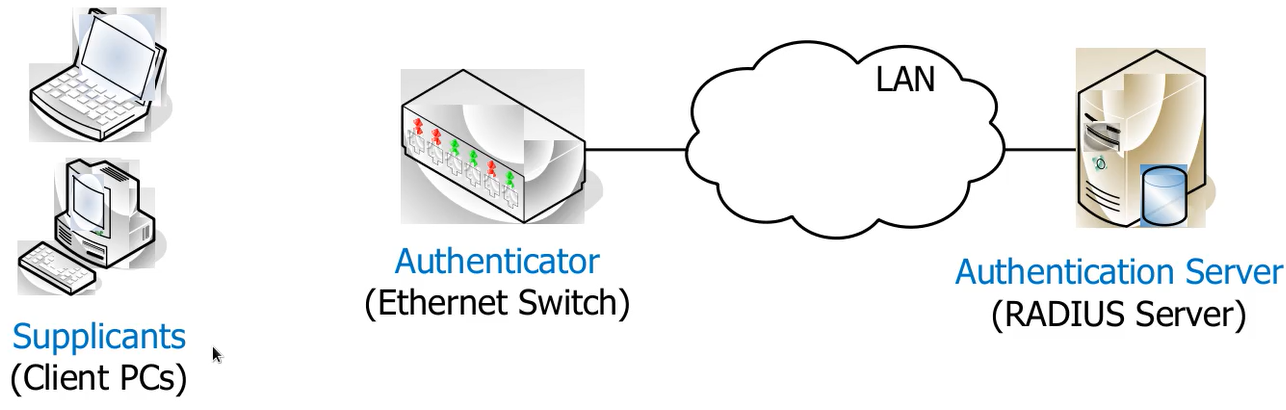
\includegraphics[width=150px]{img/EAPSchema.png}
	\captionof{figure}{Schema bei einem IEEE802.1x Aufbau}
	\label{fig:Schema bei einem IEEE802.1x Aufbau}
\end{Figure}

	\subsection{IEEE 802.1x mit EAP-TLS Authentikation}
Dabei wir jeder Nachricht einfach mit dem EAP eingepackt inkl. dem TLS-Handshake
\begin{Figure}
\centering
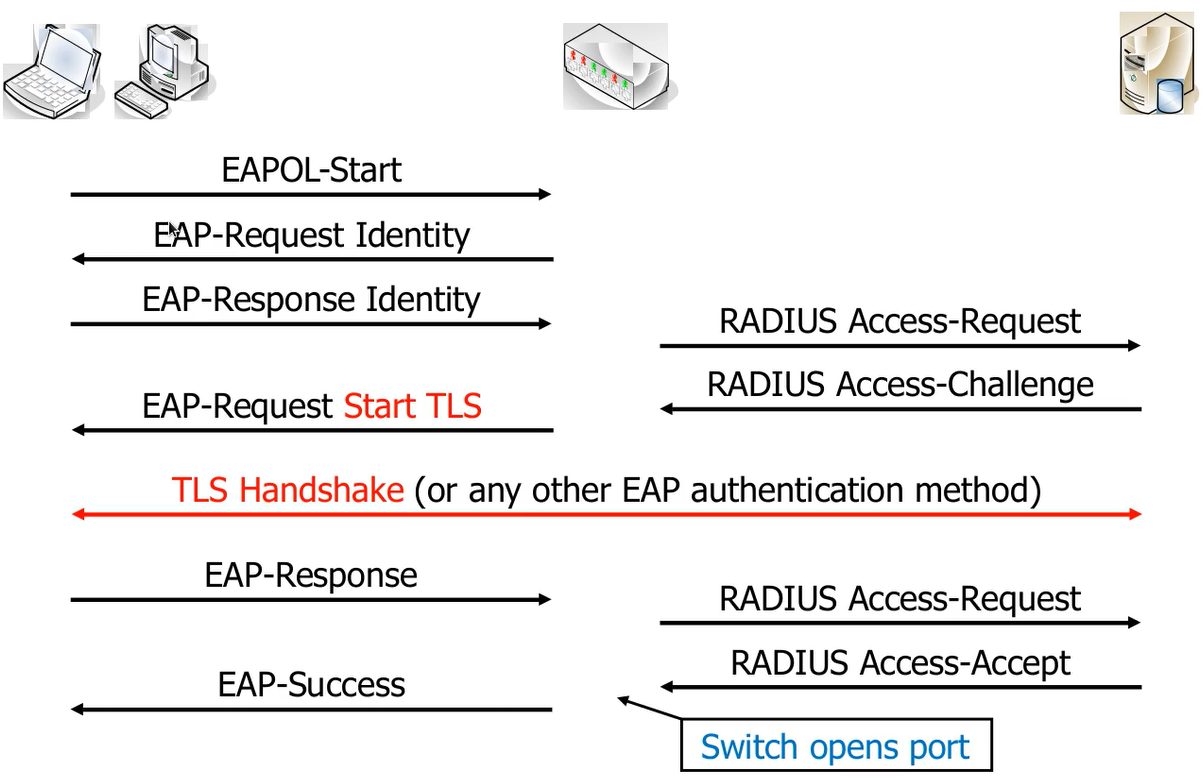
\includegraphics[width=150px]{img/EAPTLS.png}
	\captionof{figure}{Nachrichtenverlauf eines IEEE 802.1x mit EAP-TLS Authentikation}
	\label{fig:Nachrichtenverlauf eines IEEE 802.1x mit EAP-TLS Authentikation}
\end{Figure}
Für den Switch sind einzig die RADIUS-Nachrichten von Relevanz, vor allem die RADIUS Access-Accept $\rightarrow$ anschliessend wird der Port geöffnet

\section{Sie verstehen die Funktionalität der verschiedenen Sicherheitsmechanismen für WLAN und können die Sicherheitseigenschaften und -probleme erläutern}
	\subsection{Security of WLAN}
\begin{itemize}
	\item Es ist kein Kabel vorhanden, so kann jeder in der Nähe solche Pakete abfangen / sniffen $\rightarrow$ Pakete müssen verschlüsselt werden
	\item Nur gewisse Personen sollen Zugriff haben
	\item Dies soll alles auf dem Layer 2 geschehen, so dass jeder Datenaustausch zwischen Clients und Access-Point geschützt ist
	\item IEEE 802.11i (auch bekannt unter WPA2) as the official successor of WEP (Wired Equivalent Privacy)
	\item Es gibt immer noch eine wenige Access-Points welche offen sind
\end{itemize}
	
	\subsection{WLAN Sicherheit mit Wired Equivalent Privacy (WEP)}
\begin{itemize}
	\item Access-Point und alle Clients teilen sich um einen vorkonfigurierten Langzeit-Schlüssel
	\item Dieser Schlüssel wird für das verschlüsseln der einzelnen Frames verwendet $\rightarrow$ Alle Clients nutzen den selben Key und können somit den Datentransfer von allen Clients mitlesen.
	\item Die Länge des Schlüssels ist entweder 40 oder 104 Bits mit der RC4-Verschlüsselung $\rightarrow$ erreichen sicherlich nicht den gewünschten Workfactor, des Weiteren wird RC4 als geknackt gekennzeichnet
\end{itemize}

		\subsubsection{Frame Protection}
Für jeden individuellen Frame, passiert folgendes:
\begin{Figure}
\centering
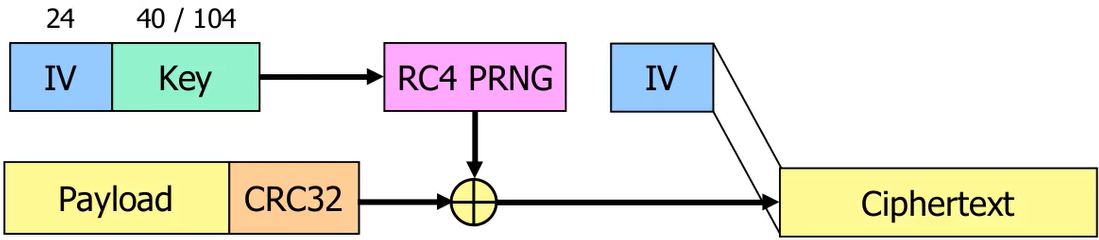
\includegraphics[width=150px]{img/FrameProtection.png}
	\captionof{figure}{Frame Protection}
	\label{fig:Frame Protection}
\end{Figure}

\begin{itemize}
	\item CRC Checksume schützt die payload Integrität
	\item 40-Bits SChlüssel sind eine schlechte Wahl
	\item 104-Bits grundsätzlich gut, jedoch immer noch nicht total sicher
	\item Grund dafür spätestens nach $2^24$ wiederholt sich der Schlüssel nochmals $\rightarrow$ wir attackieren nicht den Schlüssel, sondern die verschiedenen Keystreams
\end{itemize}

		\subsubsection{erster Angriff}
Wir sniffen alle Frames und warten bis der IV sich wiederholt $\rightarrow$ bei zufälligem IV geschieht dies nach 4'823 Frames (Birthday Paradox), schliemmsten Fall muss man alle $2^24$ abwarten.\\
Wenn man zwei Ciphertext mit dem gleichen IV ermittelt hat, kann man folgendes durchführen:
\begin{Figure}
\centering
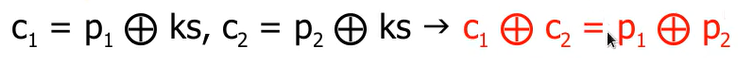
\includegraphics[width=150px]{img/FormelIV.png}
	\captionof{figure}{Die Formel für das Erkennen des Ciphertexts}
	\label{fig:Die Formel für das Erkennen des Ciphertexts}
\end{Figure}
$\Rightarrow$ Durch den Plaintext erhalten wir in aller Regel viel mehr Struktur (bspw. Englischer-Text oder TCP-Paket). Daraus kann man dann sämtliche Keystreams ausrechnen $\rightarrow$ Jedoch hat man dann mit ein paar wenigen 100 GBs die Möglichkeit sämtliche Texte zu entschlüssel ohne, dass man den Schlüssel kennt.

		\subsubsection{zweiter Angriff}
Angriff auf die Schwachstellen von RC4
\begin{itemize}
	\item Wenn man nur eine kleine Anzahl von Bits kennt, kann man den Keystream mit einer Wsk von 50 Prozent vorhersagen
	\item WEP verwendet IV, dadurch kennen wir schon die ersten 24 Bits des RC4 Keys
\end{itemize}
$\Rightarrow$ WEB ist total unsicher

		\subsubsection{Warum ist CRC kein guter MAC}
\begin{itemize}
	\item Nur Verschlüsselung ist keine gute Wahl und sollte mit Integrität-Schutz erweitert werden
	\item WEP stellt ein verschlüsselter CRC zur Verfügung, was jedoch nciht von allen Attacken schützt
\end{itemize}

	\subsection{Wi-Fi Protected Access}
Der neue Standard von IEEE ging so lange, dass sich eine Gewerkschaft mit der Lösung auseinandersetzte.\\
Die Client-Authentifikation kann auf zwei Möglichkeiten stattfinden:
\begin{itemize}
	\item Port-based Network access control gemäss IEEE 802.1x
	\item Pre-shared Key (PSK) $\rightarrow$ Vor allem zuhause, wenn man das WLAN-PW verteilt
\end{itemize}

Der Client und den Access-Point wird richtig verschlüsselt:
\begin{itemize}
	\item zwei 128-Bit unicast keys für die Verschlüsselung und Integritätsschutz (eindeutig pro Client und Session)
	\item zwei 128-bit broadcast keys für die Verschlüsselung und Integritätsschutz (gleich für alle Clients)
	\item periodic re-keying, normalerweise gibt es nach einer Stunde einen neuen Schlüssel
\end{itemize}

Beide Standards definieren zwei Verschlüsselungs-Modes $\rightarrow$ TKIP und CCMP\\
\textbf{Temporal Key Integrity Protocol (TKIP)}:  tbd
\textbf{CCMP}: tbd

		\subsubsection{TKIP Security}
\begin{itemize}
	\item den Einsatz von MAC für den Integritätsschutz ist eine gute Idee
	\item TKIP verwendet jedoch immer noch den RC4-Alogrithmus
	\item TKIP verwendet Michael als MAC-Alogrithmus
\end{itemize}

		\subsubsection{CCMP Security}
\textbf{Counter Mode CBC-MAC Protocol}
\begin{itemize}
	\item WPA/WPA2 verwendet CCMP mit AES und 128-Bits Key
	\item WPA2 unterstützt immer CCMP
	\item Aktuell ist noch keine Unsicherheit betreffend CCMP
\end{itemize}

\begin{Figure}
\centering
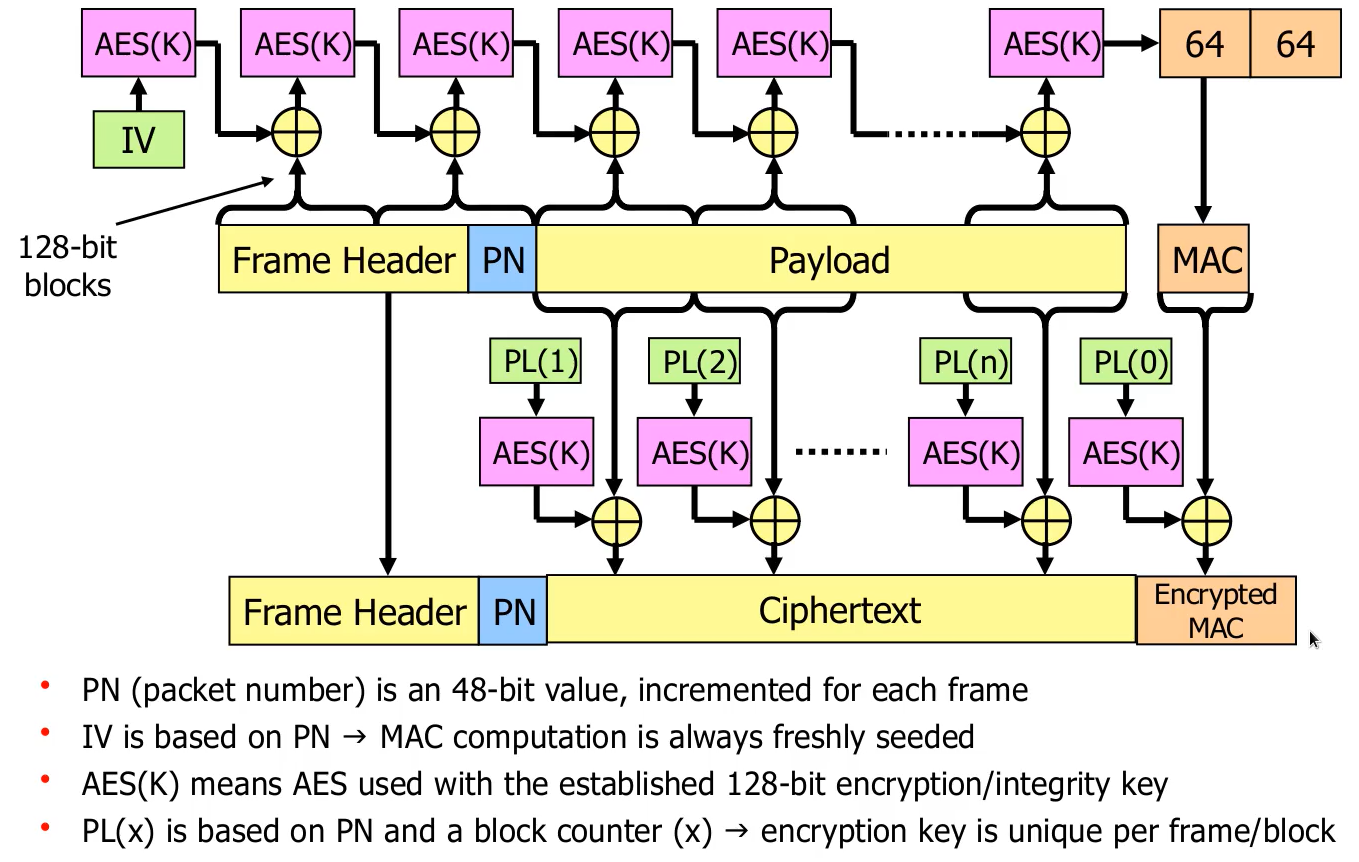
\includegraphics[width=150px]{img/CCMPSecurity.png}
	\captionof{figure}{Ablauf von CCMP}
	\label{fig:Ablauf von CCMP}
\end{Figure}


\chapter{Vorlesung 7 - Firewalls}

\section{Sie wissen was eine Firewall ist, und was sie (nicht) kann}
\begin{itemize}
	\item Eine Firewall ist ein Netzwerkgeräte, welche zwischen zwei oder mehreren Netzwerken kontrolliert
	\item Die Firewall ist immer auch ein Router, welcher die Pakete weiterleitet
	\item Grundlage hierfür ist eine Security Police
	\item Basierend auf der Security Police, wird eine oder mehrere Firewalls installiert	
\end{itemize} 

\textbf{Was kann man machen?}
\begin{itemize}
	\item Zugriff kontrollieren auf die verschiedenen Internet-Seiten
	\item Zugriff kontrollieren vom Internet auf die internen Computer und Services
	\item Bösartigen Traffic unterbinden (bspw. HTTP-Traffic für SQL-Injection)
	\item Einer der wichtigsten Komponenten
	\item Blockieren von nicht-gewollten-Traffic
	\item Struktur von Aussen verstecken
\end{itemize}

\textbf{Wozu nicht?}
\begin{itemize}
	\item Teilt implizit die Welt in Innen und Aussen auf, solange die Angreifer von Aussen sind, funktioniert. Sobald sie im Inneren des Netzwerk sind, schützen sie nicht mehr
	\item Schützt sie nicht vor Attacken auf dem Applikation Layer
\end{itemize}


\section{Sie verstehen den Unterschied zwischen packet-filtering firewalls und application layer firewalls and wissen den grundsätzlichen Einsatz von beiden Typen}
$\Rightarrow$ In der Praxis verwendet man beide Arten der Firewalls um eine möglichst gute Sicherheit zu gewährleisten
	\subsection{packet-filtering firewalls}
\begin{itemize}
	\item meist genutzte Typ
	\item operiert auf dem Network-Layer (manchmal auch auf den Transport-Layer)
	\item Die Firewall erhält ein Paket und bevor es zum anderen Netzwerk weitergeleitet wird, begutachtet es das Paket
	\item end-to-end Kommunikation wird nicht aufgespalten
	\item meistens werden die headers inspiziert 
	\item \textit{Beispiel} Erlaube jedem Host im Netzwerk 160.85.37.0/24 mit Host 160.85.215.20 zu kommunizieren, dies jedoch nur über Port 80
	\item \textbf{Vorteil} Sehr schnell, da es nur den Layer 3 und 4 die Protokol-Header überprüft werden muss
	\item \textbf{Limitationen} Man kann nur beschränkten, wer mit wem reden kann - jedoch kann man den Inhalt, welcher kommuniziert wird, nicht beschränken
	\item Gibt viele kommerzielle Produkte auf dem Markt
\end{itemize}
	
		\subsubsection{Einsatzgebiet}
\textbf{Szenario I:}\\
\begin{itemize}
	\item Firewall hat drei Netzwerk Interfaces, drei Netzwerke
	\item Internes Netzwerk mit Computern und internen Services (print server, file server etc.)
	\item Demilitarized Zone (DMZ) mit public services (web, email etc.)
	\item externes Netzwerk, alles andere
	\item \textbf{Vorteil} Nur eine Firewall notwendig
	\item \textbf{Nachteil} Firewall ist single point of failure und ein Angreifer muss nur eine Firewall überwinden
\end{itemize}
\begin{Figure}
\centering
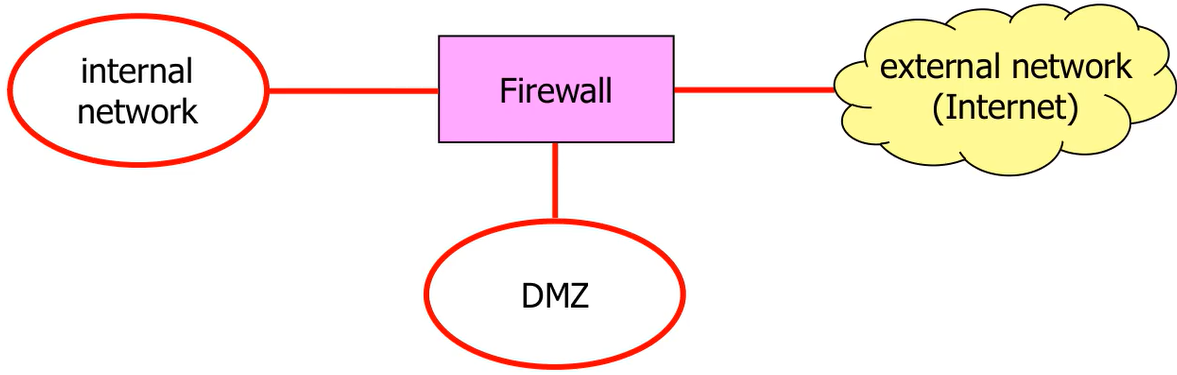
\includegraphics[width=150px]{img/PacketFilteringI.png}
	\captionof{figure}{Schema des ersten Packet Filterin Szenario}
	\label{fig:Schema des ersten Packet Filterin Szenario}
\end{Figure}

\textbf{Szenario II:}\\
\begin{itemize}
	\item Zwei Firewall, mit jeweils zwei Netzwerk interfaces, immer noch drei Netzwerk
	\item DMZ wird auf zwei Firewalls aufgeteilt
	\item \textbf{Vorteile}: Zwei Firewalls (idealerweise von unterschiedlichen Herstellern) vom externen zum internen Netzwerk
	\item \textbf{Nachteile}: Teurer und es braucht mehr Expertise für die Konfiguration
\end{itemize}
\begin{Figure}
\centering
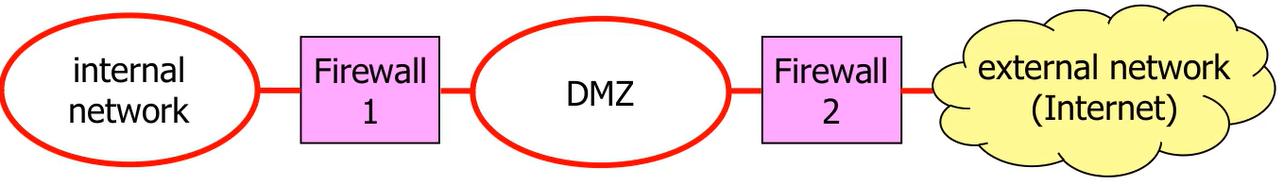
\includegraphics[width=150px]{img/PacketFilteringII.png}
	\captionof{figure}{Schema des zweiten Packet Filterin Szenario}
	\label{fig:Schema des zweiten Packet Filterin Szenario}
\end{Figure}
		
	\subsection{application layer firewalls}
\begin{itemize}
	\item Arbeitet auf dem Application Layer (oft auch Web-Applikation oder Proxy Firewall) $\rightarrow$ wird oft verwendet um die Webseite zu schützen
	\item spaltet die End-To-End-Kommunikation
	\item Inspektiert application layer daten gemäss den Regeln, sofern die Daten i.O. sind, wird es weitergeleitet
	\item \textit{Beispiel} Überprüfen, ob HTTP-Request JavaScript-Code enthält und falls dem der Fall ist, dies blockieren
	\item \textbf{Vorteil} Man hat deep inspection für alle Daten die ausgetauscht werden
	\item \textbf{Limitationen} Relativ langsam, es gibt Schwierigkeiten für verschlüsselte Daten, Normalerweise für einen Typ von Applikation
\end{itemize}

		\subsubsection{Einsatzgebiet}
\textbf{Web Application Firewall (WAF)}:
\begin{itemize}
	\item zwei Firewalls mit drei Netzwerken
	\item um den Zugriff auf den Webserver(mit Weltkugel) zu reglementieren, wird FW2 verwendet um nur HTTP-Request für die WAF zuzulassen
	\item DNS muss so konfiguriert dass die Namensauflösung auf die WAF zeigt
	\item Zugriff vom externen ins interne Netzwerk wird mittels den blauen Linien dargestellt
\end{itemize}



\section{Sie verstehen den Unterschied zwischen stateless und statefull firewalls}

	\subsection{stateless Firewalls}
\begin{itemize}
	\item Jedes IP-Paket wird komplett isoliert von allen anderen behandelt
	\item die Firewall merkt sich nicht welche Verbindungen bestehen
	\item \textbf{Nachteil:} Firewalls sind meistens offener als man es braucht, nur sehr eingeschränkten Support für komplexe Protokolle (bspw. FTP)
\end{itemize}

	\subsection{Stateful Firewalls}
\begin{itemize}
	\item heutzutage sind beinahe alle Firewalls statefull
	\item Firewall merkt sich ob bestimmte Pakete zu bestimmten Sessions gehören
	\item typische Informationen: Protokoll, source und destination der IP-Adresse, Ports, Sessiondauer, Protokol-Phase (TCP)
	\item \textbf{Vorteile} Braucht weniger Regel (ca. die Hälfte), Return-traffic wird nur noch on-demand erlaubt, Support für komplexe Protokolle (bspw. FTP)
	\item netfilter und nftables unterstützt Stateful Packet-Filtering
\end{itemize}


\section{Sie kennen das fundamentale Konzept von der netfilter/nftables-Architektur und können nftables anwenden um eine einfache Firewall zu konfigurieren}
\textbf{netfilter} ist ein uralters Programm, welches sehr viele Möglichkeiten bietet:
\begin{itemize}
	\item Erlaubt Packet-Filtering
	\item Erlaubt Network Adress Translation (NAT)
	\item erlaubt general packet mangling
	\item ist ein Mechanismus der den Zugriff auf die Pakete erlaubt und diese entsprechend analysiert, modifiziert, extrahiert oder löscht
\end{itemize}

\textbf{nftables} ist ein darauf aufbauendes Netzwerk Klassifizierungs-Tool
\begin{itemize}
	\item Packet-Filtering Firewall kann damit implementiert werden
	\item Network Address Translation kann damit realisiert werden
\end{itemize}

\textbf{nft} ist der Name des Command Line Tools um nftables zu konfigurieren

	\subsection{Linux Netfilter}
\begin{itemize}
	\item der Kernel hat eine bestimmte Anzahl an Hooks, welche an unterschiedliche Punkte zum Zuge kommt
	\item bspw. vor dem INGRESS oder nach dem POSTROUTING, des Weiteren bei INPUT und OUTPUT
\end{itemize}

Es gibt gesamthaft acht Hooks:
\begin{enumerate}
	\item INGRESS, da kommt da Paket frisch von der Netzwerkkarte
	\item PREROUTING, Paket wurde entgegengenommen und Checksummen wurden geprüft aber noch keine Verarbeitung (ist noch nicht klar, ob das Paket an ein anderes Netzwerk weitergeleitet oder intern verwendet)
	\item INPUT, falls bei der Routing Decision entschieden wird, dass das Paket für den lokalen Zweck ist
	\item FORWARD, falls bei der Routing Decision entschieden wird, dass das Paket für ein anderes Paket notwendig ist
	\item POSTROUTING, das Paket wird an die Netzwerkkarte ausgeliefert
	\item OUTPUT, kommt vom lokalen Prozess und geht an die Netzwerkkarte
\end{enumerate}

\begin{Figure}
\centering
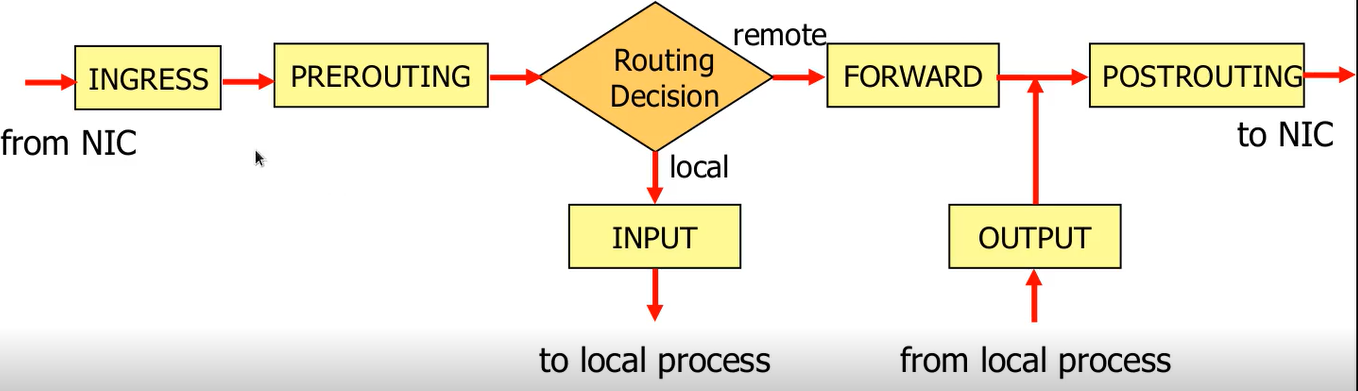
\includegraphics[width=150px]{img/netfilterHooks.png}
	\captionof{figure}{Die 8 Hooks beim Netfilter}
	\label{fig:Die 8 Hooks beim Netfilter}
\end{Figure}

	\subsection{nftables Rules}
\begin{itemize}
	\item nftables Regeln haben einen Classification Part und einen oder mehrere Action-Parts
	\item \textbf{Classification:} Auf welche Pakete soll diese Regel angewendet werden
	\item \textbf{Action:} Sagt was mit diesen Pakete gemacht werden soll
	\item accept-Action die Verarbeitung des Paket wird weitergeführt
	\item drop-Action Die Verarbeitung wurde gestoppt, jedoch wird auch nichts damit gemacht, sprich der Sender erhält keine Mitteilung
	\item reject-Action Verarbeitung des Pakets wurde gestopppt, sender erhält eine Meldung mittels ICMP-Paket $\rightarrow$ Standardtext \textit{port unreachable}, diese Nachricht kann auch noch angepasst werden bspw. durch \textit{... reject with icmp type host-prohibited}
	\item jump-Action Man möchte die Verarbeitung eines Pakets an einer anderen Stelle fortsetzen
	\item (häufige) Empfehlung bei Pakete welche man nicht verwenden möchte sollte man drop verwenden $\rightarrow$ Angreifer erkennen auch bei Drop, dass es eine Firewall gibt
	\item Sysadmin möchten jedoch eine Antwort erhalten und daher ist die drop dann nicht 
	\item ip steht für IPv4 Pakete
	\item ip6 steht für IPv6
	\item daddr steht für destination adress
\end{itemize}

\textbf{Beispiel Befehle}
\begin{itemize}
	\item \textit{ip daddr 8.8.8.8 drop} $\rightarrow$ sämtliche Bedienungen müssen eintreffen, dass sie zum Zuge kommen
	\item \textit{ip6 nexthdr tcp accept} $\rightarrow$ akzeptiert alle IPv6 Pakete mit einem TCP Header
	\item \textit{ip6 nexthdr != tcp accept}
	\item \textit{iifname eth2 accept} $\rightarrow$ Akzeptiert alle Pakete welche vom interface eth2 kommen
	\item \textit{icmp type echo-request limit rate 10/second accept} $\rightarrow$ Maximal 10 ICMP echo-request (ping) limitieren
\end{itemize}

	\subsection{nftables chain}
\begin{itemize}
	\item Regeln sind in Chains organisiert
	\item Base-chain in der Table gibt es einen Hook
	\item non-base-chain nicht mit einem Hook
	\item Classification wird von open nach unten durchgeführt, bis eine Regel ausgeführt. Sobald eine zutrifft, werden die anderen nicht ausgeführt
	\item Falls keine Regel zutrifft, dann kommt eine policy zum Zuge
	\item default-policy ist accept
	\item Chains haben einen Typ, hier verwenden wir grundsätzlich \textit{filter}
	\item Chains haben auch eine entsprechende Prioritäten
\end{itemize}

\textbf{Beispiel:}\\
chain ssh-traffic {
\t type filter hook input priority 0; policy drop;\\
\t tcp dport ssh count accept
}

\begin{itemize}
	\item \textit{type filter}: Chain wird für Paket-Filtering verwendet
	\item \textit{hook input}: ist zum INPUT-hook angegliedert (base chain)
	\item \textit{priority 0}: hat die Priorität 0 (mittlerer Wert)
	\item \textit{policy drop}: unklassifizierte Pakete werden gedropped
\end{itemize}
$\Rightarrow$ Nur Pakete an SSH

	\subsection{nftables Tables}
\begin{itemize}
	\item chains werden in TABLES zusammengefasst
	\item Tables fassen alle Chains der gleichen Art zusammengefasse
	\item diese Paket-Tyoes werden auch Adress families genannt (ip = nur IPv4; ip6 = nur IPv6; inet = IPv4 und IPv6)
\end{itemize}

	\subsection{nftables Ruleset and Scripting}
\begin{Figure}
\centering
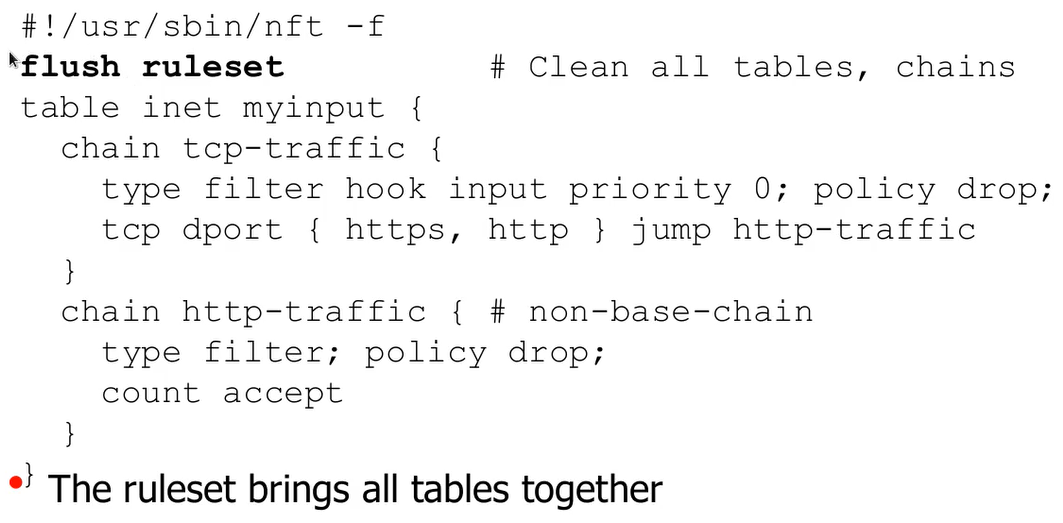
\includegraphics[width=150px]{img/nftablesRuleset.png}
	\captionof{figure}{Beispielcode eines Rulesets}
	\label{fig:Beispielcode eines Rulesets}
\end{Figure}

\begin{itemize}
	\item \textit{\#\!/usr/sbin/nft -f} wird für die Ausführung verwendet
	\item File soll ausführbar sein
	\item es gilt eine atomare Ausführung (entweder es wird alles ausgeführt oder nichts)
	\item \textit{flush ruleset} gesamte Ruleset wird atomar ersetzt
	\item mittels \textit{define} können Variable definiert werden, diese können dann im Code mittels \$ + Variablenname verwendet werden
\end{itemize}

	\subsection{Vorgehen beim Aufbau eines nftables}
\begin{enumerate}
	\item Belegung von Variablen mittels \textit{define}. Dabei haben wir die präfixe i für internes Netzwerk, d für DMZ, e für externes Netzwerk. Postfix ifc für interface, net für Netzwerk, addr = Addreess des Interfaces Richtung Firewall
	\item INPUT, OUTPUT und FORWARD Hooks muss je eine Chain erarbeitet werden (myinput, myforward, myoutput) das gesamte resultiert in der table myfilter; Alle policies sind drop.
\end{enumerate}

\section{Sie verstehen die Absicht eines Port-Scanners und können diesen mittels port scan und nmap anwenden und interpretieren}
\begin{itemize}
	\item Ist eine Technik um herauszufinden welche Dienste auf einem Remote-Dienst alles laufen
	\item wird häufig von Angreifer verwendet um sich einen ersten Überblick zu verschaffen
	\item Man überprüft ob der Host verfügbar ist (Ping)
	\item Aufbauen einer TCP Verbindung, falls das funktioniert handelt es sich um einen offenen Port. Bei einer TCP RST Antwort handelt es sich um einen geschlossenen Map
	\item populärster Port-Scanner ist nmap
\end{itemize}

\textbf{Beispiel nmap}\\
Überprüfen ob der TCP Port 80 bei der ZHAW offen ist: \textit{nmap -80 www.zhaw.ch}\\
\begin{Figure}
\centering
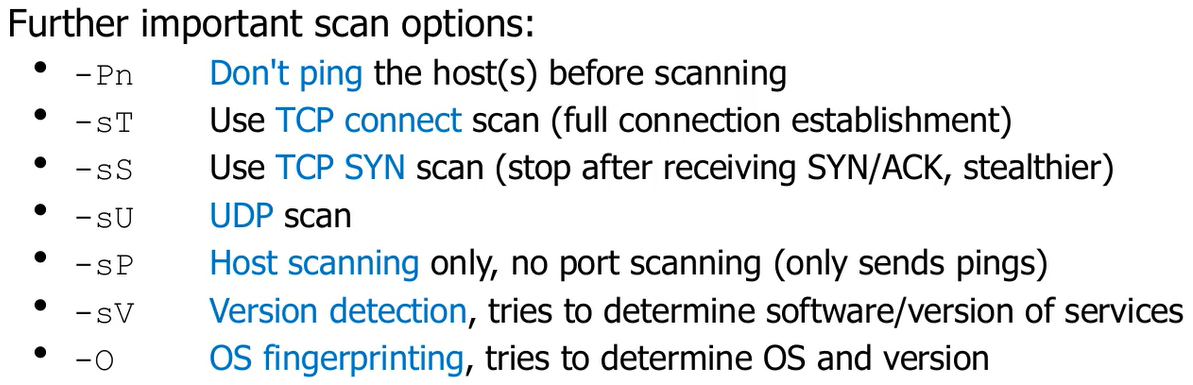
\includegraphics[width=150px]{img/nmapCommand.png}
	\captionof{figure}{Weitere Befehle bei nmap}
	\label{fig:Weitere Befehle bei nmap}
\end{Figure}

\chapter{Vorlesung 8 - end-to-end Communication}

\section{Sie verstehen was end-to-end communication security bedeutet}
\begin{itemize}
	\item Schutz zwischen zwei Endanwendungen oder zwei Anwendungen
	\item Zwischenstellen sehen nur verschlüsselte Daten und sehen nie eine Nachricht im Klartext
	\item Protokolle werden auf Layer 3 oder höher implementiert (nur da ist End to End Verschlüsselung möglich)
	\item TLS (Layer 4)
	\item IPSec (Layer 3)
\end{itemize}

\section{Sie verstehen das TLS Protokoll}

\begin{itemize}
	\item TLS ist für das \textbf{s} in https zuständig
	\item Vorgänger war SSL
	\item stellen eine End-to-End Kommunikation zwischen zwei Applikationen zur Verfügung
	\item TLS1.3 ist am kommen, aber TLS1.2 ist noch die dominierende Version
	\item TLS für authentication, Integritätsschutz, Vertraulichkeit
\end{itemize} 

\begin{itemize}
	\item Web (HTTP)
	\item Mail (POP3 / IMAP)
	\item Mail Server (SMTP)
	\item File up- / download
\end{itemize}

\begin{itemize}
	\item Ist auf dem TCP-Layer aufbauend
	\item TLS kann direkt im User space (Applikation mittels Library) implementiert werden

\end{itemize}

\begin{Figure}
\centering
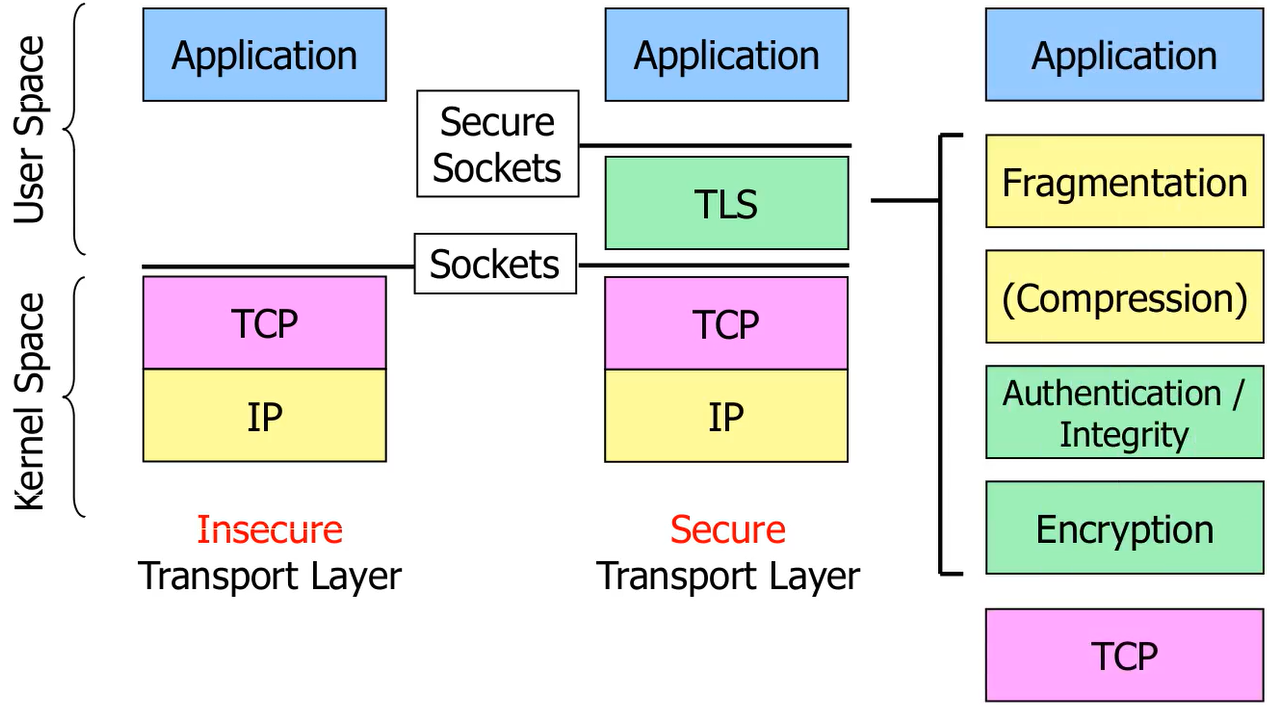
\includegraphics[width=150px]{img/TLSProtocolStack.png}
	\captionof{figure}{Abbildung des Protokoll Stacks in TLS}
	\label{fig:Abbildung des Protokoll Stacks in TLS}
\end{Figure}
$\Rightarrow$ TCP/IP haben wir immer!

\begin{Figure}
\centering
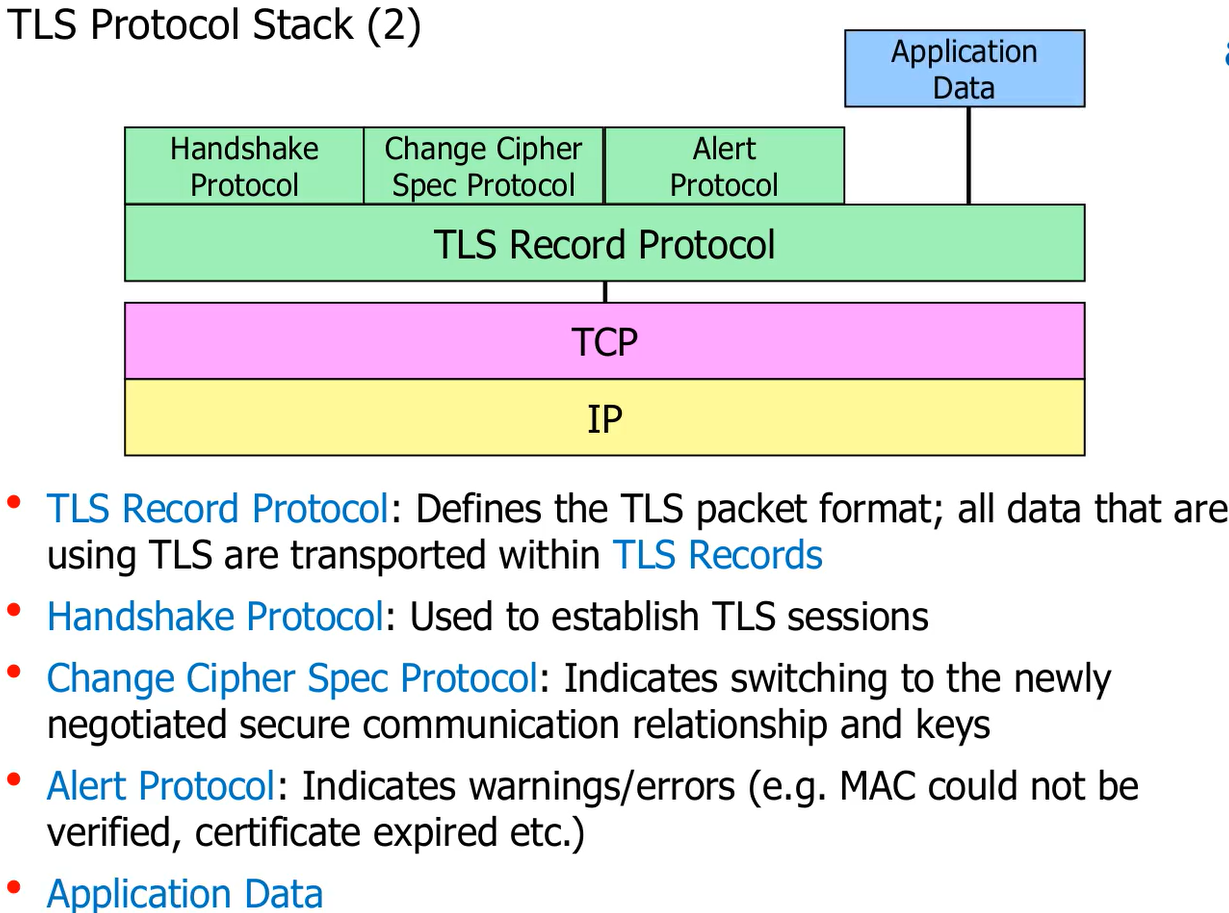
\includegraphics[width=150px]{img/TLSProtocolStackII.png}
	\captionof{figure}{Abbildung des Protokoll Stacks in TLS}
	\label{fig:Abbildung des Protokoll Stacks in TLS}
\end{Figure}
$\rightarrow$ Wir beschäftigen uns mit dem blauen Teil, der grüne Teil kommt durch die Library

\begin{Figure}
\centering
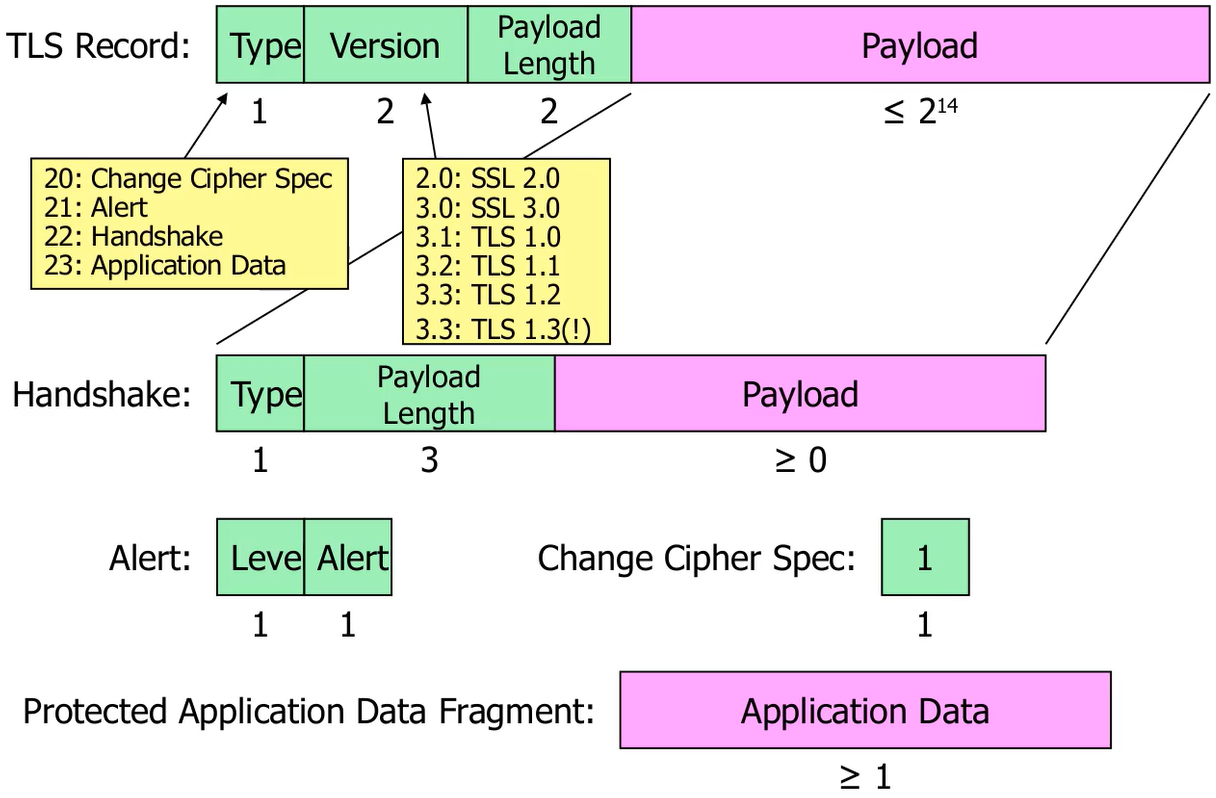
\includegraphics[width=150px]{img/TLSMessageFormats.png}
	\captionof{figure}{Abbildung der verschiedenen Formatmöglichkeiten}
	\label{fig:Abbildung der verschiedenen Formatmöglichkeiten}
\end{Figure}

	\subsection{sie können erklären wie ein TLS Handshake funktioniert}
Man nimmt an, es gibt bereits eine valide TCP Verbindung (SYN, SYNACK, ACK $\rightarrow$ three-handshake ist durch) $\rightarrow$ Zu diesem Zeitpunkt gibt es noch keinen Schutz.\\

Grundsätzlicher Ablauf
\begin{enumerate}
	\item Client schickt an Server eine \textit{ClientHello}-Nachricht
	\item Server schickt an Client \textit{ServerHello} $\rightarrow$ je nach vereinbarte Methode schickt \textit{Zertifikat*, Schlüsselaustausch* und eine Zertifikat-Anfrage*} $\rightarrow$ \textit{ServerHelloDone}-Nachricht sobald der Server fertig ist $\Rightarrow$ Durch TCP kommt es auf die richtige Abfolge draufan
	\item Client erzeugt \textit{Session-Keys}
	\item Client schickt die notwendige Informationen an den Server für den Abschluss des Handshakes (Clientseitig) $\rightarrow$ Client schickt noch eine ChangeCipherSpec um mitzuteilen, dass genügend Informationen vorhanden sind um die Daten zu verschlüsseln $\rightarrow$ Finished-Nachricht um die nicht verschlüsselten Daten im Nachhinein zu authentifzieren
	\item Server erzeugt \texit{Session-Keys} $\Rightarrow$ Wenn alles richtig gelaufen ist, haben Client und Server die gleichen Session-Keys
	\item Server sendet ChangeCipherSpec und Finished-Nachricht an den Client
\end{enumerate}
\begin{Figure}
\centering
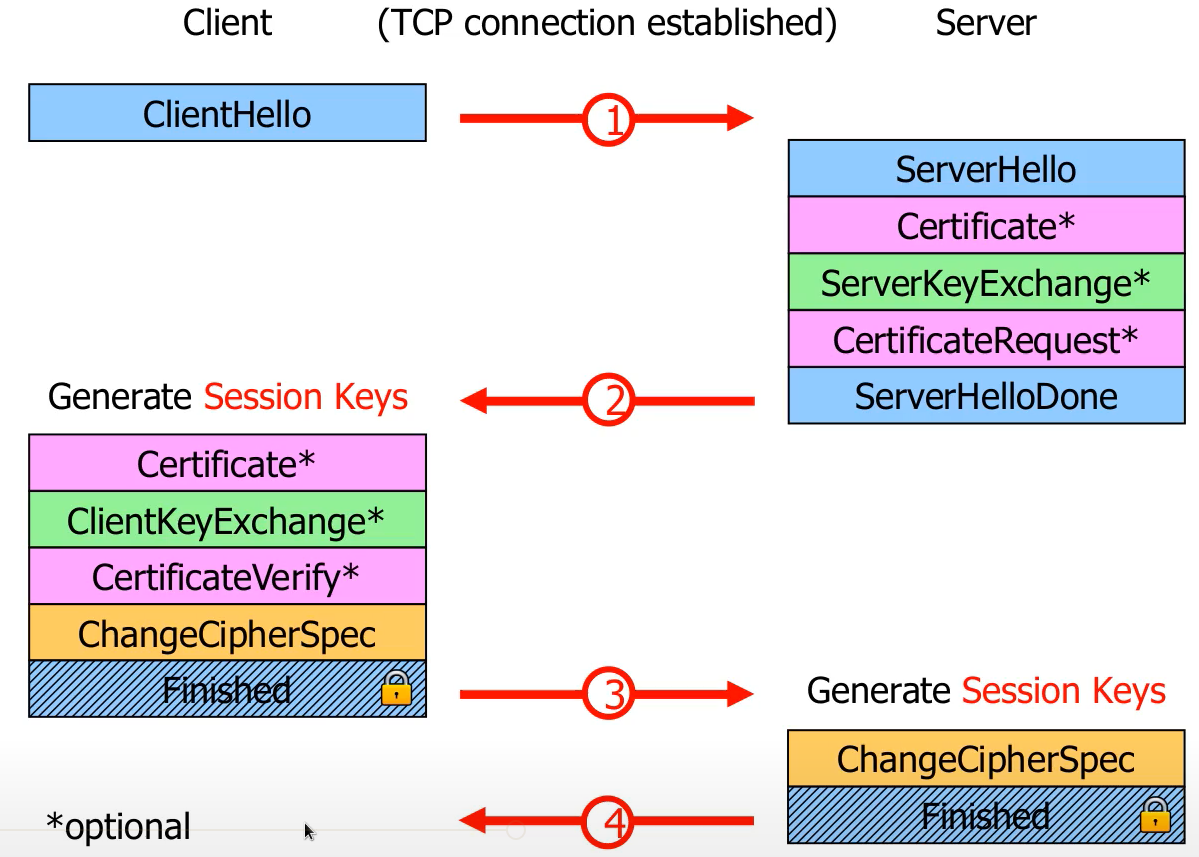
\includegraphics[width=150px]{img/TLSHandshake.png}
	\captionof{figure}{Abbildung des Ablaufs eines TLS Handshakes}
	\label{fig:Abbildung des Ablaufs eines TLS Handshakes}
\end{Figure}

\textbf{Beispiel TLS 1.2 Handshake mittels RSA Key Exchange, Server-side Authentication}
\begin{Figure}
\centering
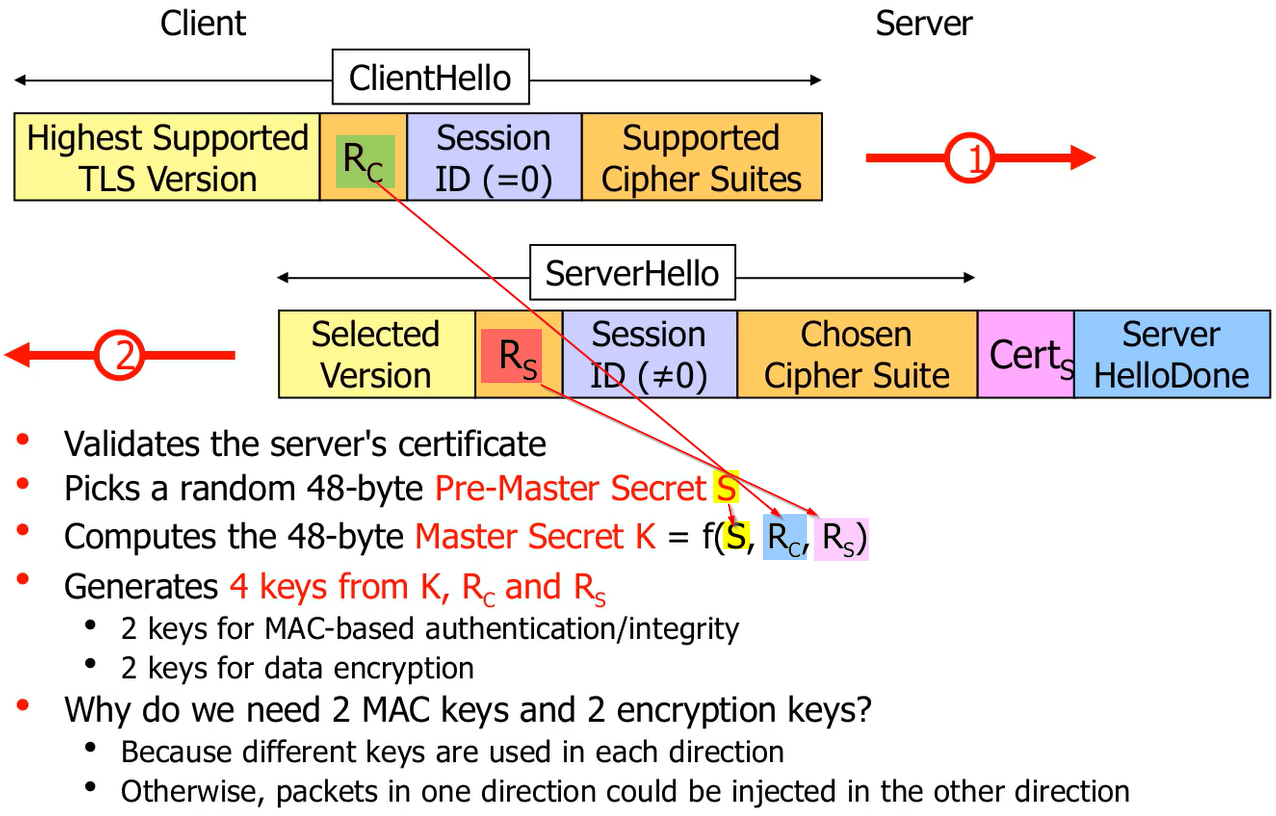
\includegraphics[width=150px]{img/TLSHandshakeRSA.png}
	\captionof{figure}{Abbildung des Ablaufs eines TLS Handshakes mittels RSA Key Exchange (1)}
	\label{fig:Abbildung des Ablaufs eines TLS Handshakes mittels RSA Key Exchange (1)}
\end{Figure}

\begin{Figure}
\centering
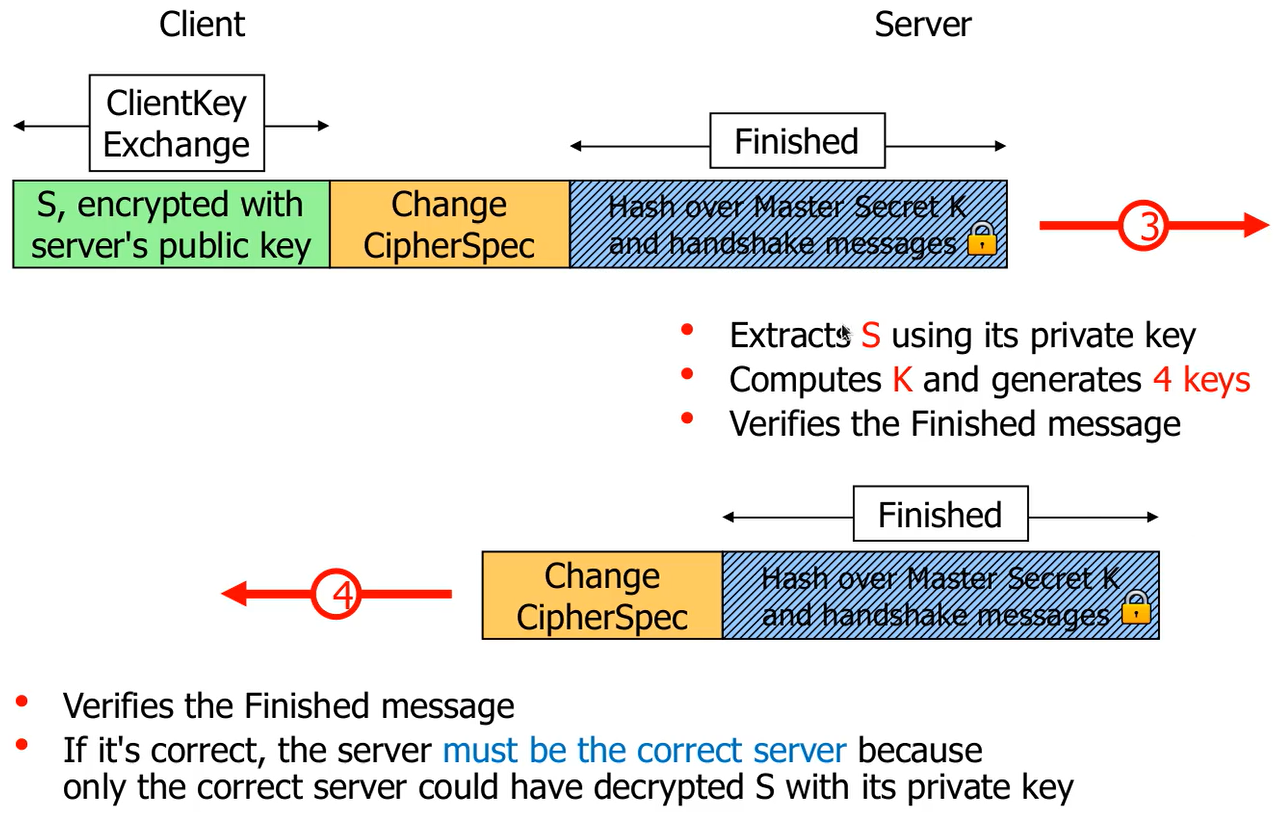
\includegraphics[width=150px]{img/TLSHandshakeRSAII.png}
	\captionof{figure}{Abbildung des Ablaufs eines TLS Handshakes mittels RSA Key Exchange (2)}
	\label{fig:Abbildung des Ablaufs eines TLS Handshakes mittels RSA Key Exchange (2)}
\end{Figure}

\textbf{Beispiel TLS 1.2 Handshake mittels Diffie-Hellman Key Exchange, Server-side Authentication}
\begin{Figure}
\centering
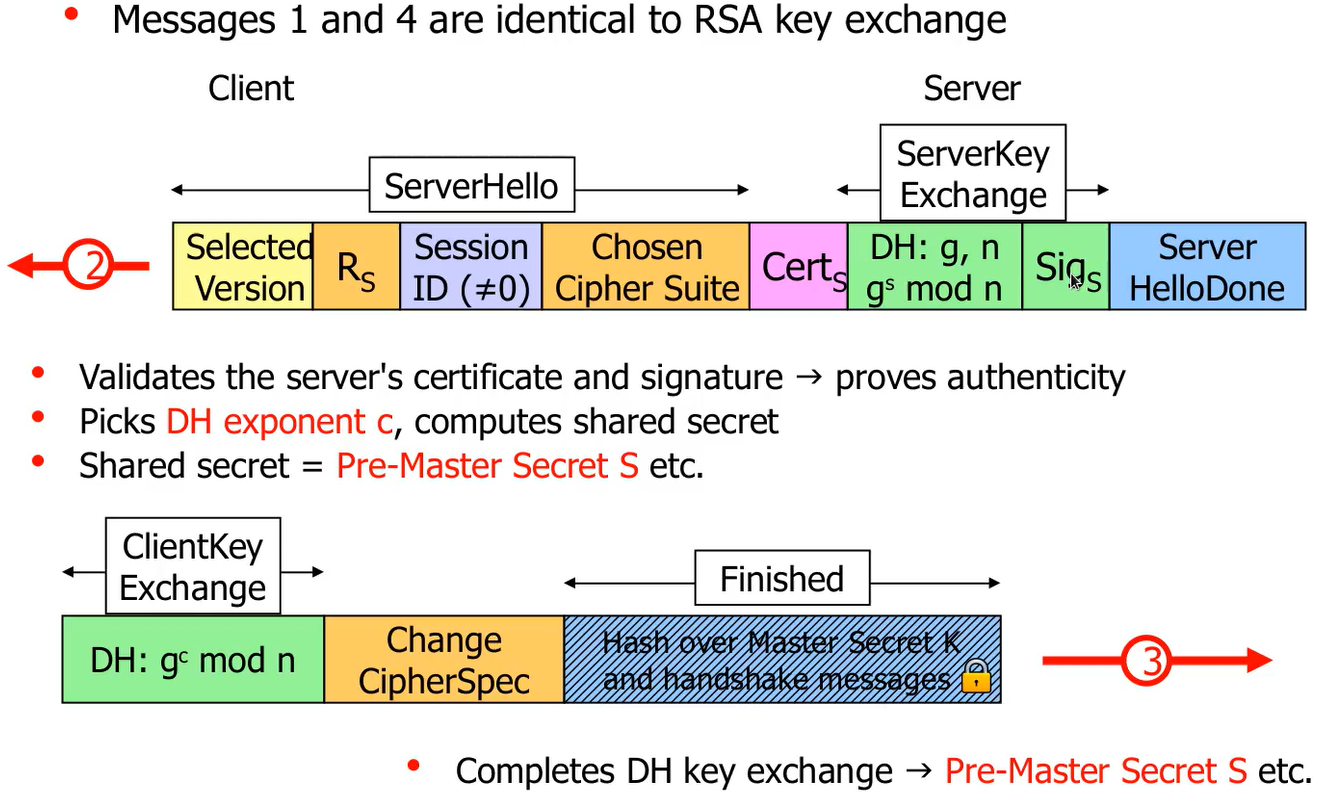
\includegraphics[width=150px]{img/TLSHandshakeDiffieHellman.png}
	\captionof{figure}{Abbildung des Ablaufs eines TLS Handshakes mittels Diffie-Hellman Key Exchange (2)}
	\label{fig:Abbildung des Ablaufs eines TLS Handshakes mittels Diffie-Hellman Key Exchange (2)}
\end{Figure}

\textbf{Beispiel TLS 1.2 Handshake Additional Client-side Authentication}
\begin{Figure}
\centering
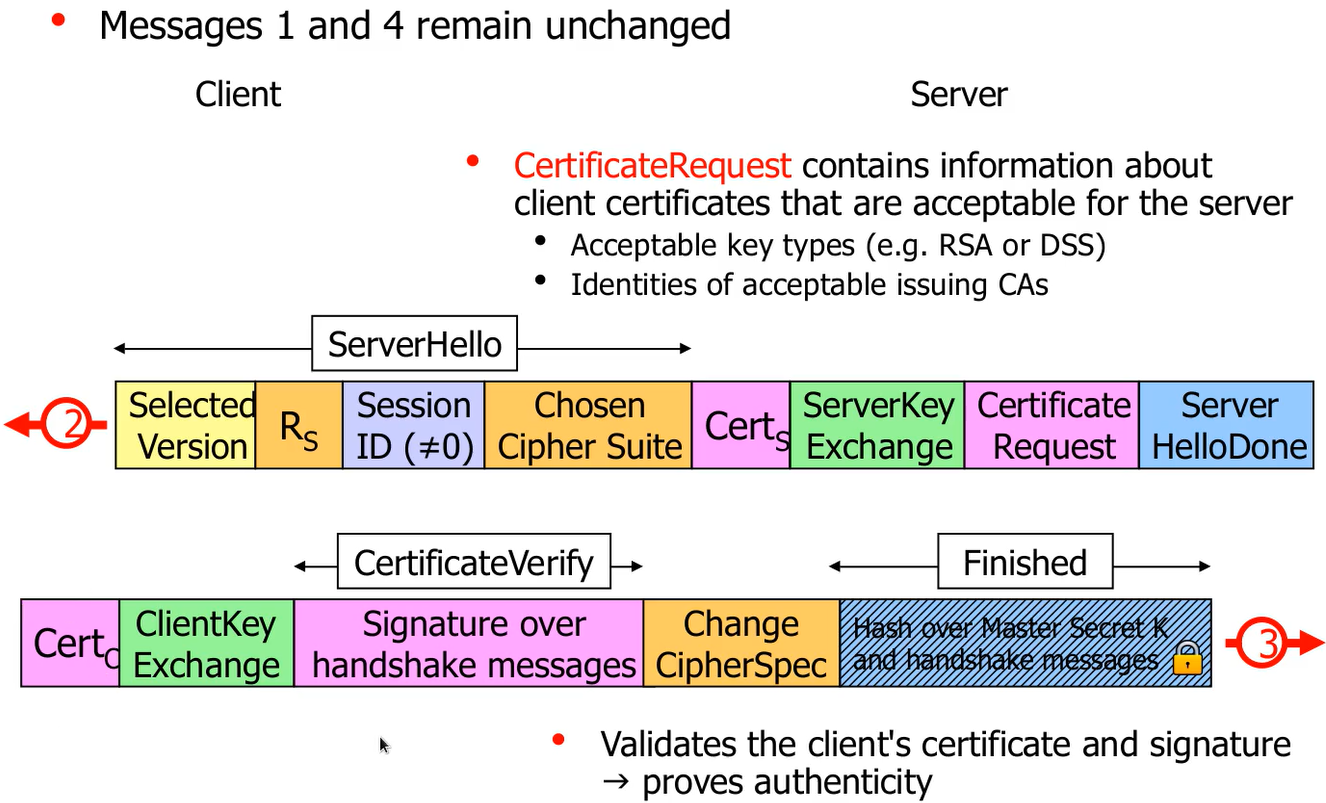
\includegraphics[width=150px]{img/TLSHandshakeClientSide.png}
	\captionof{figure}{Abbildung des Ablaufs eines TLS Handshakes client-side Authentication}
	\label{fig:Abbildung des Ablaufs eines TLS Handshakes client-side Authentication}
\end{Figure}

	\subsection{Sie wissen wir Applikationsdaten mittels TLS-Protokoll ausgetauscht werden}
\begin{itemize}
	\item Client und Server sind im Besitz der 4 Schlüssel
	\item Nun erfolgt der Datenaustausch
\end{itemize}

Annahme: Man verwendet Block-Cipher im CBC-Mode

\begin{Figure}
\centering
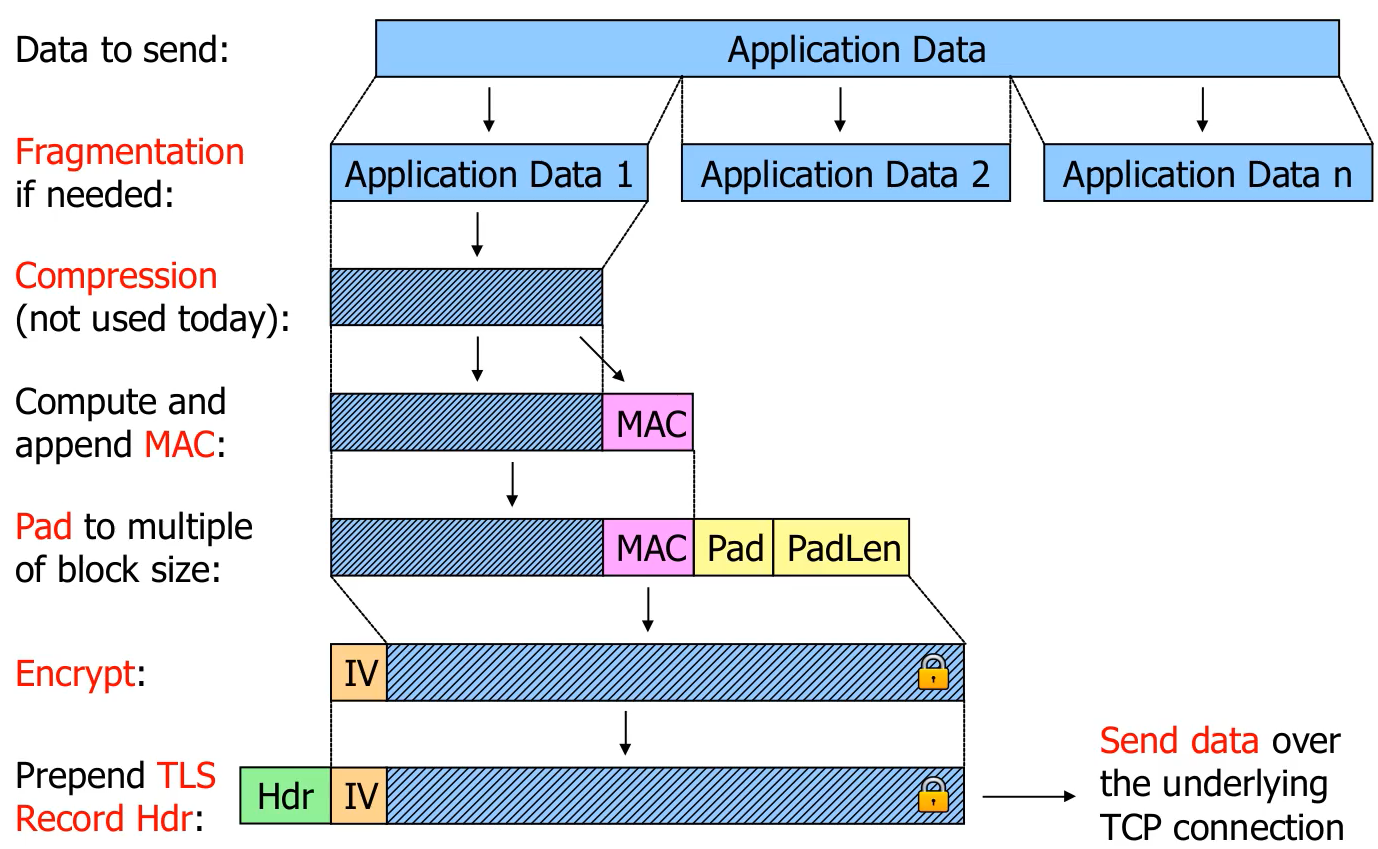
\includegraphics[width=150px]{img/TLSSendingData.png}
	\captionof{figure}{Abbildung des Ablaufs eines TLS Dataaustausch}
	\label{fig:Abbildung des Ablaufs eines TLS Dataaustausch}
\end{Figure}
$\Rightarrow$ TCP-Verbindung, ist nicht Paketorientiert sondern ein Stream $\rightarrow$ TCP garantiert, dass die Pakete in der richtigen Reihenfolge ankommen\\

%ToDo Truncation Attack Vorlesung S.31 ergänzen
in a nutshell: Man sendet vor dem Beenden eine Nachricht \texit{Ich beende jetzt die Verbindung, ich habe alles übertragen}

	\subsection{Sie können erklären wie TLS die Authentification, Integritätsschutz und Confidentiality zur Verfügung stellt}
%ToDo
	
	\subsection{Sie kennen das Basisprinzip von wie Schlüsselmaterial erstellt wird}
\textbf{1. Schritt}:
\begin{itemize}
	\item Das \texit{Pre-Master Secret} wird im Vorfeld berechnet und das \textit{Master Secret} (Server) ist auf jeden Fall 48 Byte lang 
	\item zusätzlich kommt nun noch ein \textit{Seed} (besteht aus Master Secret, $R_c$ und $R_s$), falls aus Zufallsgründen das Pre-Master Secret auf beiden Seite gleich irgendeinmal gleich sein sollte, das Master-Secret trotzdem noch verschieden ist durch den Einsatz von $R_c$ bzw. $R_s$
\end{itemize}

\begin{Figure}
\centering
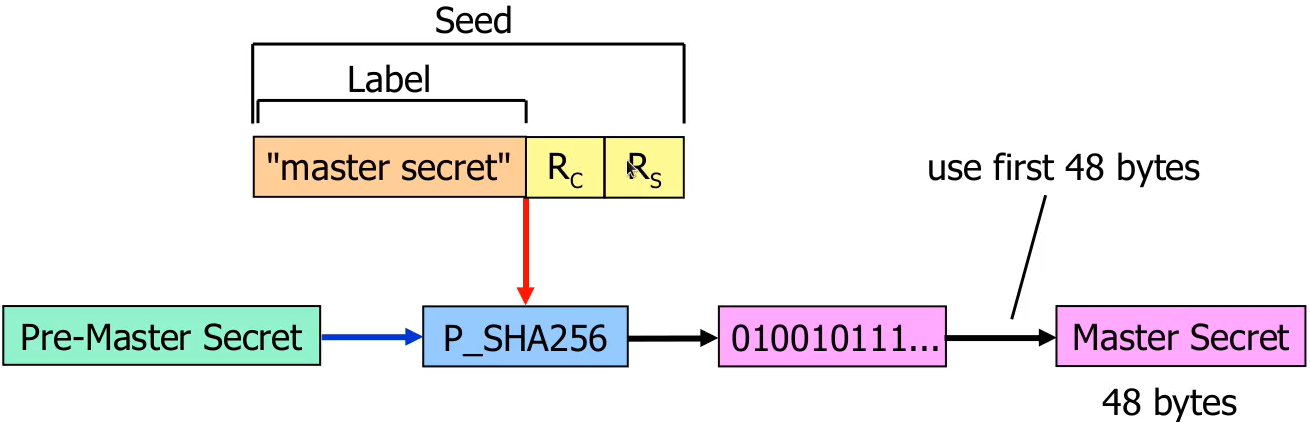
\includegraphics[width=150px]{img/MasterSecretStepI.png}
	\captionof{figure}{Abbildung des ersten Schrittes in der Berechnung des Master Secrets}
	\label{fig:Abbildung des ersten Schrittes in der Berechnung des Master Secrets}
\end{Figure}

\textbf{2. Schritt}
\begin{itemize}
	\item Das Key Material hat unbestimmte Länge an Bytes $\rightarrow$ man verwendet dann die ersten n Bytes (ist abhängig von dem Verfahren)
	\item ebenfalls ein Seed im Einsatz (Jedoch ein anderer!)
\end{itemize}

\section{Sie kennen den aktuellen Stand von TLS und seinem Vorgänger SSL in Bezug auf die Sicherheit und wissen, welche Versionen auf sichere Weise verwendet werden können}
\begin{itemize}
	\item SSL1.0 und SSL2.0 unsicher 
	\item SSL3.0 und TLS1.0 wurde seit September 2011 als knackbar dargestellt
	\item $\rightarrow$ alte TLS Versionen vor allem TLS1.0 nicht mehr unterstützen!
	\item SSL2.0/3.0 wird immer noch unterstützt $\rightarrow$ sehr schlecht!
	\item Die unsicheren Versionen unteranderem TLS1.0 wird immernoch von 65\% der Websiten-Server unterstützt
	\item TLS1.2 (Standard) wird von 95\% der Website-Server unterstützt
	\item TLS1.3 kommt immer mehr
	\item Firefox unterstützt alle sichere Versionen
	\item in der neusten Firefox Version ist TLS1.0/1.1 per default disabled
\end{itemize}

\begin{Figure}
\centering
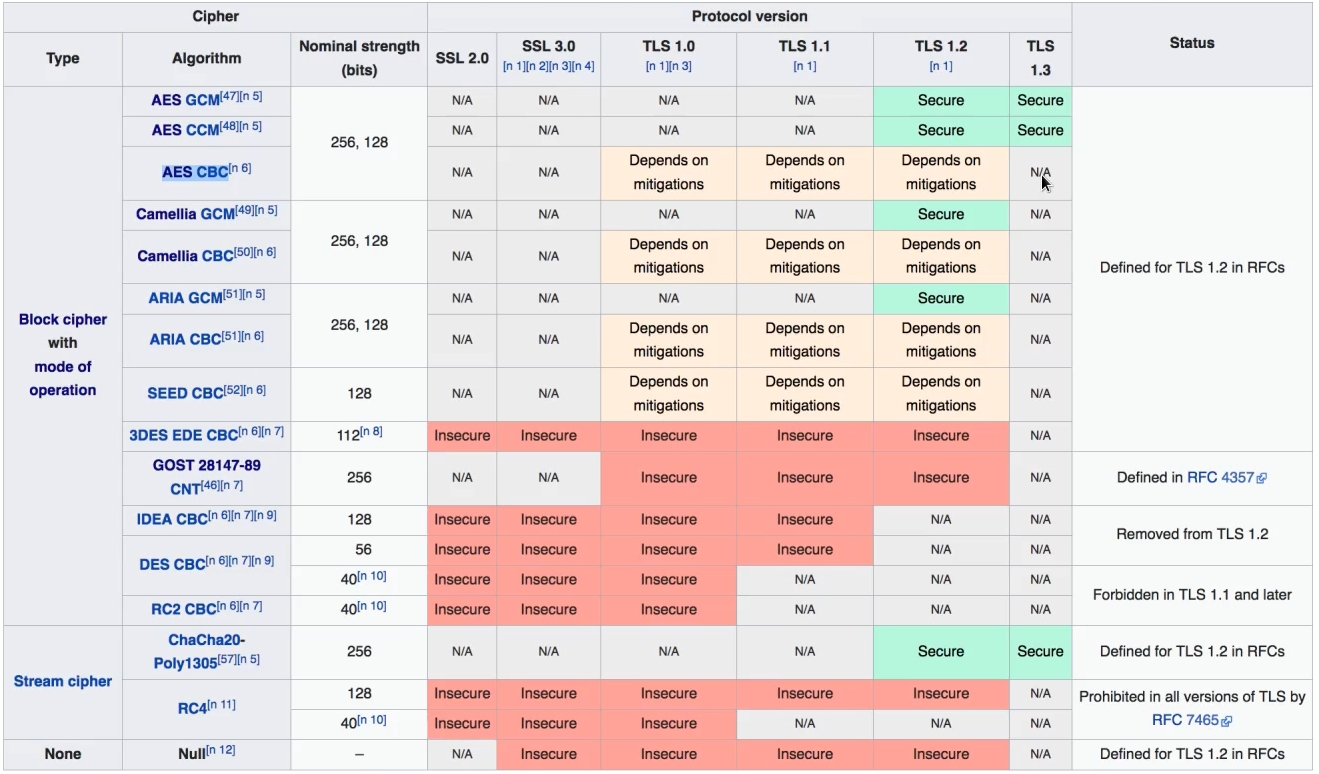
\includegraphics[width=150px]{img/TLSVersions.png}
	\captionof{figure}{Abbildung aktueller Stand des Sicherheitsstandards}
	\label{fig:Abbildung aktueller Stand des Sicherheitsstandards}
\end{Figure}

\section{Sie verstehe die Basis Funktion von IPsec und können die Eigenschaften im Vergleich zu TLS vergleichen}
\begin{itemize}
	\item Sichere End-to-End Kommunikation auf dem Netzwerklayer (Layer3)
	\item Sicherung von IP packet payload und teile des IP headers
	\item Confidentiality, authentication, integrity ist gewährleistet
	\item definierter Schlüsselaustausch mittels Internet Key Exchange (IKE)
	\item IPSec muss im Kernel der Endpunkte installiert sein
	\item Schützt die Pakete (unabhängig der Anwendung) zwischen zwei Hosts
	\item Vorteil: Automatisch alle Daten und Protokoll oberhalb des Layer3 geschützt werden
\end{itemize}

Bei IPSec gibt es zwei unterschiedliche Modi:
\begin{itemize}
	\item Authentication Header $\rightarrow$ authenticated and integrity Protected $\Rightarrow$ Macht wenig sinn ohne Verschlüsselung
	\item Encapsulating Security Payload (ESP) $\rightarrow$ encypted, authenticated and integrity protected $\Rightarrow$ einzig relevanter Modi
\end{itemize}

\begin{Figure}
\centering
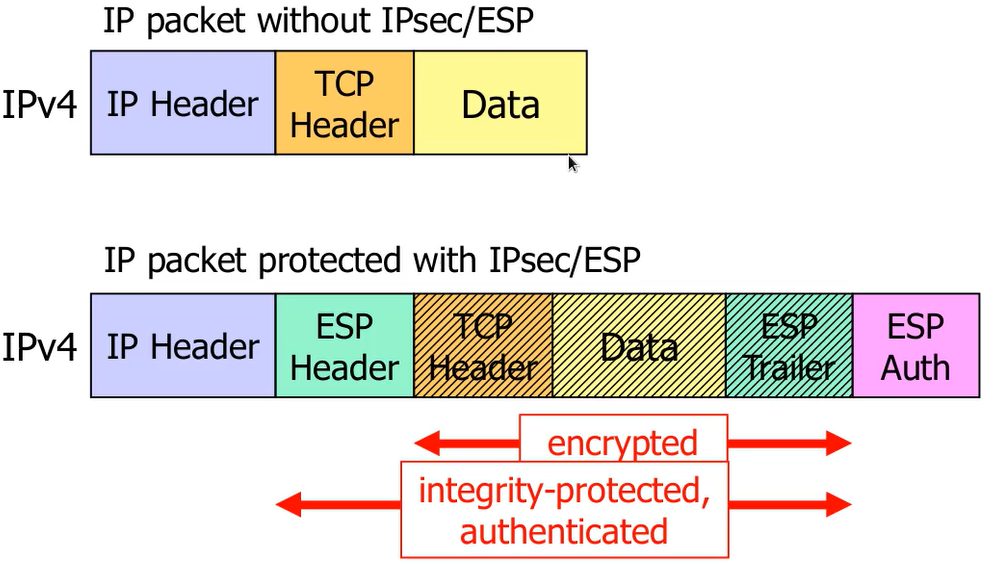
\includegraphics[width=150px]{img/IPSecTransportMode.png}
	\captionof{figure}{Abbildung einer IPSec mittels Transport Mode}
	\label{fig:Abbildung einer IPSec mittels Transport Mode}
\end{Figure}

\begin{Figure}
\centering
\includegraphics[width=150px]{img/IPSecESPMode.png}
	\captionof{figure}{Abbildung einer IPSec mittels ESP Mode}
	\label{fig:Abbildung einer IPSec mittels ESP Mode}
\end{Figure}

\textit{Sequenznummer:}
\begin{itemize}
	\item IPSec dürfen Pakete immer verloren gehen, reordered oder dupliziert werden
	\item Man akzeptiert alle Pakete, welche SeqNr man noch nicht hatte
	\item Man dropped diese SeqNr welche man bereits hat
	\item Das darübergeordnete Protokoll kümmert sich um die ungeordnete Pakete nicht IPSec 
\end{itemize}

\textit{Internet Key Exchange (IKE):}
\begin{itemize}
	\item Analog zum Handshake in TLS
	\item Variante 1: Public Key-Crypto mit X.509
	\item Variante 2: Preshared Secrets
\end{itemize}

	\subsection{TLS vs. IPSec}
\begin{itemize}
	\item Möchte man die Kommunikation zwischen zwei Applikationen sichern $\Rightarrow$ TLS
	\item Möchte man die Kommunikation zwischen zwei Hosts oder Anwendungen welche TLS nicht unterstützten $\Rightarrow$ IPSec
	\item IPSec zu konfigurieren ist keine triviale Aufgabe, da ist TLS einfacher!
\end{itemize}


\chapter{Vorlesung 9 - Virtual Private Networks (VPN)}

\section{Sie verstehen das Konzept von Virtual Private Network}
\begin{itemize}
	\item Geschütztes Netzwerk innerhalb eines öffentlichen Netzwerks 
	\item Aussenstehende von diesem Netzwerk können weder lesen noch modifizieren
	\item Sichere Verbindung zwischen Netzwerken
	\item VPN-Gateways sind die sicheren Endpunkte eines VPNs
	\item der sichere Kanal wird häufig \textit{Secure Channel} genannt
\end{itemize}

\section{Sie wissen und verstehen die zwei wichtigsten Protokolle um VPNs zu bauen (IPSec und OpenVPN) und können erklären, wie diese funktionieren sowie die Unterschiede aufzeigen}
\begin{itemize}
	\item IPSec und OpenVPN sind die beiden Standards
\end{itemize}


	\subsection{IPSec}
\begin{itemize}
	\item Schwierig zu konfigurieren
\end{itemize}

\textit{Tunnel Mode mit ESP}
\begin{itemize}
	\item Alles kommt in ein neue IP-Paket
	\item Neuer IP-Header
	\item kann die Struktur vor Dritte schützen
	\item Vorteil: Gibt es schon länger und gibt kommerzielle Produkte inkl. Support dafür
\end{itemize}

\begin{Figure}
\centering
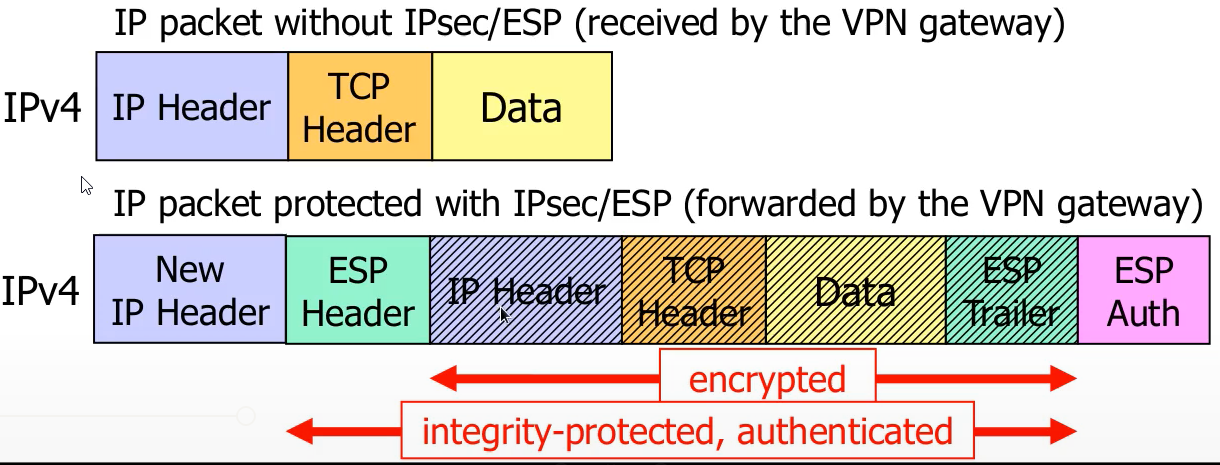
\includegraphics[width=150px]{img/vpnIpSecTunnelModeESP.png}
	\captionof{figure}{Abbildung über das Schema für VPN Tunnel Mode über ESP}
	\label{fig:Abbildung über das Schema für VPN Tunnel Mode über ESP}
\end{Figure}


	\subsection{OpenVPN}
\begin{itemize}
	\item einfacher zu konfigurieren
	\item Teil von TLS
	\item Opensource Projekt
	\item Baut auf dem Application Layer
	\item Läuft im User-Space, Nicht(!) im Kernel Space
	\item Endausbau identisch zu IPSec, jedoch anderen Aufbau
	\item Vorteil: weniger Features, einfachere Konfiguration, läuft im UserSpace
\end{itemize}

\begin{Figure}
\centering
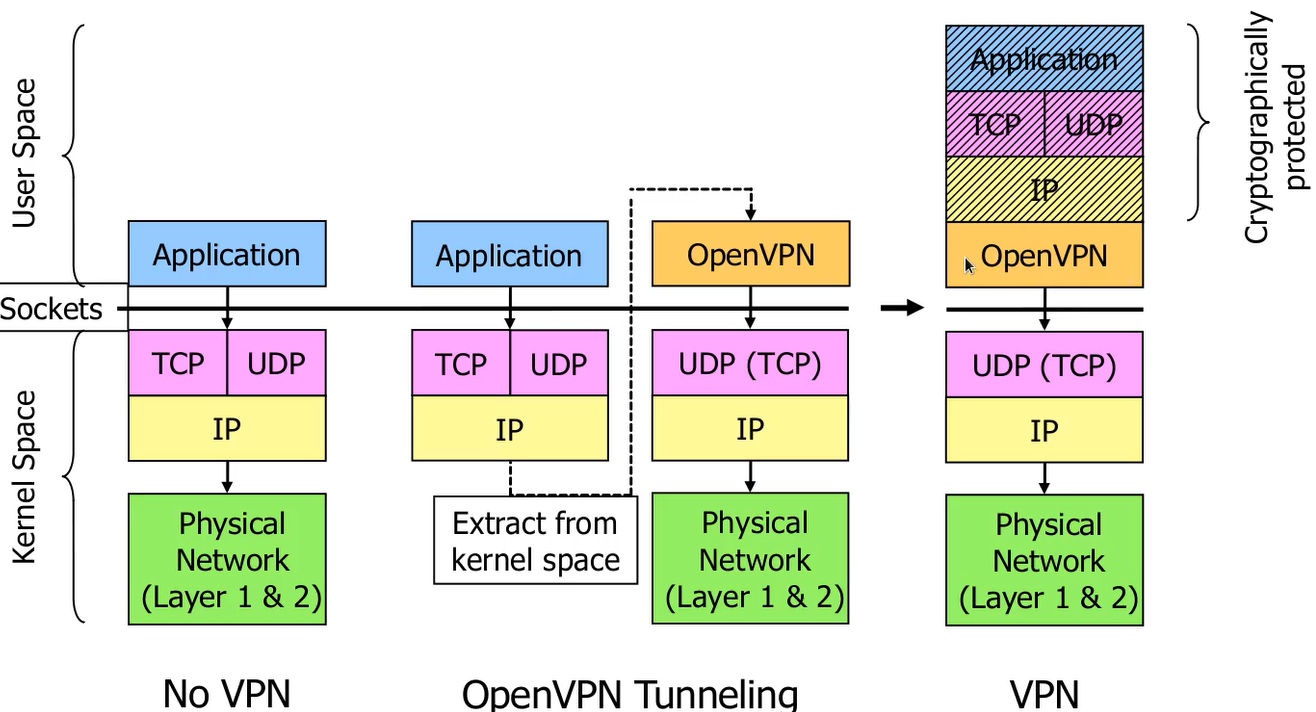
\includegraphics[width=150px]{img/vpnOpenVPNTunnelMode.png}
	\captionof{figure}{Abbildung über das Schema für VPN Tunnel Mode mittels OpenVPN}
	\label{fig:Abbildung über das Schema für VPN Tunnel Mode mittels OpenVPN}
\end{Figure}
$\Rightarrow$ Wird UDP verwendet, da es sonst TCP over TCP gäbe, das funktioniert in der Regel jedoch nicht $\rightarrow$ UDP funktioniert problemlos

\begin{Figure}
\centering
\includegraphics[width=150px]{img/vpnOpenVPN.png}
	\captionof{figure}{Abbildung über das Schema mittels OpenVPN}
	\label{fig:Abbildung über das Schema mittels OpenVPN}
\end{Figure}


\section{NICHT PrüfungsrelevantSie wissen vom Newcomer auf dem VPN Markt (WireGuard) und können den Unterschied zu IPSec und OpenVPN aufzeigen}
\begin{itemize}
	\item Neues VPN Produkt
	\item Arbeitet auf Layer3
	\item sehr vielversprechend
	\item Sehr wenige Dinge, welche konfiguriert werden kann (keine cipher und protocol agility $\rightarrow$ Es muss keine Verschlüsselungmethode ausgehandelt werden, beide Seiten sind mit Algorithmen bereits ausgerüstet)
	\item Verwendet moderne Crypto-primitives (ChaCha20, Curve25519)
	\item Handshake wird innerhalb eines RTT durchgeführt $\rightarrow$ schnellerer Verbindungsaufbau
	\item DoS-Attacken werden stark reduziert
\end{itemize}

\begin{Figure}
\centering
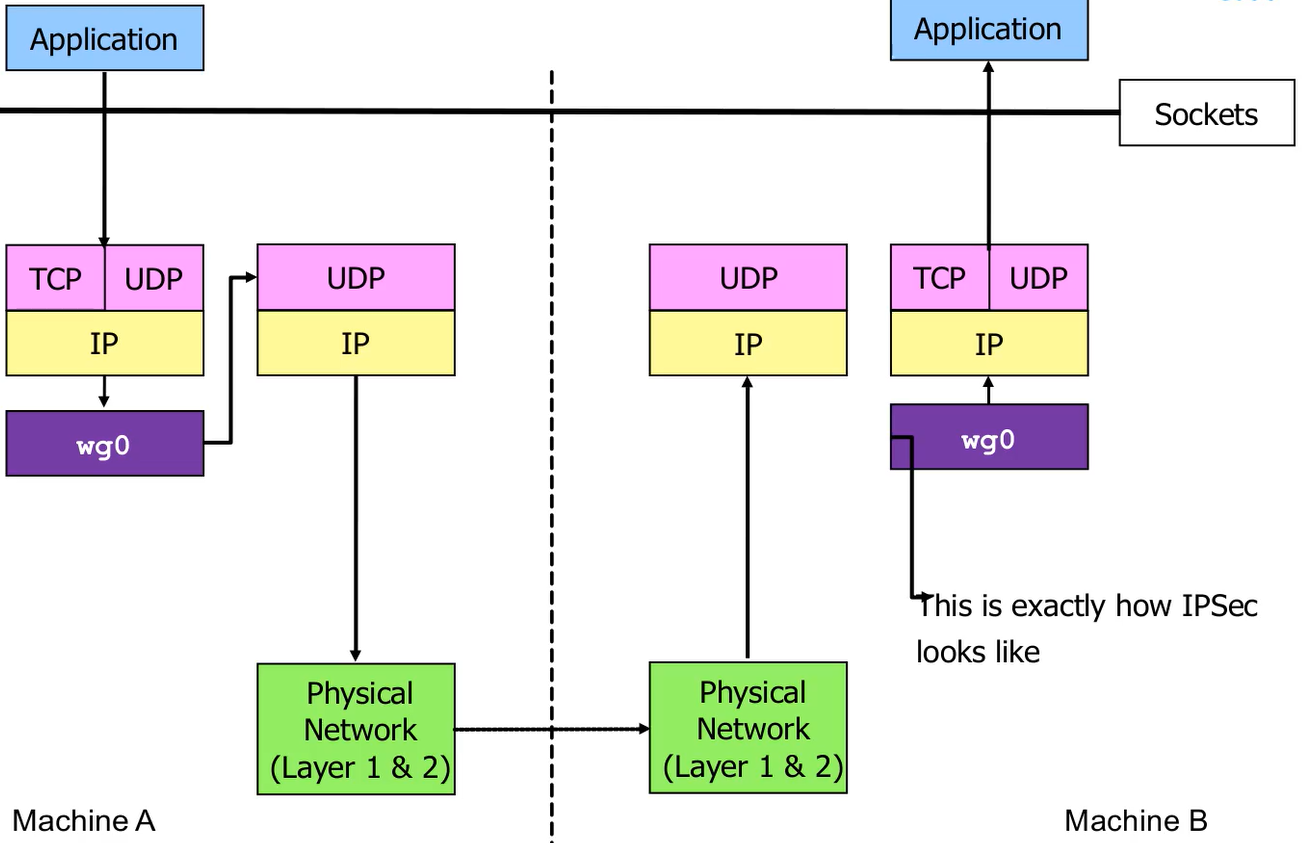
\includegraphics[width=150px]{img/WireGuardMessageFlow.png}
	\captionof{figure}{Abbildung über das Schema mittels WireGuard}
	\label{fig:Abbildung über das Schema mittels WireGuard}
\end{Figure}

\section{Sie kenne einige typische Anwendungsfälle von VPN und können diese erklären}
\begin{itemize}
	\item Sichere Verbindung von zwei oder mehreren remote Netzwerke
	\item selektiver Zugriff von Partner in einem Netzwerk
	\item Erlaubt den mobilen Zugriff
	\item Vorgaukeln, dass man sich in einem anderen Land verbindet
\end{itemize}

	\subsection{Firmennetzwerk mit einem Partnernetzwerk (bspw. Filiale)}
\begin{itemize}
	\item beiden Netzwerke sind mittels VPN verbunden
	\item Rechner wissen nicht, dass sie nur über ein VPN verbunden sind
\end{itemize}

\begin{Figure}
\centering
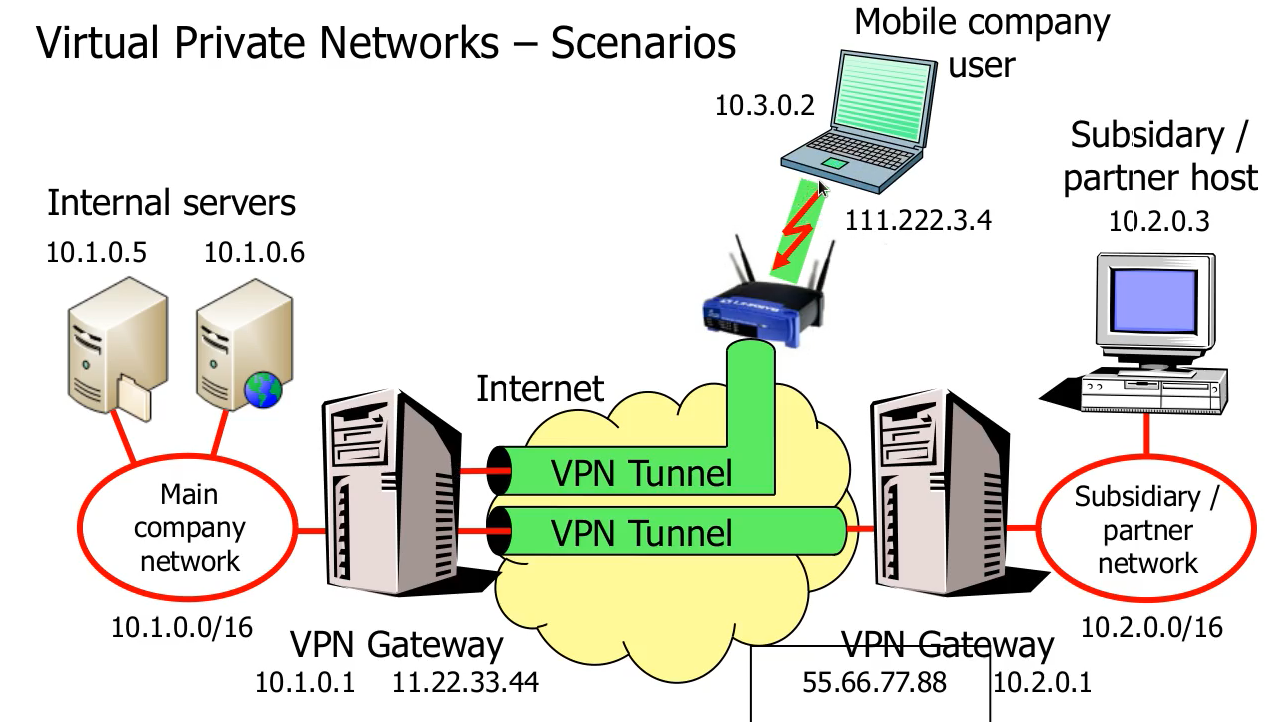
\includegraphics[width=150px]{img/VPNScenariosI.png}
	\captionof{figure}{Abbildung eines möglichen VPN-Szenarios(1)}
	\label{fig:Abbildung eines möglichen VPN-Szenarios(1)}
\end{Figure}

	\subsection{Mobile Company User Case}
Mobiler User braucht Zugang zum Netzwerk der Firma mittels dynamischer IP (bspw. zuhause, Hotel etc)\\
$\rightarrow$ Man weist dem mobilen User eine virtuelle IP addresse zu 

\begin{Figure}
\centering
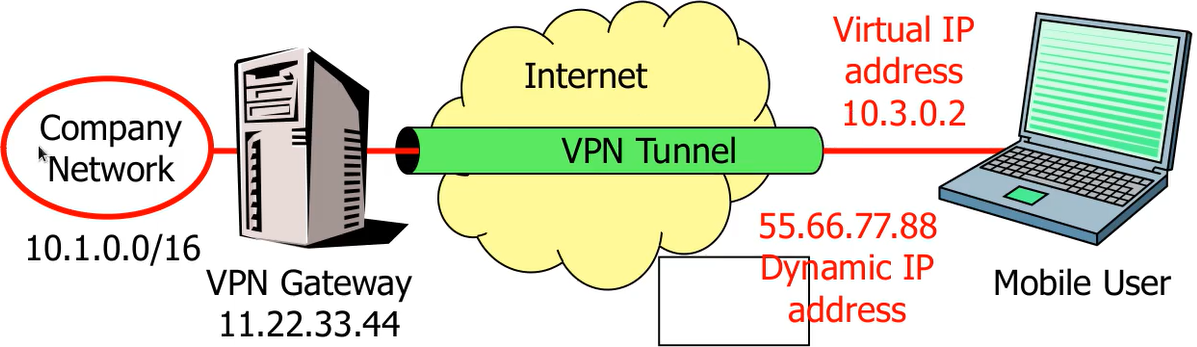
\includegraphics[width=150px]{img/VPNScenariosII.png}
	\captionof{figure}{Abbildung eines möglichen VPN-Szenarios(2)}
	\label{fig:Abbildung eines möglichen VPN-Szenarios(2)}
\end{Figure}


\chapter{Vorlesung 10 - User Authentication and Authentication Protocols}

\section{Sie kennen die Begrifflichkeiten Identifikation, Authentifizierung, Autorisierung und Accounting}
\textbf{Identifikation} Ich bin der User xyz, dafür brauche ich die \textbf{Authentifizierung} welche ich mittels Passwort (Credentials) bestätige. 
Danach kann ich im System nur diese Teile des Systems verwende, für welche ich auch zugelassen \textbf{Autorisierung}. Das ganze wird getracked mittels \textbf{Accounting}\\
$\Rightarrow$ das ganze wird als \textbf{User-Access} zusammengefasst

\begin{itemize}
	\item Authentication $\neq$ Identification
	\item Authentication $\neq$ Authorization
	\item Authentication $\neq$ Accounting
\end{itemize}

\begin{Figure}
\centering
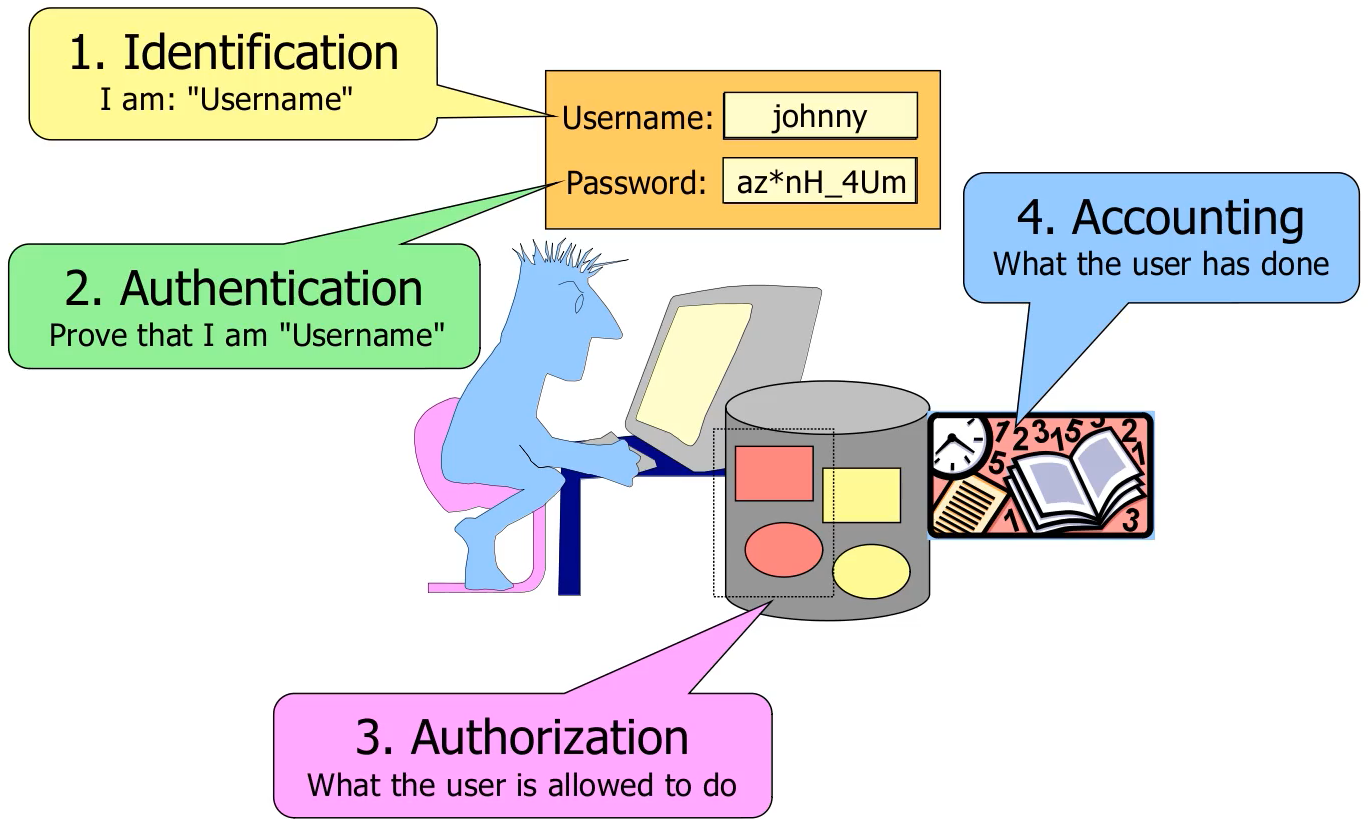
\includegraphics[width=150px]{img/Terminology.png}
	\captionof{figure}{Abbildung der Terminologien}
	\label{fig:Abbildung der Terminologien}
\end{Figure}

\section{Sie kennen den Unterschied zwischen den Authentication-facotrs und verstehen das heutige zwei-Weg-Authentifizierung-Schema}
Dies kann auf drei Methoden geschehen - User Authetnication basierend:
\begin{enumerate}
	\item auf dem wo man weiss (Passwort, Pin, Shared Secret) $\rightarrow$ etwas das nur der User weiss
	\item auf dem was man hat (Smartcard / Private Key, Token, mobile) $\rightarrow$ Überprüfung auf die Präsenz des echten Users
	\item auf dem was man ist (physiologische Pattern, Fingerabdruck, Voiceprints, Gesichtserkennung) $\rightarrow$ biologische Erkennung
\end{enumerate}

\textbf{Definition Zwei-Faktor Authentifzierung}: Man kombiniert zwei verschiedene der drei oben genannten Methoden um den User zu authentifzieren
	\subsection{Zweiweg Faktor Authentifzierung}
\begin{itemize}
	\item Heute sehr häufig im Einsatz
	\item häufig ist die One-Time Password (OTP) im Einsatz
	\item Der Zweite Faktor, soll nicht die gleichen Problematiken haben wie der erste Faktor (gegeben durch die vers. Methoden)
	\item OTP sind sehr einfach zu attackieren (E-Mail Phising) in der 1. Generation
	\item OTP 2. Generation durch challenge-response based approach: Durch eine Web-Sessions werden diese erst durch die eigentliche Session gechallenged und die response ist gewährleistet $\rightarrow$ MITM-Attacken sind weiterhin möglich
	\item OTP 3. Generation ist Kostengetrieben und nicht Sicherheitsgetrieben, durch mobile Apps auf dem Handy (keine Improvements im Vergleich zur 2. Generation) $\rightarrow$ Angriffe gegen das Handy
\end{itemize}

\section{Sie verstehen das Basis Prinzip von direkter und indirekter User Authentifizierung}
\textbf{direkte user authentication}
\begin{itemize}
	\item User sendet dem Host die Credentials
	\item Host hat alle Informationen um den User zu authentifizieren
	\item $\rightarrow$ Man muss dies für jede einzelne Anwendung machen kann sehr effizient werden
	\item $\rightarrow$ Sicherstellen, dass kein Passwort im Klartext übermittelt wird bei einem Remotezugriff
\end{itemize}

\begin{Figure}
\centering
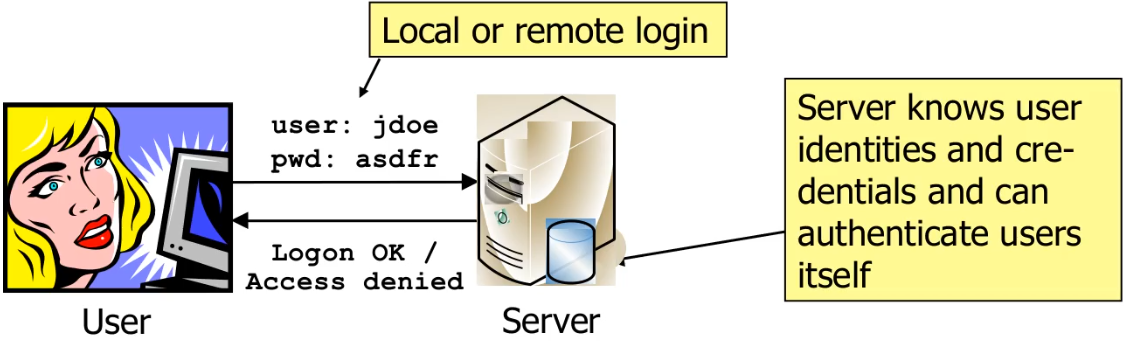
\includegraphics[width=150px]{img/directUserAuthentication.png}
	\captionof{figure}{Abbildung des Schemas bei der direkt Version}
	\label{fig:Abbildung der Terminologien}
\end{Figure}

\textbf{indirekte user authentication}
\begin{itemize}
	\item User sendet dem Host die Credentials
	\item Host kann den User nicht direkt authentifzieren
	\item Es kommt einen zusätzlichen \textit{authentication server} zum Einsatz $\rightarrow$ bspw. RADIUS, NTLM, Kerberos, Shibboleth
	\item $\rightarrow$ Eine zentrale Stelle $\Rightarrow$ Single-Sign-On möglich
	\item Nachteil: Single Point of Failure und beliebtes Ziel für Angriffe, muss speziell gesichert werden
\end{itemize}

\begin{Figure}
\centering
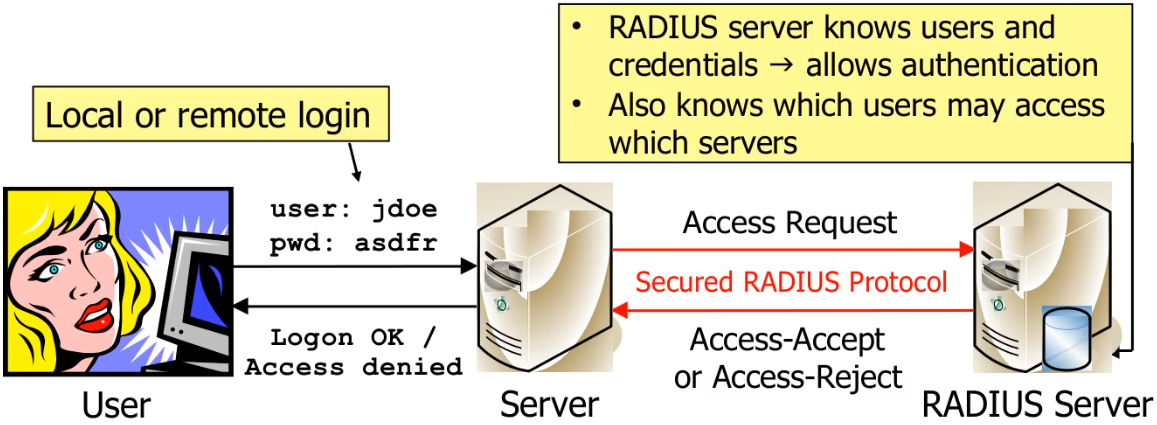
\includegraphics[width=150px]{img/indirectUserAuthentication.png}
	\captionof{figure}{Abbildung des Schemas bei der indirekt Version mit RADIUS}
	\label{fig:Abbildung der Terminologien}
\end{Figure}


\section{Sie verstehen die NTLM und Kerberos Protokolle, inklusive deren Sicherheitseigenschaften sowie Vor- und Nachteile}
Die Protokolle sind sehr nützlich für die Authentifzierung bei vielen Usern und dazu kommt noch das Key-Establishment.

	\subsection{Window NT LAN Manager (NTLM)}
\begin{itemize}
	\item Gibt einen Domain Controller (DC)
	\item DC kann Benutzer authentifzieren
	\item Windows Domain verwendet den DC
	\item DC ermöglicht Single Sign On (SSO)
\end{itemize}
\begin{Figure}
\centering
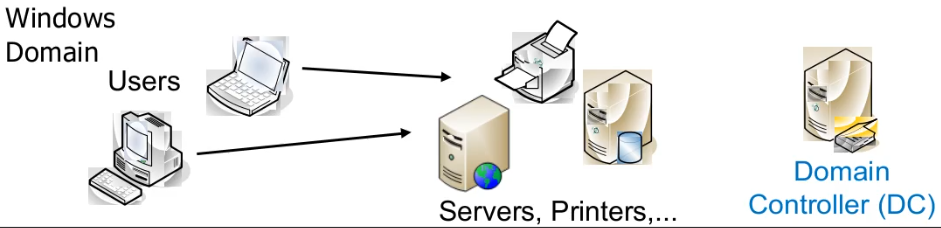
\includegraphics[width=150px]{img/DC.png}
	\captionof{figure}{Abbildung des Schemas für einen Domain Controller}
	\label{fig:Abbildung des Schemas für einen Domain Controller}
\end{Figure}

\begin{enumerate}
	\item Nach dem Aufstarten des PC muss man sich in der Domaine mittels username und password einloggen
	\item ein MD4-Hash des Passworts wird auf dem Computer berechnet (Key) und der Computer vergisst wieder dieses Passwort $\rightarrow$ DC kennt ebenfalls diesen Key (Shared Secret)
	\item Wenn auf den Server zugegriffen wird, fragt der Server den DC ob der User authentifziert ist für diesen Server und dies geschieht transparent (SSO)
\end{enumerate}

\begin{Figure}
\centering
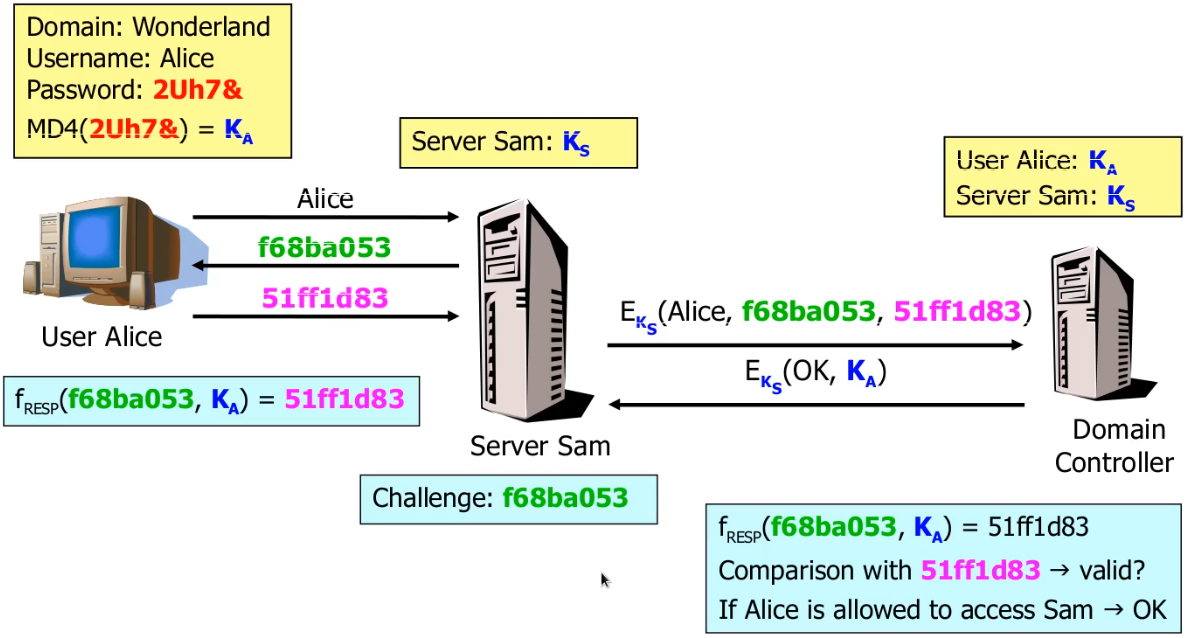
\includegraphics[width=150px]{img/NTLM.png}
	\captionof{figure}{Abbildung des Schemas für NTLM Protocol}
	\label{fig:Abbildung des Schemas für NTLM Protocol}
\end{Figure}
\textit{Was ist gut an diesem Protokoll?}
\begin{itemize}
	\item Komplexität ist tieferen
	\item Password werden nie im Klartext übermittelt $\rightarrow$ keine MITM-Attacken möglich
	\item Durch Zufalls Challenge-Response sind keine Replay-Attacken möglich
	\item Server lernt Schlüssel des Users kennen
\end{itemize}

\textit{Was ist schlecht an diesem Protokoll?}
\begin{itemize}
	\item Muss für jede Benutzung neu durchgeführt werden $\rightarrow$ hohe Belastung auf dem DC
	\item Keine wechselseitige-Authentification $\rightarrow$ keine Serverauthentifikation
	\item Server lernt Schlüssel des Users kennen $\rightarrow$ Langzeitgeheimnis wird bekannt
\end{itemize}
$\Rightarrow$ Wurde durch Kerberos abgelöst

	\subsection{Kerberos}
\begin{itemize}
	\item Hauptziel User Authentication in IP Netzwerk
	\item Verwendung von secret keys (no public key) cryptography
	\item letztes update 2005
\end{itemize}

\textit{Details:}
\begin{itemize}
	\item Jeder Teilnehmer wird \textit{principal} genannt
	\item Jeder principal teilen ein gemeinsames Geheimnis (the principal's master key) mit einem zentralisierten Server $\rightarrow$ Key Distributino Center (KDC)
	\item Alle Principal vertrauen dem KDC
	\item Die Kommunikation, Authentifikation und SessionKey-Verteilung geschieht über KDC
	\item Verwendet Ticket-Based Ansatz
	\item Kerberos ist der bevorzugte Dienst in Windows
\end{itemize}

\begin{Figure}
\centering
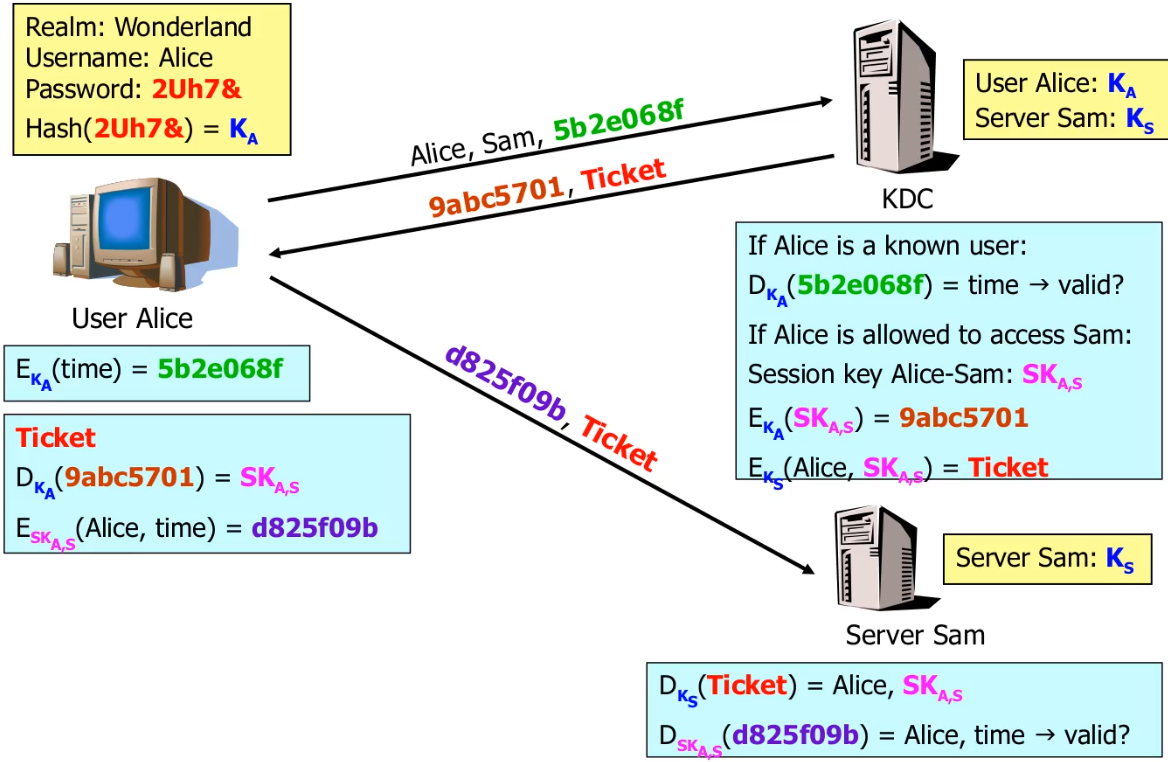
\includegraphics[width=150px]{img/Kerberos.png}
	\captionof{figure}{Abbildung des Schemas für ein sehr vereinfachtes Kerberos Protokoll}
	\label{fig:Abbildung des Schemas für ein sehr vereinfachtes Kerberos Protokoll}
\end{Figure}

Kerberos ist in zwei Schritte aufgeteilt:
\begin{enumerate}
	\item Authentication Service (AS) $\rightarrow$ User erhalten ein Ticket-Granting Ticket (TGT) welches bspw. 12h gültig ist
	\item Ticket-Granting Service (TGS) $\rightarrow$ erstellt Tickets für den Zugriff-Service
\end{enumerate}

\begin{Figure}
\centering
\includegraphics[width=150px]{img/KerberosV5AS.png}
	\captionof{figure}{Abbildung des Schemas für den AS Kerberos Protokoll Getting a Ticket}
	\label{fig:Abbildung des Schemas für den AS Kerberos Protokoll Getting a Ticket}
\end{Figure}

\begin{Figure}
\centering
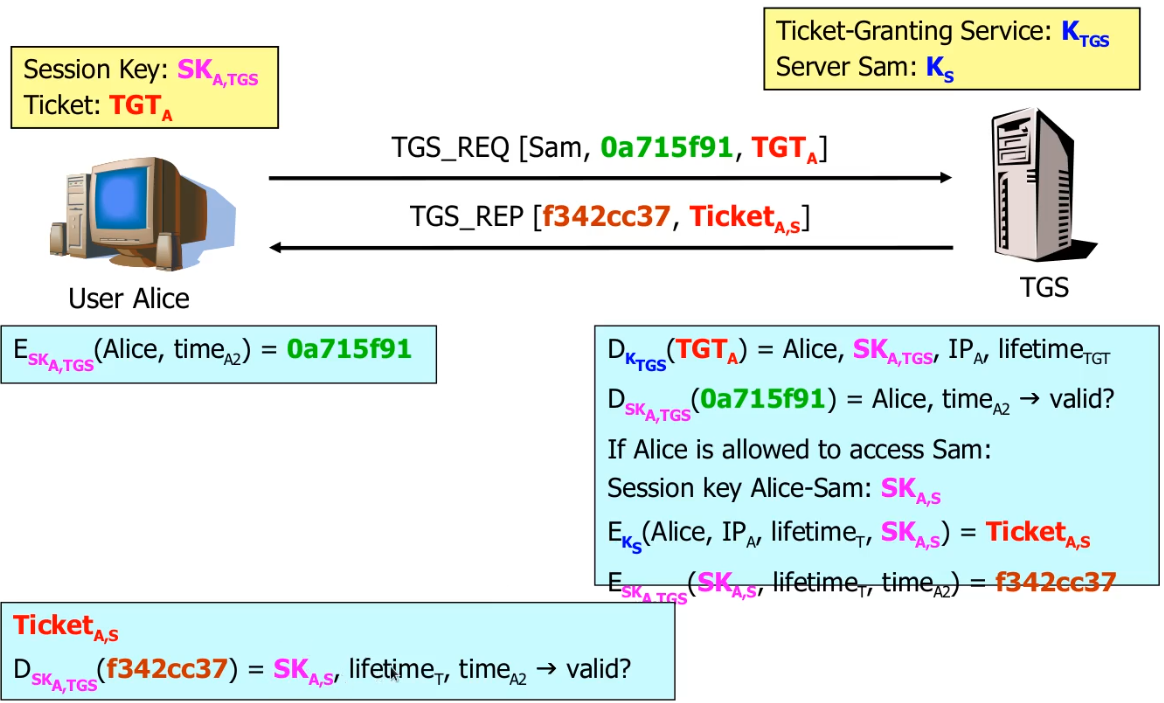
\includegraphics[width=150px]{img/KerberosV5TGT.png}
	\captionof{figure}{Abbildung des Schemas für den AS Kerberos Protokoll Requesting a ticket for accessing server sam}
	\label{fig:Abbildung des Schemas für den AS Kerberos Protokoll Requesting a ticket for accessing server sam}
\end{Figure}

\begin{Figure}
\centering
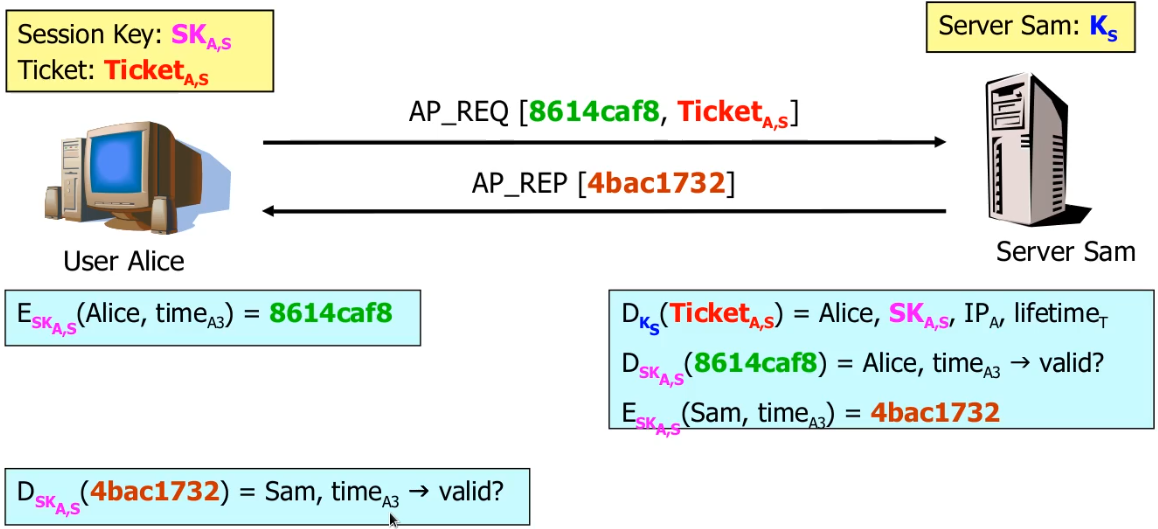
\includegraphics[width=150px]{img/KerberosV5Authentication.png}
	\captionof{figure}{Abbildung des Schemas für den AS Kerberos Protokoll accessing server sam}
	\label{fig:Abbildung des Schemas für den AS Kerberos Protokoll accessing server sam}
\end{Figure}

$\Rightarrow$ Ist sehr viel effizienter als NTLM
$\Rightarrow$ Es müssen alle das gleiche Verständnis und synchronisierte Zeit haben

		\subsubsection{Inter-Realm authentication}
Zwei verschiedene KDC verbinden sich mittels einem gemeinsamen geteilten Key
\begin{Figure}
\centering
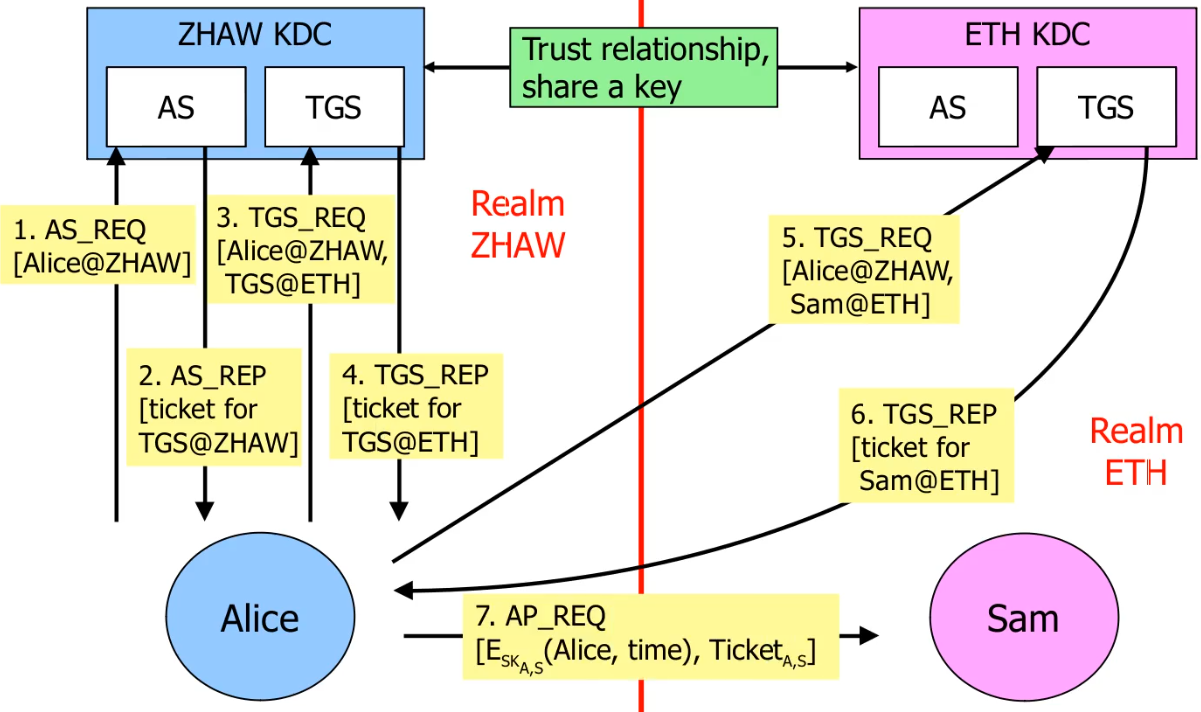
\includegraphics[width=150px]{img/InterRealmAuthentication.png}
	\captionof{figure}{Abbildung des Schemas für den federated Authentication mittels Keberos}
	\label{fig:Abbildung des Schemas für den federated Authentication mittels Keberos}
\end{Figure}

\section{Sie kennen die Bedeutung der federated authentication (and authorization) und verstehen wie diese in Shibboleth implementiert wird}
\begin{itemize}
	\item Shibboleth ist ein System für ein federated identity Management
	\item Wir haben Security Domains in verschiedenen Domains (bspw. ZHAW und ETH), welche kooperieren möchten
	\item Authentikation findet immer nur in der Homebase statt
	\item privacy preserving authentication ist möglich (Werte der genauen Eigenscahften müssen nicht weitergegeben werden bspw. ist über 18y alt)
\end{itemize}

\textit{Komponenten}
\begin{itemize}
	\item Organisationen (Firmen, Universitäten etc.)
	\item Users
	\item Service Provides (SP) (Service bspw. Drucker etc.)
	\item identity providers (IdP) Create tokens to access a SP
	\item Discovery Service: used to determine a user's home organization (IdP)
	\item das ganze ist Protokoll basierend (HTTPS und SAML (Security Assertion Markup Language))
\end{itemize}
\begin{Figure}
\centering
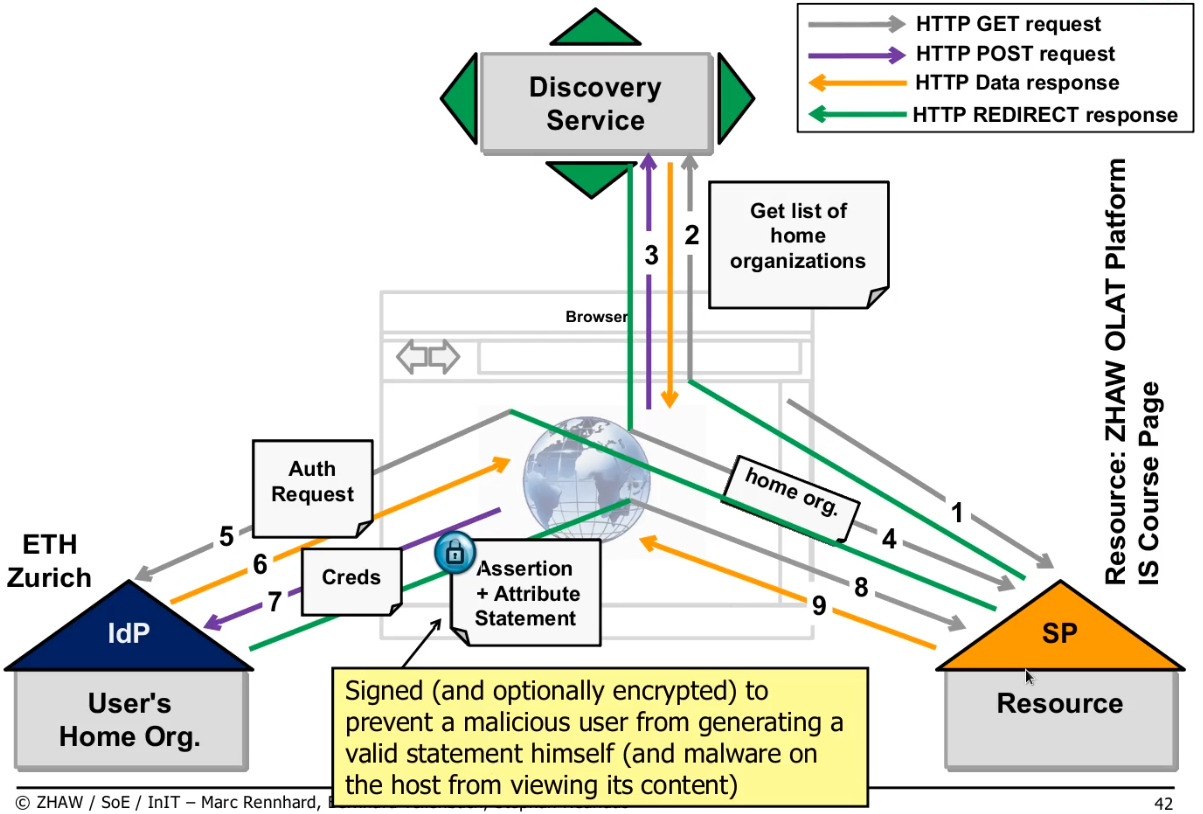
\includegraphics[width=150px]{img/Shibboleth.png}
	\captionof{figure}{Abbildung des Schemas für Shibboleth}
	\label{fig:Abbildung des Schemas für Shibboleth}
\end{Figure}


\chapter{Vorlesung 11 - Authorization}

\section{Sie können erklären was Authorization ist und können dazu die richtige Begriffe und das high-level Konzept erklären}
	\begin{itemize}
		\item Nach der erfolgreichen Authentifikation, kommt die Autorisierung
		\item Autorisierung ist in jedem Betriebssystem und Anwendung vorhanden
	\end{itemize}

	\subsection{Reference Monitor}
Sind dazu da, die Autorisierung entsprechend durchzusetzen $\rightarrow$ What \textbf{subjects} can perform what \textbf{operations} on what \textbf{objects}\\
\textbf{Terminologie:}
\begin{itemize}
	\item Subject oder Principal $\rightarrow$ real-world enitity: \textbf{User oder Computer} beziehungsweise computational enitity reagiert im Namen der authenifizierten real-world enitity bspw. \textbf{Prozess oder Thread}
	\item Object $\rightarrow$ \textbf{sichtbare Ressourcen} (Files, Printers, Sockets) oder \textbf{weniger sichtbare Ressourcen} (Systemprozesse oder Threads) oder grundlegende Systemaufgaben (Wechsel Systemzeit, Computer herunterfahren)
\end{itemize}

\begin{itemize}
	\item Vor jeder sensiblen Aktion, muss der Reference Monitor geöffnet werden
	\item Schaut in der security policy nach
	\item je nach Entscheid kann die Operation (schreiben, lesen etc) durchgeführt werden
	\item $\rightarrow$ trusted computer base
\end{itemize}



\section{Sie kennen die drei Access-Control-Models und verstehen wie diese eingesetzt werden können}

	\subsection{Discretionary Access-Control (DAC)}
\begin{itemize}
	\item Die Kontrolle des Object ist Sache des Owners
	\item Der Owner bestimmt wer was machen darf
	\item Owner erstellt Object für den User
	\item die meisten OS sind nach diesem Prinzip
	\item root (Linux), Administrator (Windows) darf DAC umgehen
	\item kann mittels ACL (Access Control List) implementiert werden
	\item ACL ist mitt dem Objekt verknüpft
	\item der reference Monitor nimmt folgendes entgegen \texit{check(subj, obj, action, ACL(obj))} $\Rightarrow$ Kann sehr komplex werden durch Vererbung
	\item Capabilities ist ein anderer Ansatz um DAC zu implementieren $\rightarrow$ Gibt wenige welche rein Capability-based sind (bspw. KERBEROS)
	\item Ein Capability ist ein Token für welches das Subject der Owner ist und die Berechtigungen verteilen kann
	\item der Reference Monitor prüft ob das Token echt ist und überprüft ob die Aktion durchgeführt werden darf
\end{itemize}
\begin{Figure}
\centering
\includegraphics[width=150px]{img/DAC.png}
	\captionof{figure}{Abbildung DAC}
	\label{fig:Abbildung DAC}
\end{Figure}

\textbf{ACL Windows vs. Linux}
\begin{Figure}
\centering
\includegraphics[width=150px]{img/ACLWvL.png}
	\captionof{figure}{Abbildung ACL in Windows vs. Linux}
	\label{fig:Abbildung ACL in Windows vs. Linux}
\end{Figure}

\textbf{ACL vs. Capabilities}
\begin{Figure}
\centering
\includegraphics[width=150px]{img/ACLvsCapI.png}
	\captionof{figure}{Abbildung ACL vs. Capabilities Part 1}
	\label{fig:Abbildung ACL vs. Capabilities Part 1}
\end{Figure}
\begin{Figure}
\centering
\includegraphics[width=150px]{img/ACLvsCapII.png}
	\captionof{figure}{Abbildung ACL vs. Capabilities Part 2}
	\label{fig:Abbildung ACL vs. Capabilities Part 2}
\end{Figure}

\textbf{Limitation von ACL: The Confused Deputy Problem}\\
$\rightarrow$ Trifft häufig dann auf, wenn die Person welche es implementiert nicht ganz verstanden hat wie ACL funktioniert
\begin{itemize}
	\item Dies passiert, wenn nur der Name der Ressource weitergegeben wird aber nicht die Ressource selbst
	\item Service muss programmatisch prüfen wer hat den Antrag gestellt und was darf diese Person ausführen
	\item Grundsätzlich kann das OS da nicht mehr durchblicken, aus diesem Grund müsste es im Compilation Service getätigt werden $\Rightarrow$ schöner wäre es, wenn dies jedoch delegiert werden kann, dazu kann man Capabilities verwenden
	\item Capability auch für Zieldatei mitgeben
\end{itemize}

\begin{Figure}
\centering
\includegraphics[width=150px]{img/confusedDeputyProblem.png}
	\captionof{figure}{Abbildung des confused Deputy Problems}
	\label{fig:Abbildung des confused Deputy Problems}
\end{Figure}

\begin{Figure}
\centering
\includegraphics[width=150px]{img/solveConfusedDeputyProblem.png}
	\captionof{figure}{Abbildung der Lösung confused Deputy Problems}
	\label{fig:Abbildung der Lösung confused Deputy Problems}
\end{Figure}

$\Rightarrow$ Man kann ACL und Capability kombinieren


	\subsection{Mandatory Access-Control (MAC)}
\begin{itemize}
	\item Zugriff entscheidet durch eine Systemweite Policy
	\item Owner kann dies nicht beeinflussen
	\item Kontrolle kann praktisch nicht umgehen
	\item bspw. Militär
	\item wird nur in kritischen Teilen verwendet
\end{itemize}

		\subsubsection{Bell-LaPadula Model}
\begin{itemize}
	\item Fokus liegt auf Vertraulichkeit
	\item Subjects welche nicht vertrauenswürdig sind, haben keinen Zugriff auf Subject
	\item vertrauenswürdige Subjects können Informationen nicht weitergegeben werden
	\item Multi-Level Security Jedes Subjekt und jedes Objekt hat ein Security-Level
	\item Simple Security property bzw. no read up $\rightarrow$ Das Objekt darf nicht eine Ebene höher lesen
	\item No write down $\rightarrow$ Subject darf nur schreiben wenn das Object auf der gleichen oder höhere Ebene liegt
\end{itemize}

		\subsubsection{Biba Model}
\begin{itemize}
	\item Fokus liegt auf Integrität
	\item No write Up $\rightarrow$ Kein Subjekt darf ein tieferes Objekt schreiben
	\item no read down $\rightarrow$ Kein Subjekt darf ein höheres Objekt lesen
\end{itemize}

	\subsection{Role-based Access Control (RBAC)}
\begin{itemize}
	\item DAC und MAC sind sehr technisch (subject, object) $\rightarrow$ Funktioniert weniger für echte user
	\item Man möchte Zugriff auf Basis von der Jobrolle freigeben / blockieren
	\item Core RBAC (required) $\Rightarrow$ Minimumsammlung an Elemente die man braucht um RBAC durchzuführen
	\item Hierarchical (optional)
	\item Constraint (optional)
	\item Rolle definiert eine Menge an Transaktionen, welche Member dürfen
	\item Transaction ist eine Transformationprozedur (bspw. Datenbank update) plus ein dazugehöriges Objekt
	\item RBAC unterstützt das \textit{principle of least privilege (or authority)}
	\item RBAC unterstützt \texit{Separation of duties} $\Rightarrow$ Vier-Augen-Prinzip - um eine bestimmte Action zu autorisieren braucht man zwei unterschiedliche Rollen
	\item RBAC unterstütz \textit{Data Abstraction}
	\item RBAC wird nicht vom OS unterstützt (Anwendungen brauchen eigene Reference Monitor)
	\item Vererbung bei RBAC ist limitiert auf Single dimension roles
	\item RBAC ist erweiterbar mit ABAC (Attribute-Based Access Control) bspw. Geschlecht, Zivilstand, Aktuelle Zeit, Location $\rightarrow$ bspw. sehr einfach für \textit{Nur Kunden über 18 Jahre}
\end{itemize}

	\subsection{DAC vs. MAC vs. RBAC}
\begin{Figure}
\centering
\includegraphics[width=150px]{img/AccessControlModels.png}
	\captionof{figure}{Abbildung einer Übersicht der verschiedenen Modellen}
	\label{fig:Abbildung einer Übersicht der verschiedenen Modellen}
\end{Figure}

\section{Sie verstehen welche Bausteine man braucht um die drei Modelle zu erstellen}
\begin{itemize}
	\item Conceptual Framework
	\item security policy
	\item security mechanism
\end{itemize}

	\subsection{Conceptual Framework}
\begin{itemize}
	\item Discretionary Access Control
	\item Mandatory Access Control
	\item Role-Based Control (RBAC)
\end{itemize}

	\subsection{Security Police}
\begin{itemize}
	\item Definiert wer was wann tun darf
	\item Schwierigkeit $\rightarrow$ das korrekte Level von Zugriff
	\item Muss flexibel und mit Respekt zur Konfiguration sein
	\item Zugriff muss auf Basis von verschiedenen Kriterien erfolgen (bspw. Job-Rolle, Gruppe, aktueller Standort, Operation [read, write etc])
\end{itemize}
Theoretisch definiert das Management die Security policy und der Security Administrator implementiert und erfüllt diese Policy

	\subsection{Security Mechanism}
\begin{itemize}
	\item ist die eigentliche Methode welche die security policy implementiert
	\item im Sinne einer Matrix zwischen Subject und Object
\end{itemize}
\begin{Figure}
\centering
\includegraphics[width=150px]{img/SecurityMechansimMatrix.png}
	\captionof{figure}{Abbildung einer Beispielmatrix des Security Mechanismus}
	\label{fig:Abbildung einer Beispielmatrix des Security Mechanismus}
\end{Figure}
$\Rightarrow$ Ist für die praktische Anwendung nicht einsetzbar, sondern nur für konzeptionelle Überlegungen\\
\textbf{Access Control List (ACL)} An einem Object steht, welches Subject welche Operationen gemacht werden darf \\
\textbf{Capabilities} 

\section{Sie können die zwei Ansätze für Authorization in multi-tier Anwendungen hervorheben}

\begin{itemize}
	\item multi-tier ist typischerweise wie folgt: Presentation, Application processing (business logic), Data Management
	\item Häufig three-tier Architektur: Presentation tier, Logic tier, Data tier
	\item bei multitier Anwendungen gibt es keine offensichtliche Verbindung zwischen User (Tier 1) und Anwendung (Tier 2 - n)
	\item Variante 1 - The Impersonation / delegation model: Benutzeridentität auf Tier 1 überlebt für die nächsten Tiers
	\item Variante 2 - The trusted application model: Die Benutzeridentität überlebt nicht zum middle tier, hingegen the middle tier accesses the next tier using a generic (and relatively high-privileged) service Account $\Rightarrow$ dominierende Variante in der Praxis (bspw. WebApp)	
\end{itemize}

	\subsection{The Impersonation / Delegation Model}
\begin{itemize}
	\item Subject überlebt auch nach dem middle tier
	\item Subject access token kann weitergeleitet werden
\end{itemize}
\begin{Figure}
\centering
\includegraphics[width=150px]{img/impersonation.png}
	\captionof{figure}{Abbildung Schema Impersonation Model}
	\label{fig:Abbildung Schema Impersonation Model}
\end{Figure}

	\subsection{The Trusted Application Model}
\begin{itemize}
	\item Zugriff passiert mit standardisiertem Account (service Account)
	\item Request wird akzeptiert / abgelehnt basierend auf einem Set von policies
	\item policy check kann hardcodiert werden oder via API
\end{itemize}
\begin{Figure}
\centering
\includegraphics[width=150px]{img/TrustedApplicationModel.png}
	\captionof{figure}{Abbildung Schema Trusted Application Model}
	\label{fig:Abbildung Schema Trusted Application Model}
\end{Figure}

\section{Sie können für die verschiednen Models und Konzepte die Vor- und Nachteile nennen}
\begin{Figure}
\centering
\includegraphics[width=150px]{img/ImpersVsTrusted.png}
	\captionof{figure}{Abbildung Vergleich zwischen Impersonation und Trusted Application Model}
	\label{fig:Abbildung Vergleich zwischen Impersonation und Trusted Application Model}
\end{Figure}


\end{document}